% vim: tw=0:wrap:linebreak
\documentclass[DM,toc,lsstdraft]{lsstdoc}

\usepackage{datetime}
\usepackage{microtype}

\newcommand{\microarcsec}{$\mu$as\xspace}
\interfootnotelinepenalty=10000

\setcounter{secnumdepth}{3}

\title{Data Management Science Pipelines Design}
\author{
    J.D.~Swinbank,
    T.~Axelrod,  A.C.~Becker, J.~Becla, E.~Bellm,
    J.F.~Bosch,  H.~Chiang, D.R.~Ciardi,  A.J.~Connolly,  G.P.~Dubois-Felsmann,
    F.~Economou, M.~Fisher-Levine, M.~Graham, \v{Z}. Ivezi\'c,  M.~Juri\'c,
    T.~Jenness,  R.L.~Jones, J.~Kantor, S.~Krughoff, K-T.~Lim, R.H.~Lupton,
    F.~Mueller,  D.~Petravick, P.A.~Price,  D.J.~Reiss, D.~Shaw, C.~Slater,
    M.~Wood-Vasey, X.~Wu, P.~Yoachim,
     \emph{for the LSST Data Management}
}

\setDocRef{LDM-151}
\setDocCurator{J.D.~Swinbank}
\date{\today}

\setDocAbstract{%
The LSST Science Requirements Document (the LSST \SRD) specifies a set of data product guidelines, designed to support science goals envisioned to be enabled by the LSST observing program.
Following these guidlines, the details of these data products have been described in the LSST Data Products Definition Document (\DPDD), and captured in a formal flow-down from the \SRD via the LSST System Requirements (\LSR), Observatory System Specifications (\OSS), to the Data Management System Requirements (\DMSR).
The LSST Data Management subsystem's responsibilities include the design, implementation, deployment and execution of software pipelines necessary to generate these data products. This document describes the design of the scientific aspects of those pipelines.
}

%
%   Revision history
%
% OLDEST FIRST: VERSION, DATE, DESCRIPTION, OWNER NAME
\setDocChangeRecord{%
\addtohist{1}{2009-03-26}{Initial version as Document-7396}{Tim Axelrod et al.}
\addtohist{1.2}{2009-03-27}{Minor edits}{Tim Axelrod}
\addtohist{1.3}{2009-04-17}{General edits and updates}{Tim Axelrod}
\addtohist{1.4}{2009-05-08}{Explicit reference to multifit added to Section 6.1}{Tim Axelrod}
\addtohist{1.5}{2010-02-11}{General edits and updates; generated from SysML model}{Jeff Kantor}
\addtohist{2}{2011-08-04}{Elevated to LDM handle; general updates and edits}{Tim Axelrod}
\addtohist{3}{2013-10-07}{Updates for consistency with FDR baseline}{Mario Juric}
\addtohist{}{2017-05-08}{Major reorganization for DM replan}{Mario Juric}
\addtohist{4.0}{2017-05-19}{Approved in \href{https://jira.lsstcorp.org/browse/RFC-338}{RFC-338} and released.}{Mario Juric (approval), Tim Jenness (release)}
\addtohist{4.1}{2017-07-19}{Remove development commentary. This content was included erroneously and was not part of the approved baseline.}{Tim Jenness}
}


\begin{document}

\maketitle

\input{sections/preface}

\section{Introduction}

\subsection{LSST Data Management System}

To carry out this mission the Data Management System (DMS) performs the following major functions:

\begin{itemize}
\item Processes the incoming stream of images generated by the camera
  system during observing to produce transient alerts and to archive
  the raw images.

\item Roughly once per year, creates and archives a Data Release (``DR''),
  which is a static self-consistent collection of data products
  generated from all survey data taken from the date of survey
  initiation to the cutoff date for the Data Release. The data
  products (described in detail in the \DPDD), include measurements of 
  the properties (shapes, positions, fluxes, motions, etc.) of all detected
  objects, including those below the single visit sensitivity limit,
  astrometric and photometric calibration of the full survey object
  catalog, and limited classification of objects based on both their
  static properties and time-dependent behavior.  Deep coadded images
  of the full survey area are produced as well.

\item Periodically creates new calibration data products, such as bias
  frames and flat fields, that will be used by the other processing
  functions, as necessary to enable the creation of the data products above.

\item Makes all LSST data available through interfaces that utilize,
  to the maximum possible extent, community-based standards such as those
  being developed by the Virtual Observatory (``VO''), and facilitates user
  data analysis and the production of user-defined data products at Data
  Access Centers (``DAC'') and at external sites.
\end{itemize}

The overall architecture of the DMS is discussed in more detail in the Data Management System Design (\DMSD) document. The overall architecture of the DMS is shown in Figure~\ref{fig:DMS}.
\\

This document discusses the role of the Applications layer in the first three functions listed above (the functions involving \emph{science pipelines}).  The fourth is discussed separately in the SUI Conceptual Design Document (\SUI).

\begin{figure}
\centering
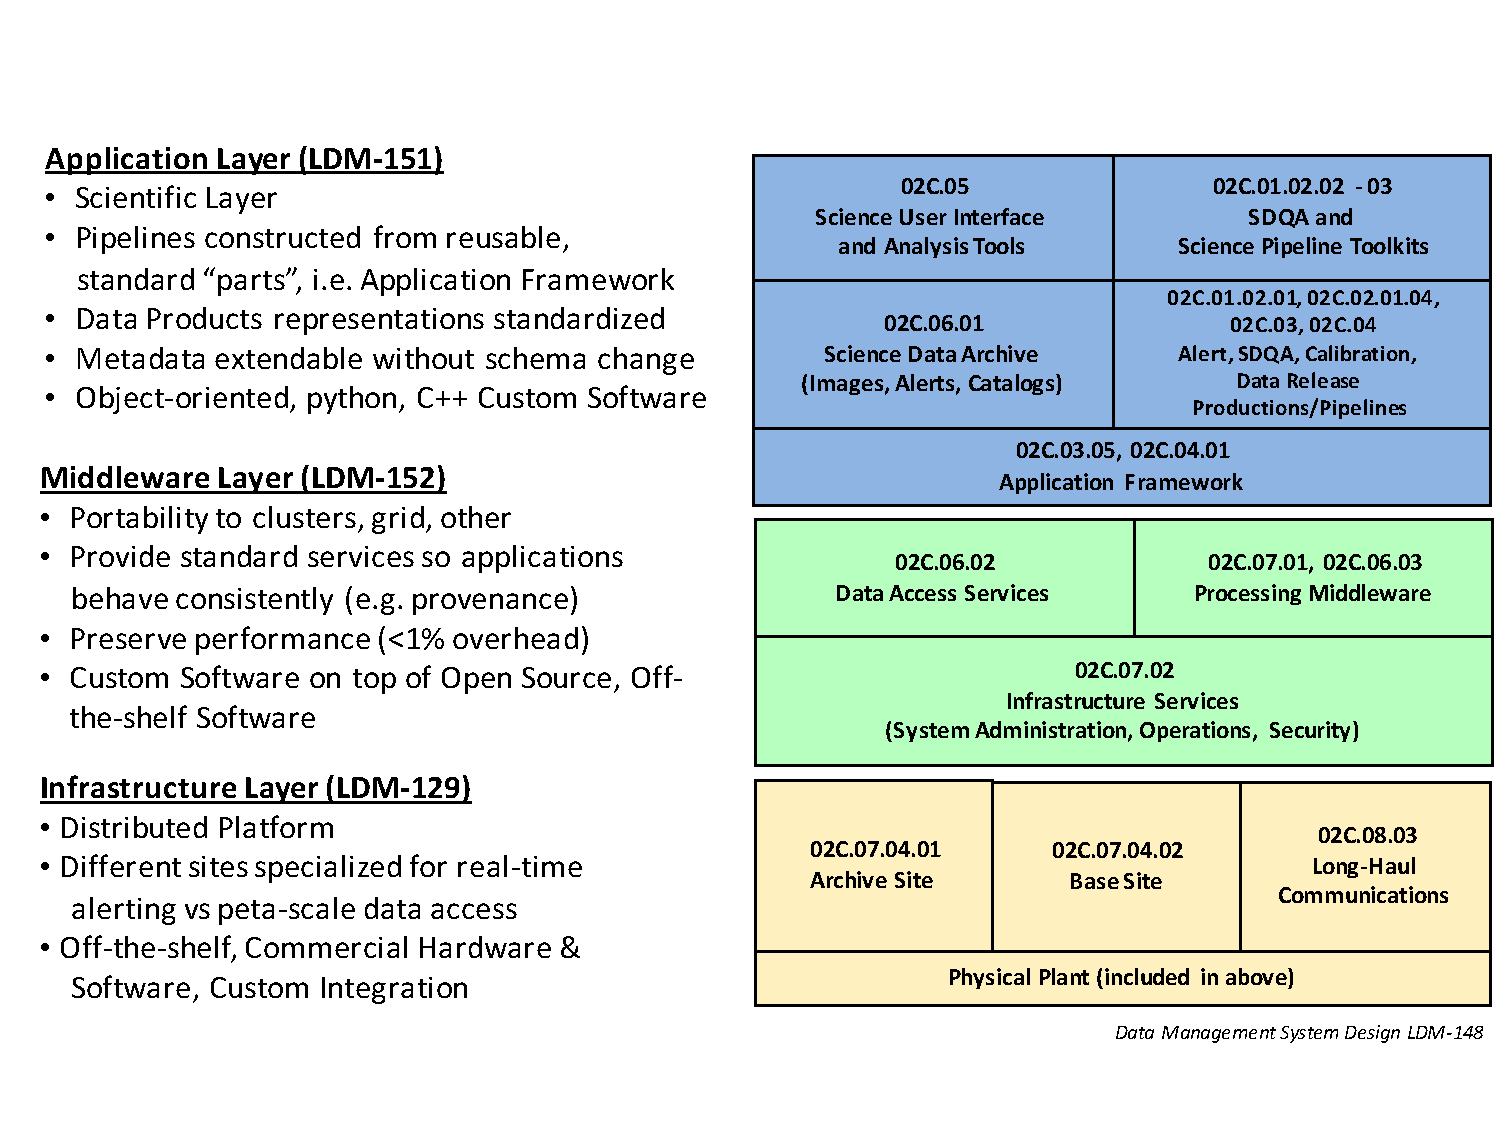
\includegraphics[angle=90,scale=0.70]{figures/DMS-Architecture.pdf}
\caption{Architecture of the Data Management System\label{fig:DMS}}
\end{figure}

\begin{figure}
%\includegraphics[angle=90,scale=0.70]{ApplicationLayerProductionsandPipelines.eps}
\centering
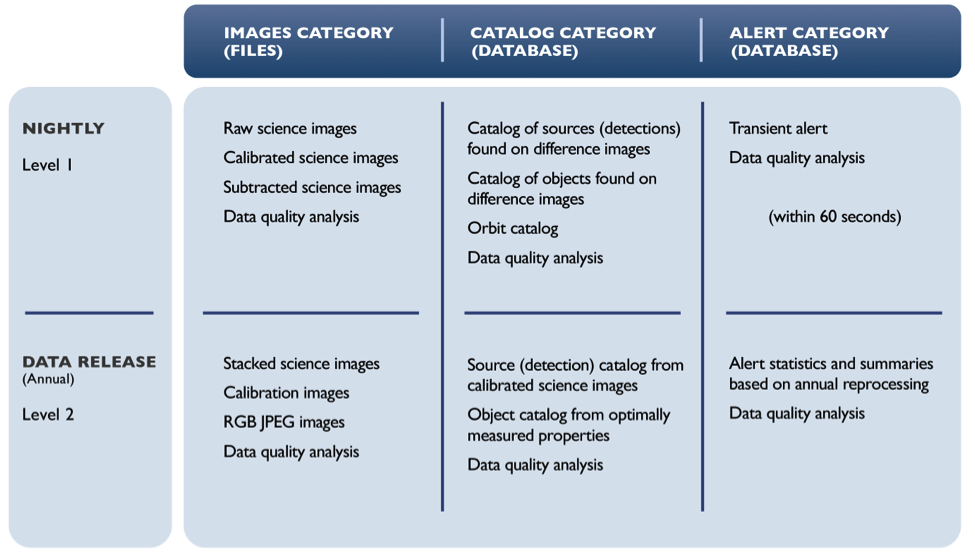
\includegraphics[angle=90]{figures/DataProductDelivarables.png}
\caption{Organization of LSST Data Products\label{fig:DP}}
\end{figure}

\subsection{Data Products}

The LSST data products are organized into three groups, based on their intended use and/or origin. The full description is provided in the Data Products Definition Document (\DPDD); we summarize the key properties here to provide the necessary context for the discussion to follow. 

\begin{itemize}
\item {\bf Level 1} products are intended to support timely detection and follow-up
  of time-domain events (variable and transient sources). They are generated by
  near-real-time processing the stream of data from the camera system during 
  normal observing.  Level 1 products are therefore continuously generated and / or
  updated every observing night. This process is of necessity highly
  automated, and must proceed with absolutely minimal human
  interaction.  In addition to science data products, a number of related
  Level 1 ``SDQA''\footnote{Science Data Quality Analysis} data products are generated
  to assess quality and to provide feedback to the Observatory Control System (OCS).

\item {\bf Level 2} products are generated as part of a Data Release, generally
  performed 
  yearly, with an additional data release for the first 6 months of survey data. 
  Level 2 includes data products for which extensive
  computation is required, often because they combine information from
  many exposures.  Although the steps that generate Level 2 products
  will be automated, significant human interaction may be required at
  key points to ensure the quality of the data.

\item {\bf Level 3} products are generated on any computing resources
  anywhere and then stored in an LSST Data Access Center. Often, but not
  necessarily, they will be generated by users of LSST using LSST software
  and/or hardware. LSST DM is required to facilitate the creation of
  Level 3 data products by providing suitable APIs, software components, and
  computing infrastructure, but will not by itself create any Level 3
  data products. Once created, Level 3 data products may be associated with
  Level 1 and Level 2 data products through database federation.
  Where appropriate, the LSST Project, with the agreement of the Level 3
  creators, may incorporate user-contributed Level 3 data product pipelines
  into the DMS production flow, thereby promoting them to Level 1 or 2.

\end{itemize}
%
The organization of LSST Data Products is shown in Figure~\ref{fig:DP}.

Level 1 and Level 2 data products that have passed quality control
tests will be accessible to the public without restriction.
Additionally, the source code used to generate them will be made
available, and LSST will provide support for builds on selected
platforms.

\subsection{Science Pipelines Overview}

We recognize four major groups of science pipelines residing in the Applications layer:
\begin{itemize}
    \item {\bf Level 1 Pipelines}, grouped under the {\bf Alert Production} element of the WBS, are designed to generate Level 1 data products. These include:
    \begin{itemize}
    \item {\bf \emph{Single Frame Processing (``SFM'') Pipeline}} (\wbsSFM), to reduce acquired visits and detect and characterize astrophysical sources present in these visits.
    \item {\bf \emph{Image Differencing Pipeline}} (\wbsDiffim), to create difference images, and detect and characterize sources in them.
    \item {\bf \emph{Association Pipeline}} (\wbsAssocP), to associate sources detected in the difference images with known objects.
    \item {\bf \emph{Alert Generation Pipeline}} (\wbsAP), to generate and transmit alerts to time-domain events (e.g., transients) to the astronomical community, and
    \item {\bf \emph{Moving Object Pipeline}} (\wbsMOPS), to identify, link and compute orbits for Solar System objects detected in difference images.
    \end{itemize}
Level 1 pipelines run as the data are being acquired. They primarily focus on image differencing, and the reduction of information extracted from difference images. The algorithms they employ are designed and chosen to complete processing on minute (alert production) to day (\textbf{\emph{DayMOPS}}) time scales. They are also rerun as a part of Data Release Production (DRP), potentially in somewhat different configurations to achieve greater precision at the expense of increased runtime.
    
    \item {\bf Level 2 Pipelines} run annually or semi-annualy (for the first year of data), and are designed to generate deep co-adds and catalogs stemming from analysis of direct image data.  These include:
    \begin{itemize}
        \item {\bf \emph{PSF Estimation Pipeline}} (\wbsPSF), to estimate the PSF properties and variation across the focal plane for each visit, to the degree of precision required by the \SRD. Note that the work of this pipeline goes beyond the typical single-CCD PSF estimation present in the SFM pipeline.
        \item {\bf \emph{Image Coaddition Pipeline}} (\wbsCoadd), to generate and characterize coadded images of the sky, as well as create templates for image differencing.
        \item {\bf \emph{Object Detection and Deblending}} (\wbsDetDeblend), to detect sources in images of the sky and decompose them into individual astronomical objects.
        \item {\bf \emph{Object Characterization Pipeline}} (\wbsObjChar), to characterize (perform measurements of) astrophysical objects detected in LSST imaging (both in single frames and coadds).
    \end{itemize}
    
    \item {\bf Calibration Pipelines} process the collected calibration data and perform calibration of LSST instruments and data products. These include:
    \begin{itemize}
        \item {\bf \emph{Calibration Products Pipeline}} (\wbsCPP), that generates the necessary calibration data products (e.g., master flats, biases, atmospheric models, etc.). It is run periodically as new calibration data are acquired.
        \item {\bf \emph{Photometric Calibration Pipeline}} (\wbsPhotoCal), that performs global photometric self-calibration of the Level 2 dataset.
        \item {\bf \emph{Astrometric Calibration Pipeline}} (\wbsAstroCal), that performs global astrometric self-calibration of the Level 2 dataset.
    \end{itemize}
    The calibration products pipeline is also rerun as a part of Data Release Processing. Global self-calibration steps run in DRP only.

       \item {\bf Science Data Quality Assessment (SDQA) pipelines and toolkits}, to enable collection, computation, visualization, monitoring and analysis of data quality metrics across all pipelines. These are divided into:
       \begin{itemize}
           \item {\bf \emph{Science Data Quality Assessment Pipeline}} (\wbsSDQAP), that provides low-level data collection functionality for SDQA and
           \item {\bf \emph{Science Data Quality Analyst Toolkit}} (\wbsSDQAT), that provides the visualization, analysis and monitoring capabilities for SDQA.
       \end{itemize}

\end{itemize}

In addition to these four, we recognize two other, cross-cutting, elements of DMS functionality:

\begin{itemize}
       \item {\bf \emph{Common Image and Catalog Processing Framework}} (\wbsAFW), known as the {\bf Application Framework (afw)}, that collects base classes and algorithms % RHL need a better word than algorithms
         used by the DM Applications layer. The framework is split in two WBS elements, to reflect the multi-institutional nature of the work, but is functionally viewed as a single, integrated, component (class library).
       \item The {\bf \emph{Science Pipeline Toolkit}} (\wbsSPT), a collection of software components (and design principles) designed to enable construction of Level 3 pipelines relying on reusable lower-level components produced in support of other LSST DM software.
\end{itemize}

\subsubsection{Level 1 Pipelines Overview}
The production of Level 1 products is generally performed nightly, directly fed by 
the output data stream from the Camera SDS\footnote{Science Array Data Acquisition (DAQ) Subsystem} during observing. This data stream
contains both unprocessed (raw) camera images, and images that have been corrected
for crosstalk by the SDS on the Summit.  The normal observing
pattern is to take two 15 second exposures of the same field in immediate
succession.  These two exposures together form a {\em visit}, which is the typical
image data unit processed by the rest of the DM system.
\\

\begin{figure}
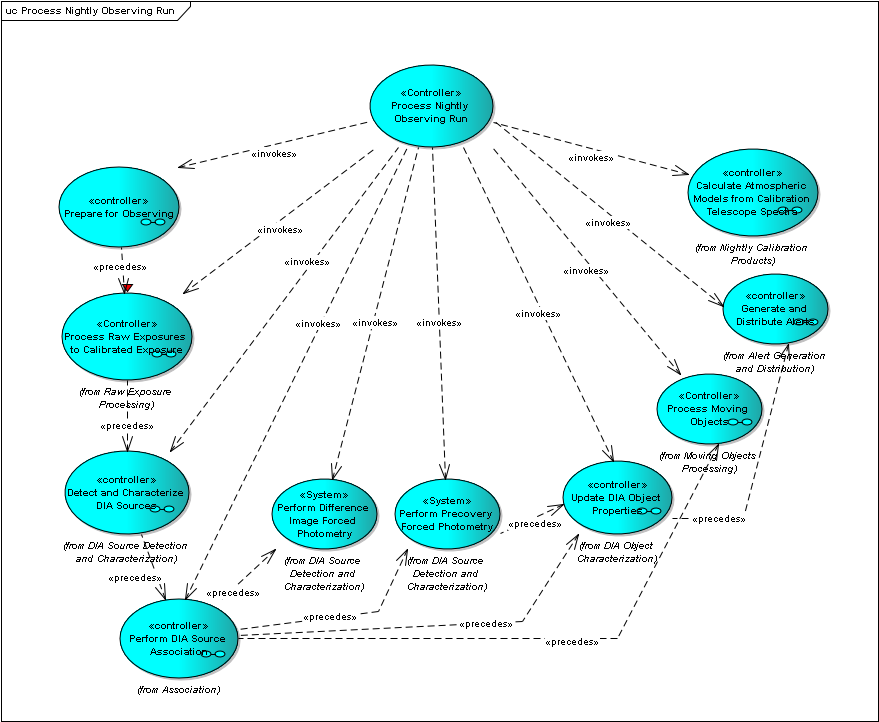
\includegraphics[angle=0,scale=0.44]{figures/process_nightly_observing_run.png}
\caption{Level 1 Processing Flow Diagram\label{fig:level1}}
\end{figure}

The logical flow of Level 1 processing is shown in the Use Case diagram presented in Figure~\ref{fig:level1}. For every observation, the following sequence of events will unfold:
%
\begin{enumerate}
\item A visit is acquired (\uc{Prepare for Observing}) and reduced (\uc{Process Raw Exposures to Calibrated Exposure}) to a single {\em visit image}. This includes instrumental signature removal\footnote{E.g., subtraction of bias and dark frames, flat fielding, bad pixel/column interpolation, etc.}, combining of snaps, etc.
  % RHL I removed cosmic ray rejection as it's not clear if it's in ISR or snap combination.

\item The visit image is differenced against the appropriate template and \DIASources are detected (\uc{Detect and Characterize DIA Sources}). If necessary, deblending is performed at this stage.

The flux and shape of the DIASource are measured on the difference image. PSF photometry is performed on the visit image at the position of the \DIASource to obtain a measure of the absolute flux.
  % RHL this is tricky in crowded fields (inc. SNe on galaxies).  We should rethink this a bit at some point.

\item The \DB is searched for a \DIAObject or an \SSObject with which to positionally associate the newly discovered \DIASource. If no match is found, a new \DIAObject is created and the observed \DIASource is associated to it.

If the \DIASource has been associated to an \SSObject (a known Solar System object), it will be flagged as such and an alert will be issued. Further processing will occur in daytime (\uc{Process Moving Objects}).

\item Otherwise, the associated \DIAObject measurements will be updated with new data (\uc{Update DIA Object Properties}). All affected columns will be recomputed, including proper motions, centroids, light curves, nearest Level 2 \Objects, etc.
  % RHL do we really want to update e.g. the proper motion/parallax on each visit?

\item An alert is issued (\uc{Generate and Distribute Alerts}) that includes all required components, as described in the \DPDD.

\item For all \DIAObjects overlapping the field of view to which a \DIASource from this visit has \emph{not} been associated, forced photometry will be performed (\uc{Perform Difference Image Forced Photometry}).  No alerts will be issued for these measurements.

\end{enumerate}

Within 24 hours of discovery, LSST DM system will perform \emph{precovery} PSF forced photometry on any prior difference image overlapping the predicted position of new \DIAObjects taken within the past 30 days (\uc{Perform Precovery Forced Photometry}).
\\

Similarly, in daytime after the nightly observing run, atmospheric models from the calibration telescope spectra will be calculated (\uc{Calculate Atmospheric Models from Calibration Telescope Spectra}) and made available to the users.
\\

In addition to these, the Moving Object Pipeline (MOPS; \wbsMOPS; \uc{Process Moving Objects}) will also be run in daytime. It is described in its own section of this document, with a detailed design in a separate Moving Object Pipeline Design Document (\MOPSD).

\subsubsection{Level 2 Pipelines Overview}

\begin{figure}[!htbp]
    \centering
    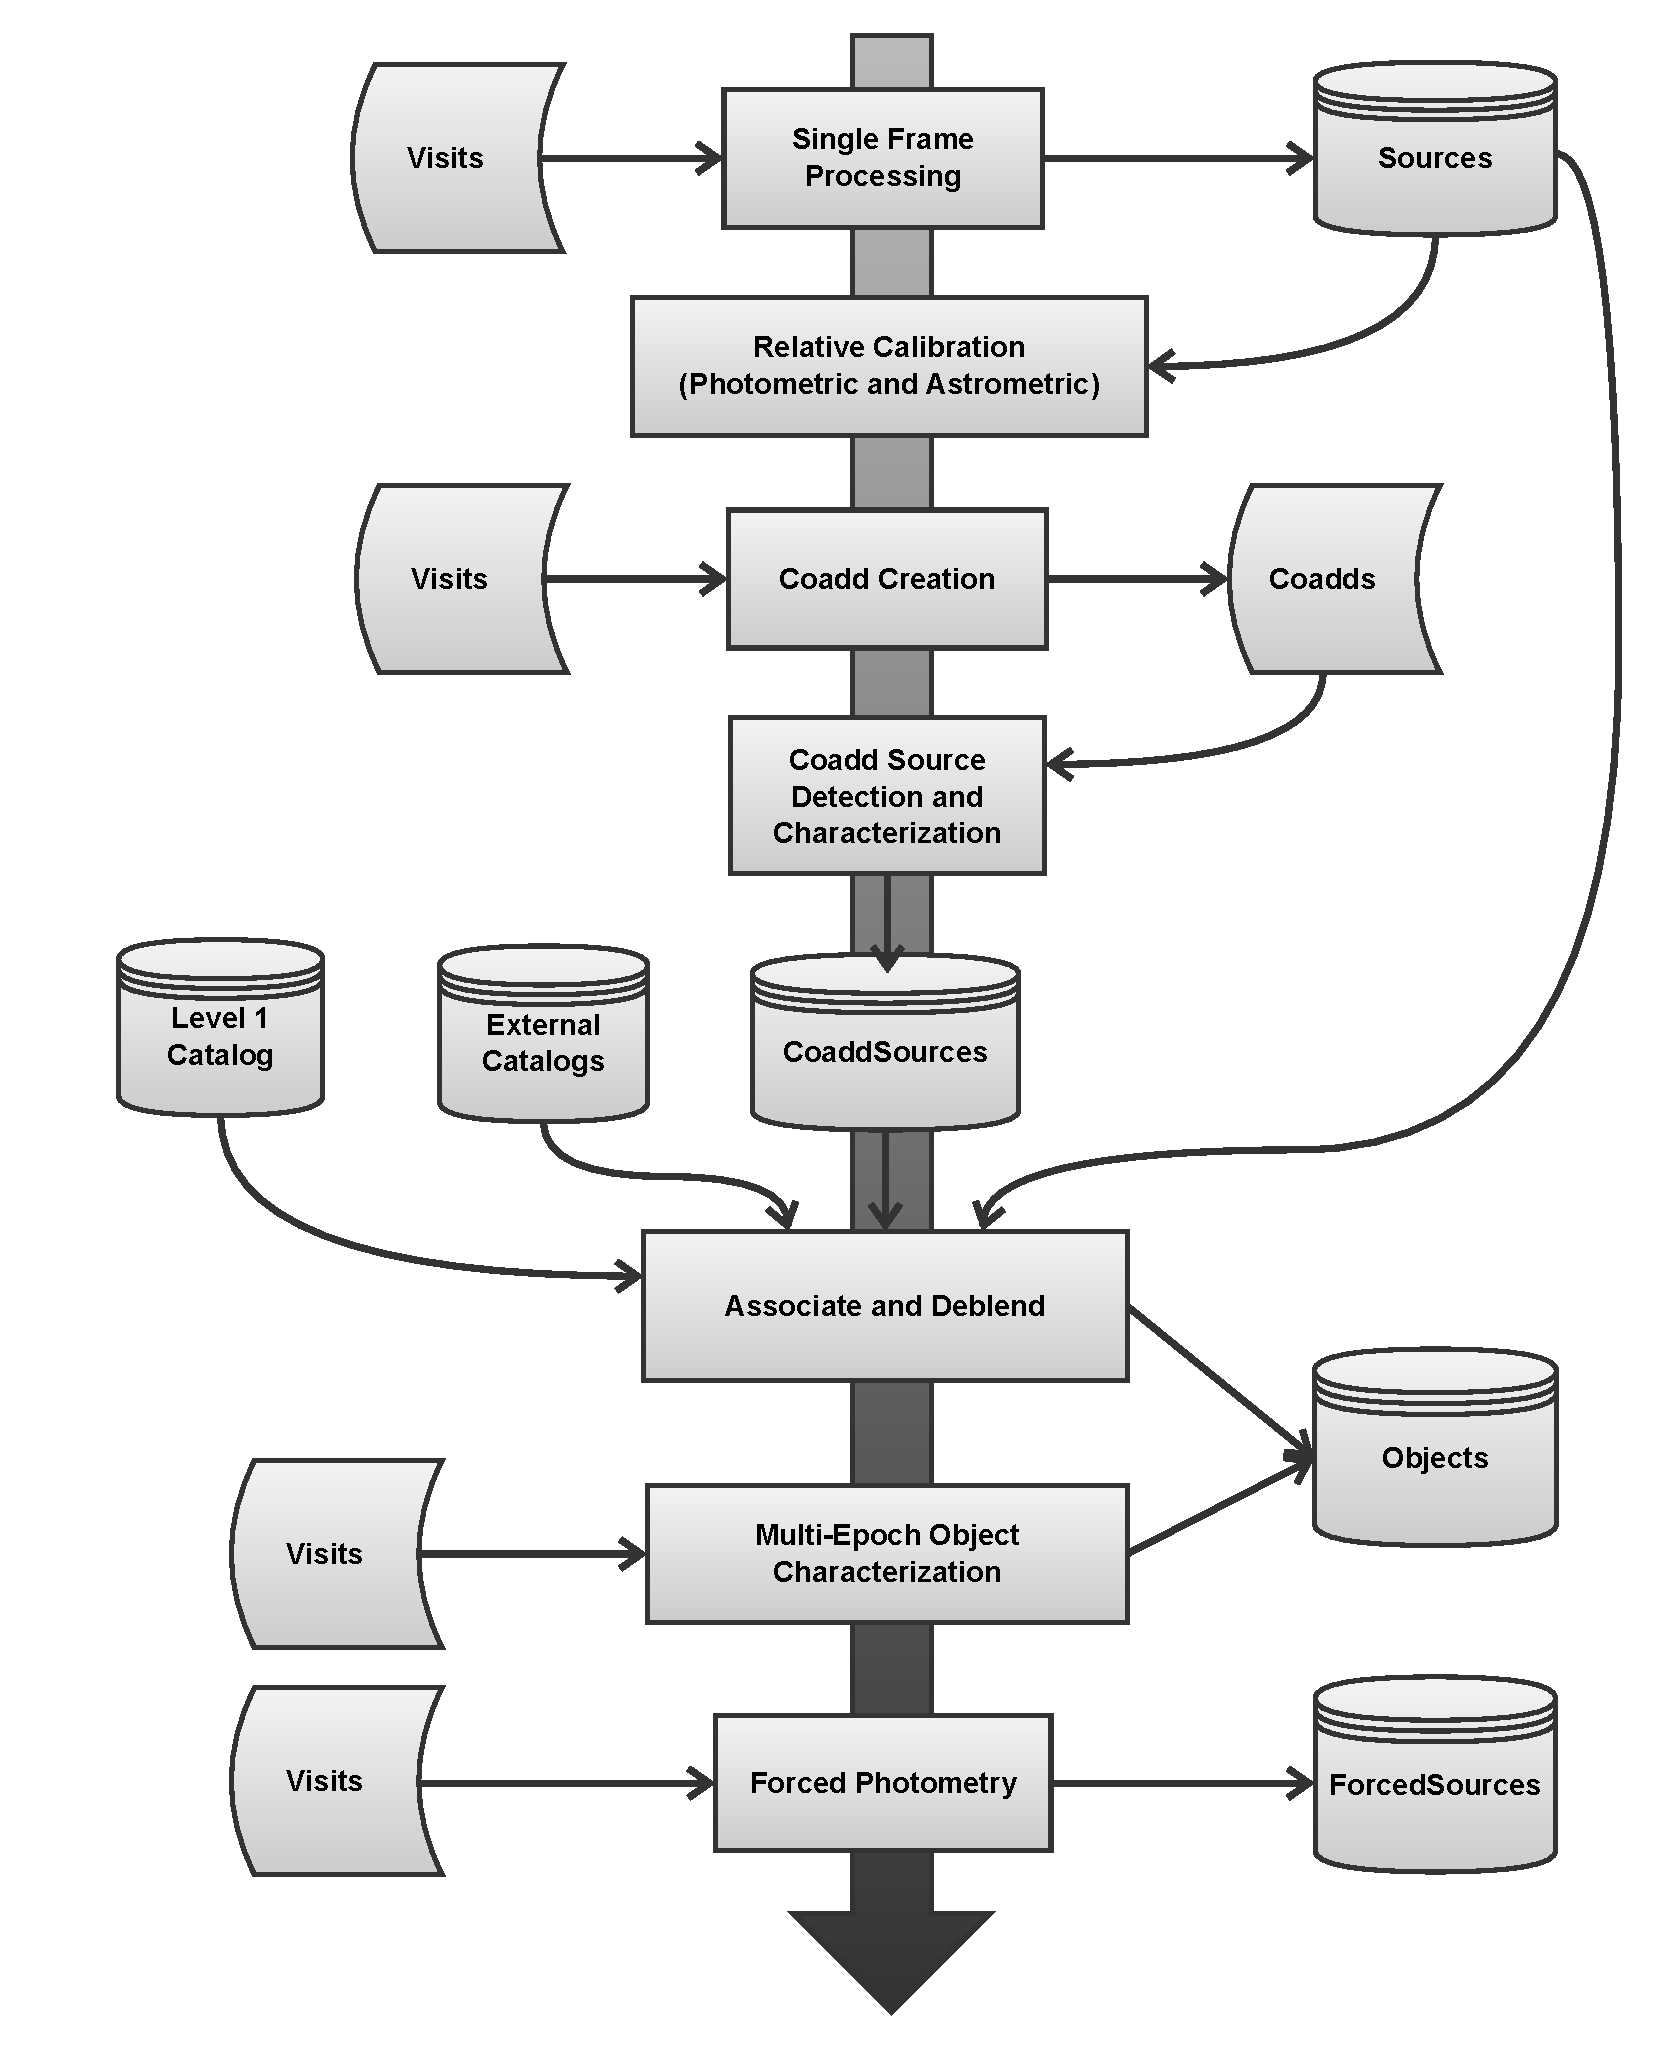
\includegraphics[scale=0.5]{figures/Level_2_Processing_Flowchart}
    \caption{Level 2 Processing Overview\label{fig:level2dp}}    
\end{figure}

Figure~\ref{fig:level2dp} presents a high-level overview of the Level 2 data processing workflow. Logically\footnote{The actual implementation may parallelize these steps to the extent possible; see LDM-230, the Automated DM Operations Document (\DMOps).}, the processing begins with single-frame (visit) image reduction and source measurement, followed by global astrometric and photometric calibration, coadd creation, detection on coadds, association and deblending, object characterization, and forced photometry measurements. The UML Use Case model (\appsUMLusecase) captures these activities in the \uc{Produce a Data Release} diagram.
\\

The following is a high-level description of steps which occur during regular Level 2 data processing:
\begin{enumerate}
    \item \emph{Single Frame Processing}: Raw exposures are reduced to \emph{calibrated visit exposures}, and \Sources are independently detected, deblended, and measured on all visits. Their measurements (instrumental fluxes and shapes) are stored in the \Source table. This step is performed by the {\bf \emph{Single Frame Processing Pipeline}} (\wbsSFM).
    \item \emph{Relative calibration}: The survey is internally calibrated, both photometrically and astrometrically using the {\bf \emph{Astrometric}} (\wbsAstroCal) and {\bf \emph{Photometric Calibration Pipelines}} (\wbsPhotoCal). Relative zero points over the focal plane and astrometric corrections are computed for every visit.
    \item \emph{Coadd creation}: Deep, seeing optimized, and short-period per-band coadds are created in $ugrizy$ bands, as well as deeper, multi-color, coadds. This task is performed by the {\bf \emph{Image Coaddition Pipeline}} (\wbsCoadd). Transient sources (including Solar System objects, explosive transients, etc), will be rejected from the coadds.
    \item \emph{Coadd source detection}. Sources will be detected on all coadds generated in the previous step. The source detection algorithm will detect regions of connected pixels, known as \emph{footprints}, above the nominal $S/N$ threshold in the \emph{PSF-likelihood image} of the visit. Each footprint may have one or more \emph{peaks}, and the collection of these peaks (and their membership in the footprints) are the output of this stage. This information will be stored in a catalog of \CoaddSources. The detection is performed by the {\bf \emph{Object Detection and Deblending}} system (\wbsDetDeblend).
    \item \emph{Coadd source deblending and characterization}. The next stage in the pipeline will decompose the \CoaddSources into a set of individual astronomical sources which is consistent across all bands, a process known as \emph{deblending}. The deblender may make use of the catalogs of \Sources and \CoaddSources, catalogs of \DIASources, \DIAObjects and \SSObjects detected on difference images, and objects from external catalogs. The deblended objects will then be characterized by measuring their positions, shapes and fluxes on the coadded images and by fitting galaxy models. This functionality is contained within the {\bf \emph{Object Detection and Deblending}} system (\wbsDetDeblend) and the {\bf \emph{Object Characterization Pipeline}} (\wbsObjChar).
    \item \emph{Multi-epoch object characterization}. A set of measurements (including predefined classes of model fits) will be performed on each of the \Objects identified in the previous step, taking all available multi-epoch data into account. Model fits will be performed using \emph{MultiFit}-type algorithms. Rather than coadding a set of images and measuring object characteristics on the coadd, MultiFit simultaneously fits PSF-convolved models to the objects multiple observations. This reduces systematic errors, improves the overall $S/N$, and allows for fitting of time-dependent quantities degenerate with shape on the coadds (for example, the proper motion). The models we plan to fit will \emph{not} allow for flux variability. Object characterization is a part of the {\bf \emph{Object Characterization Pipeline}} (\wbsObjChar).
    \item \emph{Forced Photometry}. Source fluxes will be measured on every visit, with the position, motion, structural parameters, and deblending characterized in the previous step kept fixed.
      % RHL we're not clear about which model we'll use for this forced photometry. The best-fit Sersic? 
      This process of \emph{forced photometry}, will result in the characterization of the light-curve for each object in the survey. Forced photometry is functionally a part of the {\bf \emph{Object Characterization Pipeline}} (\wbsObjChar).
\end{enumerate}


% \subsubsection{Calibration Pipelines}

\subsubsection{Enabling Level 3 Pipelines}

Level 3 capabilities are envisioned to enable science cases requiring further custom user-specified processing, especially the kind that would greatly benefit from co-location within the LSST Data Access Center. The high-level requirement for Level 3 is established in \S 3.5 of the LSST SRD.

To enable Level 3 use cases, LSST Data Management pipelines will be designed in a modular fashion to maximize the potential for reusability and synergy between Level 3 and Levels 1 and 2.

For example, a typical Level 3 use case will be to perform a different kind of measurement on objects detected in the course of Level 2 processing. A user will be able to do this by reusing the desired components of Level 2 processing, plugging in (via Python {\tt import} directives in the appropriate configuration file) the modules for their custom measurement, and executing the pipeline. The {\bf \emph{Science Pipeline Toolkit}} (\wbsSPT) will provide the necessary components to support user-driven construction and execution of custom pipelines.

\subsubsection{Science Data Quality Analysis Pipeline and Toolkit}

Science Data Quality Analysis requirements are described in the Data Quality Assurance Plan (\SDQAP) document. They will be implemented by the {\bf \emph{SDQA Pipeline}} (\wbsSDQAP; the data collection backend) and the {\bf \emph{SDQA Toolkit}} (\wbsSDQAT; the data analysis front-end).
\\

LSST QA will include four main components, which to some extent reflect the Level 1-3 structure of LSST data products. Level 0 QA is software development related, Level 1 QA relates to nightly operations, Level 2 QA relates to data releases, and Level 3 QA is science based.

\begin{itemize}
    \item {\bf Level 0 QA} includes the extensive and thorough testing of the DM subsystem during the pre-commissioning phase, as well as the tests of software improvements during the commissioning and operations phases (regression tests based on pipeline outputs and input truth). A common feature of Level 0 QA is the use of LSST simulations products, or any other dataset where the truth is sufficiently well known (e.g., the use of high-resolution observations from space telescopes to test resolved/unresolved object separation algorithms). The main goal of Level 0 QA is to quantify the software performance against these known expected outputs (e.g., to measure the completeness and false positive rate for an object finder; to measure the impact of blended sources on pipeline outputs; to measure the performance of calibration pipelines and MOPS), and to test for algorithm implementation problems (a.k.a. “coding bugs”).
    
    \item {\bf Level 1 QA} assesses the system status and data quality in real time during commissioning and operations. Its main difference from other observatory, telescope, and camera status reporting tools will be heavy reliance on the massive science imaging data stream (in addition to various telemetry and metadata generated by the subsystems). This level is tasked with nightly reporting of the overall data quality, including the nightly data products (difference images and transient source event stream) and calibration products. Real-time information about observing conditions, such as sky brightness, transparency, seeing, and about the system performance, such as the achieved faint limit, will be delivered by Level 1 QA\@. Because the actual science data stream will be analyzed, Level 1 QA tools will be in a good position to discover and characterize subtle deterioration in system performance that might not be easily caught by tools employed by the telescope and the camera subsystems for self-reporting purposes.

    \item {\bf Level 2 QA} assesses the quality of data products scheduled for the Data Releases, and provides quantitative details about data quality for each release (including the co-added image data products, and the properties of astrometrically and photometrically variable objects). This level also performs quality assessment for astrometric and photometric calibration, as well as for derived products, such as photometric redshifts for galaxies
      % RHL are we responsible for photo-z quality?  I thought it was Level 3
      and various photometric estimators for stars. Subtle problems with the image processing pipelines and systematic problems with the instrument will be discovered with Level 2 QA.
    
    \item {\bf Level 3 QA} quality assessment will be based on science analysis performed by the LSST user community. LSST will not develop Level 3 QA tools, but Level 0-2 visualization and data exploration tools will be made available to the community to form a basis on which Level 3 tools can be built. Common features expected for tools at this level are sensitivity to subtle systematic issues not recognized by Level 2 QA, and feedback about data quality to the project by external teams. It is envisioned that especially useful Level 3 QA tools would be migrated to Level 2 QA.

\end{itemize}


\section{Alert Production}
\label{sec:ap}



Alert Production is run each night to produce catalogs and images for sources that have varied or moved relative to a previous observation.  The data products produced by Alert production are given in  \hyperref[table:ap_data_products]{Table~\ref{table:ap_data_products}}.


\begin{table}[htb]
\small
\begin{tabularx}{\textwidth}{ | l | l | X | }
  \hline
  \textbf{Name} & \textbf{Availability} & \textbf{Description} \\
  \hline
  \DIASource & Stored &
  Measurements from difference image analysis of individual exposures. \\
  \hline
  \DIAObject& Stored &
  Aggregate quantities computed by associating spatially colocated \DIASources. \\
  \hline
  DIAForcedSource & Stored &
  Flux measurements on each difference image at the position of a \DIAObject. \\
  \hline
  \SSObject & Stored &
  Solar system object derived by associating \DIASources and inferring their orbits. \\
  \hline
  CalExp & Stored &
  Calibrated exposure images for each CCD/visit (sum of two snaps) and associated metadata (e.g.\ WCS and estimated background). \\
  \hline
TemplateCoadd & Temporary &
  DCR corrected template coadd. \\
  \hline
  DiffExp & Stored &
  Difference between CalExp and PSF-matched template coadd. \\
  \hline
  VOEvent & Stored &
  Database of VOEvents as streamed from the Alert Production\\
  \hline
 Tracklets & Persisted &
  Intermediate data product for the generation of \SSObjects generated by linking moving sources within a given night \\
  \hline



  \hline
\end{tabularx}
\caption{Table of derived and persisted data products produced during  Alert Production.  A detailed  description of these data products can be found in the Data Products Definition Document \citedsp{LSE-163}.
\label{table:ap_data_products}}
\end{table}

Alert Production is designed as five separate components: single frame processing, alert generation, alert distribution, precovery photometry, and a moving objects pipeline. The first four of these components run as a linear pass through of the data. The moving objects pipeline is run independently of the rest of the alert production. The flow of information through this system is shown in \hyperref[fig:nightly]{Figure~\ref{fig:nightly}}.

\begin{figure}
\begin{center}
\includegraphics[width=0.9\textwidth]{figures/LDM-151_Nightly_Overview.png}
\caption{\label{fig:nightly} The alert production flow of data through the processing pipelines (single frame processing, alert generation,  alert distribution, precovery photometry) }
\end{center}
\end{figure}

In this document we do not address estimation of the selection function for alert generation through the injection of simulated sources. Such a process could be undertaken in batch mode as part of the DRP. Source detection thresholds can be estimated through the use of sky sources (PSF photometry measurements positioned in areas of blank sky).

\subsection{Single Frame Processing Pipeline (\wbsSFM)}
\label{sec:apSingleFrameProcessing}

The Single Frame Processing (SFM) Pipeline (see Figure~\ref{fig:apSFM}) is responsible for reducing raw or camera-corrected image data to \emph{calibrated exposures}, the detection and measurement of \Sources (using the components functionally  part of the Object Characterization Pipeline), the characterization of the point-spread-function (PSF), and the generation of an astrometric solution for an image. Calibrated exposures produced by the SFM pipeline must possess all information necessary for measurement of source properties by single-epoch Object Characterization algorithms.

Astrometric and photometric calibration requires the detection and measurement of the properties of \Sources on a CCD. Accurate centroids and fluxes for these \Sources require an estimation of the PSF and background, which in turn requires knowledge of the positions of the \Sources on an image. The SFM pipeline will, therefore, iterate over background estimation (see \ref{sec:apPSFBackground}) and source measurement (see \ref{sec:apSourcemeasurement})

The SFM pipeline will be implemented as a flexible framework where new processing steps can be added without modifying the stack code (this would include the ability to process non-crosstalk corrected images should a network outage between the base and processing center result in  only the raw data being available). The pipeline, or a subset of the pipeline, should be capable of being run at the telescope facility during commissioning and operations.

\begin{figure}[th]
\begin{center}
\includegraphics[width=0.9\textwidth]{figures/SFM.png}
\caption{\label{fig:apSFM} Single frame processing of the nightly data: instrument signature removal, astrometric and photometric calibration, background and PSF estimation from the cross-talk corrected camera images.}
\end{center}
\end{figure}

%SFM pipeline functions include:
%\begin{itemize}
%\item Assembly of per-amplifier images to an image of the entire CCD;
%\item Instrumental Signature Removal;
%\item Cosmic ray rejection and snap combining;
%\item Per-CCD determination of zeropoint and aperture corrections;
%\item Per-CCD PSF determination;
%\item Per-CCD WCS determination and astrometric registration of images;
%\item Per-CCD sky background determination;
%\item Source detection and measurement on single frame images
%\item Generation of metadata required by the OCS
%\end{itemize}

\subsubsection{Input Data}
\label{sec:apSFMinput}

\paragraph*{Raw Camera Images:} Amplifier images that have been corrected for crosstalk and bias by the camera software. All images from a visit should be available to the task (including snaps). An approximate WCS is assumed to be available as metadata derived from the Telescope Control System with an absolute pointing uncertainty (for a full focal plane) of 2 arcseconds \ossreq{0298}\reqparam{absPointErr} and the field rotation known to an accuracy of 32 arcseconds \citedsp{LTS-206}.
%\begin{draftnote}
%  question into Steve R about Camera operations - DM to provide request for operations on images that camera team will undertake
%\end{draftnote}

\paragraph*{Reference Database:} A full-sky astrometric and photometric reference catalog of stars derived either from an external dataset (e.g.\ Gaia) or from the Data Release Processing. Given the current Gaia data release timeline the initial reference catalog is expected to have an astrometric uncertainty of $<0.5$ milliarcseconds and a photometric uncertainty of $<$20 millimag (for a $V=19$ G2V star). The expected release of these calibration catalogs is 2018 and will be derived from the Gaia spectrophotometric observations of non-variable sources.

\paragraph*{Calibration Images:} Flat-field calibration images for all passbands and all CCDs appropriate for the time at which the observations were undertaken. No corrections will be made in the flat-fields for non-uniform pixel sizes - the flat-fields will correct to a common  surface brightness. A flat SED will be assumed for all flat field corrections. Fringe frame calibration images scaled to an amplitude derived from the sky background (i.e.\ no sky spectrum will be available).

\paragraph*{Image Metadata:} List of the positions and extents of CCD defects for all CCDs within the focal plane; electronic parameters for all CCDs (saturation limits, readnoise parameters), electronic and physical footprint for the CCDs, linearity functions, models for the variation in the PSF width with source brightness (brighter-fatter), and parameterized models for a component-based  WCS (e.g.\ a series of optical distortion models) as needed.

\subsubsection{Output Data}
\label{sec:apSFMoutput}

\paragraph*{CalExp Images:} A calibrated exposure (CalExp) is an \hyperref[sec:spImagesExposure]{Exposure} object. The CalExp contains the image pixel values, a variance image, a bitwise mask, a representation of the PSF, the WCS (possibly decomposed into separable components), a photometric calibration object, and a model for the  background. For the alert production, it is not anticipated that a model of the per-pixel covariance will be persisted but this will be revisited dependent on the performance of image subtraction and anomaly characterization as described in \ref{sec:apAlertGeneration}.

\paragraph*{Source Databases:} A catalog of \Sources with measured features described in \ref{sec:apSourcemeasurement}.

\paragraph*{OCS Database} A parameterization of the PSF, WCS, photometric zeropoint, and depth for each CCD in a visit. The PSF may be a simplified version (e.g.\ a single Gaussian) of that derived for the Alert production. These data will be made available to the Telescope Control System (TCS) to assess the success of each observation. A limited version of nightly SFM could be run on the summit to generate this information or the  data will be persisted within a database at the data center that will be accessible to the TCS.


\subsubsection{Instrumental Signature Removal}
\label{sec:apISR}
Instrumental Signature Removal characterizes, corrects, interpolates and flags the camera (or raw) amplifier images to generate a flat-fielded and corrected full CCD exposure.

\paragraph{Pipeline Tasks}
\begin{itemize}
\item Mask the image defects at the amplifier level based on the CCD defect lists, and the per CCD saturation limits
\item Assemble the amplifiers into a single frame (masking missing amplifiers)
\item Apply full frame corrections: dark current correction, flat field to preserve surface brightness, fringe corrections. Flat fields will assume a flat spectral energy distribution (SED) for the source. Fringe frames will be normalized by fitting to the observed sky background.
\item Apply pixel level corrections: apply a correction model for brighter-fatter to homogenize the PSF, correct for static pixel size effects based on a model
\item Interpolate across defects and saturated pixels assuming a model for the PSF (with a nominal FWHM). An estimate of the PSF will be needed for this operation (from the TCS/OCS) or interpolation may be needed to be performed at the end of \ref{sec:apPSFBackground}.
\item Apply a cosmic ray detection algorithm as described in \ref{sec:acCosmicRayDetection}
\item Generate a summed and difference image from the individual snaps propagating the union of the mask pixels in each snap
\end{itemize}

Dependent on the properties of the delivered LSST image quality for 15 second snaps it may be required to model any bulk motion between snaps prior to combination (e.g.\ if dome seeing or the ground layer dominate the lower order components of the seeing).

\subsubsection{PSF and background determination}
\label{sec:apPSFBackground}

Given exposures that have been processed through Instrument Signature Removal, \Sources must be detected to determine the astrometric and photometric calibration of the images. As noted previously an iterative procedure will be adopted to generate an estimate of the background and PSF, and to characterize the properties of the detected sources.  Convergence criteria for this procedure are not currently defined. The default implementation assumes three iterations.

\paragraph{Pipeline Tasks}

The iterative process for PSF and background estimation comprises,
\begin{itemize}
\item Background estimation on the scale of a single CCD is as described in \ref{sec:acBackgroundEstimation}, which divides the CCD into subregions and estimates the background using a robust mean from non-source pixels.
\item Subtraction of the background and the detection of sources as described in \ref{sec:acSourceDetection}. The initial detection threshold for source detection will be 5$\sigma$, with $\sigma$ estimated from variance image plane.
\item Measurement of the properties of the detected sources (see \ref{sec:apSourcemeasurement}). Dependent on the density of sources it may be necessary to deblend the images as described in \ref{sec:acDeblending}
\item Selection of isolated PSF candidate stars based on a signal-to-noise threshold (default 50 $\sigma$). This threshold is significantly deeper than the magnitude limit for Gaia astrometric catalogs but is the threshold at which the astrometric error on the centroid due to photon noise is less than 10 mas and the photometric noise is less than 2\% for the case of the use of a deeper DRP derived reference catalog.
\item Single CCD PSF determination using the techniques described in \ref{sec:acSingleCCDPSF} and the selected bright sources
\item Masking of source pixels within the CCD (growing the footprint of the \Sources to mask the outer regions of the \Source profiles will likely be required to exclude contributes to the background from low surface brightness features).
%\item Single CCD \hyperref[sec:acModelSpatialPSF]{PSF spatial model}
\end{itemize}

The default expectation is that all tasks within this procedure would iterate until convergence.  There maybe significant speed optimizations to be gained by excluding the \Source detection step after an initial detection if the number of sources does not change significantly with updates to the background model.
%\begin{draftnote}
%  Treatment of covariance
%\end{draftnote}

\subsubsection{Source measurement}
\label{sec:apSourcemeasurement}

For the \Source catalog generated in \ref{sec:apPSFBackground}, source properties are measured using a subset of features described in \ref{sec:acMeasurement}. Source measurement is for all sources within the \Source catalog and not just the bright subset used to calibrate the PSF.  We anticipate using the following plugin algorithms within the \Source measurement step,
\begin{itemize}
\item Centroids based on a static PSF model fit (see \ref{sec:acCentroidAlgorithms} and \ref{sec:acStaticPointSourceModels})
\item Aggregation of pixel flags as described in \ref{sec:acPixelFlags}
\item Aperture Photometry as geven in \ref{sec:acAperturePhotometry} (but only for one or two radii)
\item PSF photometry given in \ref{sec:acStaticPointSourceModels} assuming a static PSF model fit
\item  An aperture correction estimated assuming a static PSF model and measurement of the curve of growth for  detected sources as given in \ref{sec:acApCorr}
\end{itemize}
%\begin{draftnote}
%  why only one or two radii
%\end{draftnote}

\subsubsection{Photometric and Astrometric calibration}

Photometric and astrometric calibration entails a ``semi-blind'' cross match (because the pointing of the telescope is known to an accuracy of 2 arcseconds) of a reference catalog derived either from the DRP \Objects or from an external catalog (see \ref{sec:apSFMinput}), the generation of a WCS (on the scale of a CCD or full focal plane), and the generation of a photometric zeropoint (on the scale of a CCD). These algorithms must degrade gracefully for the case of larger pointing errors (e.g.\ during the initial calibration of the system during commissioning) and may need to operate in a ``blind'' mode where the pointing and orientation of the telescope is not known.

\paragraph{Pipeline Tasks}

The photometric and astrometric calibration is expected to be performed at the scale of a single CCD. It is possible that the calibration process will need to be extended to larger scales (up to a full focal plane) if there is significant structure in the photometric zero point, or if astrometric distortions cannot be calibrated at the scale of the CCD with sufficient accuracy (i.e.\ the astrometric distortions do not dominate the false positives in the image subtraction). A full focal plane level calibration strategy will introduce synchronization points within the processing of the CCDs as the detections on all CCDs will need to be aggregated prior to the astrometric fit.

The procedures used to match and calibrate the data are,
\begin{itemize}
\item CCD level source association between the DRP reference catalog (or external catalog) and \Sources detected during the PSF and background estimation stage will use a simplified Optimistic B approach described in \ref{sec:acSingleCCDReferenceMatching}. Given an astrometric accuracy of $<0.5$ milliarcseconds from external catalogs such as Gaia (for a $V=19$ G2V star) or  an accuracy of $<50$ milliarcseconds for the DRP catalogs the search radii for sources will be dominated by the uncertainties in the pointing of the telescope and the rotation angle of the camera.
\item Generation of a photometric solution on the scale of a single CCD as described in \ref{sec:acSingleCCDPhotometricFit}
\item Fitting of a WCS astrometric model for a single CCD  using the algorithms given in \ref{sec:acSingleCCDAstrometricFit}. The WCS model is expected to be composed of a sum of transforms or astrometric components (e.g.\ a optical model for the telescope, a lookup table or model for sensor effects such as tree rings).
\item Persistance of the astrometric, PSF, and photometric solutions for possible use by the Telescope Control system (TCS) (see \ref{sec:apSFMoutput})
\end{itemize}

Given the number of stars available on a CCD or the complexity of the astrometric solutions for the LSST (e.g.\ the decomposition of the WCS into components) it may be necessary that the astrometric and photometric solutions be performed for a full focal plane and not just a CCD.  For these cases the algorithms used will be single visit matching (see \ref{sec:acSingleVisitReferenceMatching}),  single visit photometric solutions (see \ref{sec:acSingleCCDPhotometricFit}), and single visit astrometric fits (see \ref{sec:acSingleVisitAstrometricFit}). Fitting to a full focal plane introduces a synchronization point in the alert processing where all CCDs must have completed their previous processing steps prior to the astrometric calibration.

Astrometric and photometric solutions  within crowded fields will utilize the bright and easily isolated sources within a CCD image. The order of the WCS used in the astrometric fits will, therefore, depend on the number of calibration \Sources that are available.

\subsection{Alert Generation Pipeline (\wbsDiffim)}
\label{sec:apAlertGeneration}

The Alert Generation pipeline identifies variable, moving, and transient sources within a calibrated exposure by subtracting a deeper template image (see Figure~\ref{fig:apAlertgen}). The \DIASources detected on a DiffExp are associated with known \DIAObjects and \SSObjects (that have been propagated to the date of the CalExp exposure) and their properties measured. The process for image differencing requires the creation or retrieval of a TemplateCoadd, the matching of the  astrometry and PSF of the TemplateCoadd to a CalExp, and subtracting the template image from the CalExp. Spurious \DIASources will be removed using morphological and environment based classification algorithms.

The Alert Generation pipeline is required to difference, and detect and characterize \DIASource sources within 24s (allowing for multiple cores and multithreading of the processing).
%The requirement on the algorithms for purity and completeness of the sample is given by the \DMSR\@. Image differencing shall perform as well in crowded as in uncrowded fields.


\begin{figure}[th]
\begin{center}
\includegraphics[width=0.9\textwidth]{figures/Alert_Generation.png}
\caption{\label{fig:apAlertgen} Generation of alerts from the nightly data: image differencing and measurement of the properties of the \DIASources, identification and filtering of spurious events, association of previously detected \DIAObjects and \SSObjects with the newly detected \DIASources. }
\end{center}
\end{figure}
\subsubsection{Input Data}
\label{sec:apAGInput}

\paragraph*{CalExp Images:} Calibrated exposure processed through \ref{sec:apSingleFrameProcessing} with associated WCS, PSF, mask, variance, and background estimation.

\paragraph*{Coadd Images:} TemplateCoadd images that spatially overlap with the CalExp images processed through \ref{sec:apSingleFrameProcessing}. This coadded image is optimized for image subtraction and is expected to be characterized in terms of a tract/patch/filter. Generation of this template may account for differential chromatic refraction or be generated for a limited range of airmass, seeing, and parallactic angles.

\paragraph*{Object Databases:} \Objects that spatially overlap with the CalExp images processed through \ref{sec:apSingleFrameProcessing}. This \Object catalog will provide the source list for determining nearest neighbors to the detected \DIASources.


\paragraph*{DIAObject Databases:} \DIAObjects that spatially overlap with the CalExp images processed through \ref{sec:apSingleFrameProcessing}. This \DIAObject catalog will provide the association  list against which the \DIASources will be matched.

\paragraph*{SSObject Databases:} The \SSObject list at the time of the observation. The \SSObject positions will be propagated to the date of the CalExp observations and will provide an association  list for cross-matching against the detected \DIASources to identify known Solar System objects.

\paragraph*{Reference classification catalogs:} Classification of \DIASources based on their morphological features (and possibly estimates of the local density or  environment associated with the \DIASource) will be undertaken prior to association in order to reduce the number of false positives. The data structures that define these classifications will be required as an input to this spuriousness analysis.



\subsubsection{Output Data}
\label{sec:apAGOutput}

\paragraph*{DiffExp Images:} Image differences derived by subtracting a TemplateCoadd from a CalExp image.

\paragraph*{DIASource Databases:} \DIASources detected and measured from the DiffExps using the set of parameters described in \DPDD will be persisted.


\paragraph*{DIAObject Databases:} \DIASource will be associated with existing \DIAObjects and persisted. New \DIASource (i.e.\ those not associated) will generate a new instance of a \DIAObject.


\subsubsection{Template Generation}
\label{sec:apCRTemplates}

Template generation requires the creation or retrieval (see \ref{sec:acRetrieveTemplate}) of a TemplateCoadd that is matched to the position and spatial extent of the input CalExp. Generation of the TemplateCoadd could be from a persisted Coadd that was generated from CalExp exposures with comparable (within a predefined tolerance) airmass and parallactic angles, or from a model that corrects for the effect of  differential chromatic refraction (see \ref{sec:acDCRTemplates}). It is expected that these operations would be undertaken on a CCD level but for efficiency the TemplateCoadd might be returned for a full focal plane or a series of \textit{patches}  or a \textit{tract}.


\paragraph{Pipeline Tasks}

\begin{itemize}
\item Query for a TemplateCoadd images that are within a given time interval of the CalExp  (default 2 years) of the current CCD image, and are within a specified airmass and parallactic angle.
\item (optional) Derive a seeing and DCR corrected TemplateCoadd from a model (see DCR template generation in \ref{sec:acDCRTemplates}). The current prototype approach assumes that the TemplateCoadd  will be derived for the zenith and will comprise a data cube with spatial and wavelength dimensions (a low resolution spectrum per pixel). Propagating to the observation will require aligning the DCR correction in the direction of the parallactic angle of the CalExp.
\end{itemize}

\subsubsection{Image differencing}

Image differencing incorporates the matching of a TemplateCoadd to a CalExp (astrometricly and in terms of image quality), subtraction of the template image, detection and measurement of \DIASources, removal of spurious \DIASources, and association of the \DIASources with previously identified \DIAObjects, and \SSObjects.

\paragraph{Pipeline Tasks}

\begin{itemize}
\item Determine a relative astrometric solution from the WCS of the TemplateCoadd image and CalExp image
\item Match the DRP \Sources for the TemplateCoadd (see \ref{sec:drpFinalImChar}) against \Sources from the SFM pipeline (see \ref{sec:apSingleFrameProcessing}) of the raw images.
\item Warp or resample the TemplateCoadd using a Lanczos filter  (as described in \ref{sec:spWarp}) to match the astrometry of the CalExp. It is possible that astrometricly matching the TemplateCoadd and CalExp using faint source will need to be undertaken dependent on the accuracy of the WCS.
\item For CalExp images with an image quality that is better than the TemplateCoadd preconvolve the CalExp image with the PSF. Use a  convolution kernel (see \ref{sec:spKernels}) that is matched to the source detection kernel. This reduces the need for deconvolution in the PSF matching (see \ref{sec:acImageSubtraction})
\item Match the PSF of the CalExp and TemplateCoadd images as described in \ref{sec:acDiffImDecorrelation} and construct a spatial model for the matching kernel. This approach may include matching to a common PSF through homogenization of the PSF (see \ref{sec:acPSFHomogenization}.
\item Apply the matching kernel to the TempCoadd and subtract the images to generate a DiffExp (as described in \ref{sec:acImageSubtraction}). Dependent on the relative signal-to-noise in the science and template image decorrelation of the template image due to the convolution of the template with a matching kernel may be necessary (see \ref{sec:acDiffImDecorrelation})
\item Detect \DIASources on the DiffExp using the algorithms described in \ref{sec:acSourceDetection}. Convolution with a detection kernel will depend on whether the CalExp was preconvolved in item 4.
\item Measurements of the \DIASources on the DiffExp will include dipole models and trailed PSF models (see  \ref{sec:acDipoleModels} and \ref{sec:acTrailedPointSourceModels} and parameters described in Table~2 of the \DPDD . The specific algorithms used for measurement of \DIASources will depend on whether the CalExp image was preconvolved.
\item Measurement of the PSF flux on snap difference images for all \DIASources.
\item The application of spuriousness algorithms, also known as ``real-bogus'', may be applied at this time dependent on whether the number of false positives is less than 50\% of the detected sources \reqparam{mopsPurityMin} \ossreq{0354} (see \ref{sec:acSpuriousnessAlgorithms})\footnote{The requirement for a 50\% false positive rate is given in the \OSS (when discussing Solar System Object requirements) and impacts the sizing model for the alert stream}. \DIASources classified as spurious at this stage may not be persisted (dependent on the density of the false positives). The default technique will be based on a trained random forest classifier. It is likely that the training of this classifier will need to be conditioned on the image quality and airmass of the observations.
\end{itemize}

\subsubsection{Source Association}
\label{sec:apSourceAssoc}

In Source Association \DIASources detected within a given CCD will be cross-matched or associated (see \ref{sec:acDIAObjectGeneration}) with the \DIAObject table and the \SSObjects (whose ephemerides have been generated for the time of the current observation). The association will be probabilistic  and account for the uncertainties within the positions. The association may include flux and priors on expected proper motions for the sources. External targets (e.g.\ well localized transient events from other telescopes or instruments) can be incorporated within this component of the nightly pipeline (essentially treating external sources as additional \DIAObjects and associating them with the \DIASources) enabling either matching to \DIASources or generation of forced photometry at the position of the external source.

\paragraph{Pipeline Tasks}

\begin{itemize}
\item Generate the positions of \SSObjects that overlap a DiffExp given its observation time by propagating the \SSObject orbit (see \ref{sec:acEphemerisCalculation})
\item As described in \ref{sec:acDIAObjectGeneration} source association will be undertaken for all \DIASources. Matching will be to \DIAObjects, and the ephemerides of \SSObjects. Positions for \DIAObjects will be based on a a time windowed (default 30 day) average of the \DIASources that make up the \DIAObject. A linear motion model for parallax and proper motion will be applied to propagate the \DIAObject to the time of the observation. A probabilistic association may need to account for one-to-many and many-to-one associations.  In dense regions it may be necessary to generate joint associations across all \DIAObjects (and associated \DIASources) in the local  vicinity of a \DIASource to correct for mis-assignment from previous observations. This could include the pruning and reassignment of \DIASources between \DIAObjects. A baseline approach for nightly processing will be to select based on a maximum a posteriori estimate for the association.
\item \DIASources will be positionally matched to the nearest 3 stars and 3 galaxies in the DRP \Object database. In its simplest case the search algorithm will be a tree-based nearest neighbor search (the default radius for association is not defined) . The matched \Objects will be persisted as a measure of local environment.
\item \DIASources unassociated with a \DIAObject will instantiate a new \DIAObject.
\item The aggregate positions for the \DIAObjects will be updated based on a rolling time window (default 30 days).
\item Proper motion and parallax of the \DIAObject will be updated using a linear model as described in \ref{sec:acStellarMotionFitting}.
%It is not currently clear if there is a science case for generating proper motions and parallaxes within the %DIAObjects if the DRP Objects are available for each source.
\end{itemize}


\clearpage

\subsection{Alert Distribution Pipeline (\wbsAP)}

The Alert Distribution Pipeline takes the newly discovered \DIAObjects (including their associated historical observations) and all related metadata as described in the \DPDD, and delivers alert packets in \VOEvent format to a variety of endpoints via standard IVOA protocols (eg., \VOEvent Transport Protocol; VTP\@). Packaging of the event will include the generation of postage stamp cutouts (30x30 pixels on average) for the difference image and the template image together with the variance and mask pixels for these cutouts.

The \SRD requires that the design of the LSST alert system should be able to handle 10$^7$ events per night, which corresponds to 10$^4$ alerts per visit or 50 alerts per CCD (with the time between subsequent visits averaging 39 seconds). All alerts (up to 10$^4$ per visit) must be transmitted within 60s of the closure of the shutter of the final snap within a visit.

For a nightly event rate of 10$^7$, and assuming the schema described in Tables 1 and 2 in the \DPDD together with the generation of the postage stamp cutouts, the \VOEvents data stream is expected to amount to 650-820~GB of data per night (assuming no filtering of the data, and depending on the possibility or effectiveness of compression). This equates to an average data rate of 150-180~Mbit/sec per full alert stream. Assuming we transmit up to 40K~alerts in a peak visit within 15~seconds, the peak data rate is expected to be 1.5-1.8~Gbit/sec per full alert stream. The Alert Distribution pipeline is designed to distribute these alerts with a workflow, including the access point of external event brokers, shown in Figure~\ref{fig:apAlertDistribution}.

In addition to the full data stream the Alert Generation Pipeline will provide a basic alert filtering service. This service will run at the LSST U.S. Archive Center (at NCSA). It will enable astronomers to create filters (see  \ref{sec:apQueue}) that limit what alerts, and what fields from those alerts, are ultimately forwarded to them. These \emph{user defined filters} will be configurable with a simplified SQL-like declarative language. Access to this filtering service will require authentication by a user.

\VOEvent alerts will be persisted in an alert database as well as distributed through a message queue. The alert database (AlertDB) will be synchronized at least once every 24 hours and will be queriable by external users. The message queue that distributes the alerts is expected to have the capability  to replay events for the case of a break in the network connection between the queue and client but not to support general queries.

\begin{figure}[th]
\begin{center}
\includegraphics[width=0.9\textwidth]{figures/Alert_Distribution.png}
\caption{\label{fig:apAlertDistribution} Distribution of alerts from the nightly processing: generation of postage stamps around each detected \DIASource, distribution of the \DIAObjects as VOEvents, simple filtering of the event stream, and persistence of the events in a database.}
\end{center}
\end{figure}

\subsubsection{Input Data}
\label{sec:apADInput}

\paragraph*{DIAObject Database:} \DIAObjects, with new \DIASources, generated through image differencing will be used to create alert packets.

\paragraph*{Difference Images:} The DiffExp will be used to  generate postage stamp (cut-out) images of \DIASources within the CCD.

\paragraph*{Coadd Images:} The TemplateCoadd used in image subtraction will be used to  generate postage stamp images of the template image for \DIAObjects.


\subsubsection{Output Data}

\paragraph*{\VOEvent Database:} \VOEvents generated from the \DIAObjects and cutouts will be persisted within a database (e.g.\ a noSQL database) or object store.




\subsubsection{Alert postage stamp generation}

Creates the associated image cutouts (30x30 pixels on average) for all detect \DIAObjects (cutouts are generated from the current observation and not from historical observations).

\paragraph{Pipeline Tasks}

 \begin{itemize}
\item Extract from the DiffExp the cutout of each \DIAObject with a \DIASource detected within the current observation.  Cutout images will be scaled to the size of the \DIASource but on average will be 30x30 pixels. Variance and mask planes, WCS, background model, and associated metadata will be persisted. The prototype implementation assumes that these cutouts will be persisted as FITS images with a projection that is the  native projection of the DiffExps.

\item Extract from the TemplateCoadd  a cutout of each \DIAObject with a \DIASource detected within the current observation.  Cutout images will be identical in size and footprint as those derived from the DiffExp. Variance and mask planes, WCS, and associated metadata will be extracted with the pixel data. The prototype implementation assumes that these cutouts will be persisted as FITS imagesand that the projection will be that of  the DiffExps.
\end{itemize}

\subsubsection{Alert queuing and persistance}
\label{sec:apQueue}

The alert queue  distributes and persists \DIAObject with new \DIASources as \VOEvents through a message queue. It includes a \textit{limited} filtering interface but persists the full \VOEvents in an AlertDB. The event message stream and the AlertDB will be  synchronized at least once every 24 hours.


\paragraph{Pipeline Tasks}

\begin{itemize}
\item Publish \DIAObjects to a caching message queue (e.g.\ \href{http://kafka.apache.org}{Apache Kafka}) through the butler. The prototype implementation assumes a distributed and partitioned messaging system that uses a \href{https://en.wikipedia.org/wiki/Publish_subscribe_pattern}{publication-subscription} model for communication between clients and the queue. This model maintains feeds of messages in categories called topics. An example topic would be a \DIAObject. Whether a topic would comprise a full \DIAObject or a subset of the data remains open (passing subsets of parameters as individual topics would require that the client be able to synchronize and join topics into a full \DIAObject). For each of the 189 CCDs, approximately 50 events will be passed as messages to the messaging queuing system. The distribution of the events from a given CCD will not be synchronized with other CCDs within the focal plane (alerts from each CCD will be independently processed).

\item A consumer layer will subscribe to the  message queue and package them as \VOEvents and distribute these events to external users. To allow for network outages between the message queue and the consumer the message queue must be able to replay previous events.
\item  The consumer layer will provide a command line API to define simple queries or filters of the events (limited to querying on existing \DIAObject fields, or filtering the attributes of the \DIAObject). Web-based interfaces to the consumer layer will be developed by SUIT.
\item Filtered or the full stream of \DIAObjects will be packaged into \VOEvents and broadcast to VOEvent clients through the consumer layer
\item A full, unfiltered, VOEvent alert stream will be broadcast to the AlertDB using the consumer layer.
\item Prior to the start of the subsequent night's observations, the message queue will be flushed and synchronized with the AlertDB. It is possible to persist the message queue on longer timescale but it is a requirement hat synchronization be performed within 24 hours of the observations.
\end{itemize}

To cope with the variation in density of events as a function of position on the sky and the need for fault tolerance the message queue will need to be able to partition and replicate data. Given the 650-820~GB of data generated per night from the alert distribution, each full alert stream will require about 0.2~Gb/s average network capacity. Whether the consumer layer will instantiate a new consumer for each filter (or client) or will orchestrate the \VOEvents from a single subscription to the message queue is an open question that will depend on the expected network topology (internal and external to the data center at NCSA).

The AlertDB will have an interface that can be queried (to enable historical searches of events) including searches on other than timestamps. It is expected that the AlertDB will be a noSQL datastore (e.g.\ Cassandra).

%partitions must be ordered the same, failover must let a consumer to move to a different partion and have the messages ordered





\clearpage

\subsection{Precovery and Forced Photometry Pipeline}

The precovery and forced photometry  pipeline performs two tasks (see Figure~\ref{fig:apForcedPrecovery}). Forced PSF photometry is undertaken for all \DIAObjects that have a detected \DIASource within a, default 1 year, window of time from the observation.  Second, within 24 hours, precovery forced photometry is performed on all unassociated \DIASources within an image (i.e.\ new \DIAObjects). For each new \DIAObject, forced (PSF) photometry will be measured at the position of the source in each of the preceding  30-days of DiffExps.

Forced photometry is not required prior to alert generation. Completion of the precovery photometry is required within 24 hours of the completion of the observations. Forced and precovery can be undertaken as part of the nightly workflow if they do not impact the time required to distribute the alerts.

\begin{figure}[th]
\begin{center}
\includegraphics[width=0.9\textwidth]{figures/Forced_Precovery.png}
\caption{\label{fig:apForcedPrecovery} Forced photometry for \DIAObjects: forced photometry on a night's DiffExp for all \DIAObjects that have detected \DIASources within the last year, precovery photometry for the previous 30 days of DiffExps for new \DIAObjects}
\end{center}
\end{figure}

\begin{draftnote}[For ZI]
  I moved the precovery to a single pipeline
\end{draftnote}
\subsubsection{Input Data}

\paragraph*{Difference images:} A cache of DiffExps within a finite time interval (default 30 days) of the previous nights observations (inclusive of the previous nights data)

\paragraph*{DIAObject Database:} All \DIAObjects with a \DIASource detection within the last 12 months and all unassociated (new) \DIAObjects observed within the previous night

%\begin{draftnote}
%  We associate (measure forward) for 12 months but look back for 30 days
%\end{draftnote}

\subsubsection{Output Data}

\paragraph*{DIAForcedSource Databases:} Forced PSF photometry at the centroid (from the aggregated individual \DIASource centroids) of a \DIAObject. The forced photometry is undertaken on the current night's DiffExp for all \DIAObjects with \DIASources detected within the last year, and on the previous 30 days of DiffExp for all newly detected \DIASources.


\subsubsection{Forced Photometry on all \DIAObjects}

Generate forced (PSF) photometry on the DiffExp for all \DIAObjects that overlap with the footprint of the CCD. Forced photometry is only generated for \DIAObjects for which there has been a \DIASource detection within the last 12 months. The forced photometry is persisted in the forced photometry table in the Level 1 database. Alerts are released prior to the generation of forced photometry and forced photometry is not released as apart of an alert which means that this component of the processing is not subject to the 60 second processing requirements for nightly processing.

\paragraph{Pipeline Tasks}

\begin{itemize}
\item Extract all \DIAObjects within the Level 1 database with a detected \DIASource within the last year (including the current nights observations). This information is available from the \DIASource and \DIAObject association.
\item For the aggregate positions within the \DIAObject undertake a PSF forced measurement as described in section \ref{sec:acForcedMeasurement}
\item Update the forced photometry tables in the Level 1 database.
\end{itemize}



\subsubsection{DIAObject Forced Photometry:}

Updated forced photometry table for all new \DIAObjects


\paragraph{Pipeline Tasks}

\begin{itemize}
\item Extract from the Level 1 database all \DIAObjects that were unassociated (i.e.\ new \DIASource detections) from the previous nights reduction. Filtering of the \DIAObjects will need to account for cases where new \DIASources are observed more than once within a night (where the second or subsequent observations do not result in a new \DIAObject).
\item Extract DiffExps within a  default 30 day window prior to the observation
\item Force photometer the extracted images as described in \ref{sec:acForcedMeasurement} using a PSF model and the centroid defined in the \DIAObject
\item Update the forced photometry table within the Level 1 database
\end{itemize}
\clearpage



\subsection{Solar System Pipeline (\wbsMOPS)}
\label{sec:apMovingObjectPipeline}

The Solar System Pipeline (SSP) is responsible for generating and managing the Solar System data products. These are catalogs of Solar System objects with associated Keplerian orbits, physical properties, errors, and detected \DIASources. Quantitatively, the linking element of the pipeline shall be capable of detecting 95\% \reqparam{orbitCompleteness} of all Solar System objects that meet the criteria specified in the \OSS\@ \ossreq{0159} (i.e.\ the observations required to define an orbit). Each visit within 10 degrees of the Ecliptic will detect approximately 4,000 asteroids.

Components of the SSP are run during and separately from nightly processing (see Figure~\ref{fig:apMOPS}). The element run in nightly processing performs association of observations with known \SSObjects, and is described in \ref{sec:apSourceAssoc}. Daytime elements cluster newly detected \DIAObjects to search for candidate asteroids. The procedure is to link \DIASource detections within a night (when on-sky motion is approximately linear) into {\em tracklets}, to link these tracklets across multiple nights (into tracks), to fit the tracks with an orbital model to identify those tracks that are consistent with an asteroid orbit, to report these candidate discoveries to the Minor Planet Center (MPC), update the \SSObject table based on the discovery confirmations from the MPC, and compute the physical properties (e.g., absolute magnitudes) of objects in the \SSObject table, and auxiliary per-observation information for individual observations. By its nature this process is iterative with \DIASources being associated and disassociated with \SSObjects. It is expected that a frequency of one day for these iterations (i.e.\ the \SSObjects will be update each day) will be sufficient.

\begin{figure}[th]
\begin{center}
\includegraphics[width=0.9\textwidth]{figures/MOPS.png}
\caption{\label{fig:apMOPS} Detection and orbital modelling of moving sources within the nightly data: Tracklet generation from revisits, filtering of tracklets based on  known \SSObjects, fitting of tracks and orbits to tracklets, pruning of tracklets and \DIAObjects based on new and updated \SSObjects.}
\end{center}
\end{figure}

\subsubsection{Input Data}

\paragraph*{DIAObject Database: } Unassociated \DIASources from the previous night of observing.  This means \DIAObjects that were newly created during the previous night because they could not be associated with known \DIAObjects.

\paragraph*{SSObject Database: } The catalog orbits of known solar system sources. This catalog will be acquired from the Minor Planet Center, on a daily basis.

\paragraph*{Exposure Metadata:} A description of the footprint of the observations including the positions of bright stars or a model for the detection threshold as a function of position on the sky (including gaps between chips)


\subsubsection{Output Data}

\paragraph*{SSObject Database: } An updated \SSObject database with \SSObjects both added and pruned as new data is added. This database also contains the inferred physical and other characteristics of Solar System objects observed by the LSST.

\paragraph*{DIASource Database:} A updated \DIASource database with \DIASources assigned and unassigned to \SSObjects

\paragraph*{Tracklet Database:} A temporary database of tracklets measured during a night. This database is internal to the Solar System Pipeline.

\subsubsection{Tracklet identification}

From multiple visits within a night, link unassociated \DIASources to form tuples (or n-tuples) of \DIASources

\paragraph{Pipeline Tasks}

\begin{itemize}
\item Extract unassociated \DIASources from the Level 1 database
\item Link \DIASources into tracklets assuming a maximum velocity for the moving sources. The maximum velocity will be based on a prior as described in  \cite{2007ASPC..376..395K}. For each tracklet a velocity vector will be calculated to enable pruning or merging of degenerate tracklets within a data set.
\item Merge tracklets by clustering in velocity and position (propagated to a common visit time). Tracklets can contain multiple points and all permutations of the asteroid tuples will be stored. In the process of merging tracklets \DIASources that are not a good fit for the merged tracklet will be remove and their associated tracklets returned to the tracklet database.  Moving or trailed sources will incorporate the position angle of the source when linking. Details of the implementation of the \DIASource linkage is described in \ref{sec:acMakeTracklets}
\item Temporarily persist a database of tracklets. This database will be required for at least 30 days of data but, depending on resources available, may persist for longer.
\end{itemize}


\subsubsection{Precovery and merging of tracklets}

Tracklets are matched and merged with existing \SSObjects and removed from the Tracklet database. This culls any tracklets or \DIASources that obviously belong to an existing \SSObject from the rest of the processing.

\paragraph{Pipeline Tasks}

\begin{itemize}
\item Return all tracklets identified within a given night of observations
\item Return the footprints of each visit and the time of the observation
\item Extract \SSObjects from the \SSObject database and propagated those orbits to the position and time of a visit. Details of this orbit propagation for precovery are described in \ref{sec:acEphemerisCalculation}.
%\begin{draftnote}
%  What are the numbers for the \SSObject propagation and number of tracklets per visit
%\end{draftnote}
\item Merge (precovery) the tracklets with the projected \SSObject trajectories and refit  the \SSObject orbit model. \DIASources previously associated with an \SSObject may no longer fit the updated \SSObject orbits. These \DIASources will be removed from the \SSObject and returned as unassociated \DIAObjects to the level 1 database. All tracklets associated with these \DIAObjects will be  returned to the tracklet database. Details of this attribution and precovery are described in \ref{sec:acAttributionAndPrecovery}
\end{itemize}

\subsubsection{Linking tracklets and orbit fitting}

Given a database of tracklets constructed from a window (default 30 days) of time, link the tracklets into tracks assuming a quadratic approximation to the trajectory. Fit these tracks with orbital models and update the \SSObject database.

\paragraph{Pipeline Tasks}

\begin{itemize}
\item Extract all tracklets from the tracklet database for a specified window in time (default 30 days)
\item Merge tracklets into tracks based on their velocities and accelerations. Candidate tracks are pruned by fitting a quadratic relation to the positions (after applying a topocentric correction to the positions of the sources). Efficiency in this matching procedure is provided by a spatial index such as a kd-tree (see \ref{sec:acOrbitFitting}).
\item Fit an orbit to each candidate track using a tool such as OOrb \\(https://github.com/oorb/oorb) and, for poorly fitting  points, return the \DIASources and associated tracklets to their respective databases for subsequent reprocessing.
\item Merge \SSObjects that have similar orbital parameters based on range searches within the six dimensional orbital parameter space.  Merged \SSObjects will need to be refit and any poorly fitting \DIASources (and associated tracklets) returned  to their respective databases for subsequent reprocessing. Details of this procedure are given in \ref{sec:acOrbitMerging}
\end{itemize}

\subsubsection{Global precovery}

For all new or updated \SSObjects propagate the orbits to the positions and times of the observations of all tracklets and orphan \DIAObjects to ``precover'' further support for the orbits. This will prune the number of tracklets and \DIAObjects that will require merging in subsequent observations.

\paragraph{Pipeline Tasks}

\begin{itemize}
\item Return all tracklets identified within a given night of observations
\item Return the footprints of each visit and the time of the observation
\item Extract orbits for all new or updated \SSObjects and propagate the positions to the times of the observations for all visits covering the extent of the tracklet database, default 30 days, (see \ref{sec:acEphemerisCalculation})
\item Merge the tracklets with the projected \SSObject positions and refit the \SSObject orbit model. Poorly fitting \DIASources (and associated tracklets) will be removed from the \SSObject and returned as unassociated \DIAObjects to the Level 1 database (as described in \ref{sec:acAttributionAndPrecovery}).
\end{itemize}


The process for precovery and updating of the \SSObject models is naturally iterative (given the pruning of poorly fitting \DIAObjects and tracklets). Updates of the \SSObjects as part of each night of operations should enable sufficient iterations without requiring Day-MOPS to be rerun multiple times per day. The computationally expensive operations in this pipeline are the orbit propagation and the orbit fitting. Resources required for orbit propagation could be reduced be removing the initial precovery stage but at the cost of increasing the number of tracklets that would be available for matching into tracks. Orbital trajectories could be pre-calculated and modelled as polynomials to enable fast interpolation during Day-MOPS.



Extending the Global Precovery to include singleton \DIASources (i.e.\ one that are not merged into tracklets) would enable the identification of asteroids at the edge of the nightly footprint (where an object moves outside of the nightly survey footprint prior to the second visit or a second visit is not obtained for a given field).

\subsubsection{Prototype Implementation}

Prototype MOPS codes are available at \url{https://github.com/lsst/mops_daymops} and \url{https://github.com/lsst/mops_nightmops}. Current DayMOPS prototype already performs within the computational envelope envisioned for LSST Operations, though it does not yet reach the required completeness requirement.


\section{Calibration Pipelines}

\subsection{Calibration Products Pipeline (\wbsCPP)}

\subsubsection{Key Requirements}

The work performed in this WBS serves two complementary roles:

\begin{itemize}
  \item{It will enable the production of calibration data products as required by the Level 2 Photometric Calibration Plan (\NewPCP{}) and other planning documents \cite{Lupton15}\footnote{Resolving contradictions between these documents is out of scope here.}. This includes both characterization of the sensitivity of the LSST system (optics, filters and detector) and the transmissivity of the atmosphere.}
  \item{It will characterize of detector anomalies in such a way that they can be corrected either by the instrument signature removal routines in the Single Frame Processing Pipeline (\wbsSFM) or, if appropriate, elsewhere in the system;}
  \item{It will manage and provide a catalog of optical ghosts and glints to other parts of the system upon demand.}
\end{itemize}

\subsubsection{Baseline Design}

\paragraph{Instrumental sensitivity}

We expect laboratory measurements of the filter profiles. We further baseline the development of a procedure for measuring the filter response at 1\,nm resolution using the approach described in \cite{Lupton15}.

We baseline the following procedure for creating flat fields:

\begin{enumerate}
  \item{Record bias/dark frames;}
  \item{Use ``monochromatic'' (1\,nm) flat field screen flats with no filter in the beam to measure the per-pixel sensitivity;}
  \item{Use a collimated beam projector (CBP) to measure the quantum efficiency (QE) at a set of points in the focal plane, dithering those points to tie them together;}
  \item{Combine the screen and CBP data to determine the broad band (10--100\,nm) QE of all pixels;}
  \item{Fold in the filter response to determine the 1\,nm resolution effective QE of all pixels.}
\end{enumerate}

This WBS is responsible for the development of the data analysis algorithms and software required and the ultimate delivery of the flat fields. Development and commissioning of the CBP itself, together with any other infrastructure required to perform the above procedure, lies outwith Data Management (see 04C.08 \emph{Calibration System}).

\paragraph{Atmospheric transmissivity}

Measurements from the auxiliary instrumentation---to include the 1.2\,m ``Calypso'' telescope, a bore-sight mounted radiometer and satellite-based measurement of atmospheric parameters such as pressure and ozone---will be used to determine the atmospheric absorption along the line of sight to standard stars. The atmospheric transmission will be decomposed into a set of basis functions and interpolated in space in time to any position in the LSST focal plane.

This WBS will develop a pipeline for accurate spectrophotometric measurement of stars with the auxiliary telescope. We expect to repurpose and build upon publicly available code e.g.\ from the PFS\footnote{Subaru's Prime Focus Spectrograph; \url{http://sumire.ipmu.jp/pfs/}.} project for this purpose.

This WBS will construct the atmospheric model, which may be based either on \textsc{modtran} (as per \NewPCP{}) or a PCA-like decomposition of the data (suggested by \cite{Lupton15}).

This WBS will define and develop the routine for fitting the atmospheric model to each exposure from the calibration telescope and providing estimates of the atmospheric transmission at any point in the focal plane upon request.

\paragraph{Detector effects}

An initial cross-talk correction matrix will be determined by laboratory measurements on the Camera Calibration Optical Bench (CCOB). However, to account for possibile instabilities, this WBS will develop an on-telescope method. We baseline this as being based on measurement with the CBP, but we note the alternative approach based on cosmic rays adopted by HSC \cite{Furusawa14}.

Multiple reflections between the layers of the CCD give rise to spatial variability with fine scale structure in images which may vary with time \cite[\S2.5.1]{Lupton15}. These can be characterized by white light flat-fields. Preliminary analysis indicates that these effects may be insignificant in LSST \cite{Rasmussen15}; however, the baseline calls for a a routine developed in this WBS to analyse the flat field data and generate fringe frames on demand. This requirement may be relaxed if further analysis (outside the scope of thie WBS) demonstrates it to be unnecessary.


This WBS will develop algorithms to characterize and mitigate anomalies due to the nature of the camera's CCDs.

\begin{note}
There's a complex inter-WBS situation here: the actual mitigation of CCD anomalies will generally be performed in SFM (\wbsSFM{}), based on products provided by this WBS which, in turn, may rely on laboratory based research which is broadly outside the scope of DM\@. We baseline the work required to develop the corrective algorithms here. We consider moving it to \wbsSFM{} in future.
\end{note}

The effects we anticipate include:

\begin{itemize}
  \item{QE variation between pixels;}
  \item{Static non-uniform pixel sizes (e.g.\ ``tree rings'' \cite{Stubbs14});}
  \item{Dynamic electric fields (e.g.\ ``brighter-fatter'' \cite{Antilogus14});}
  \item{Time dependent effects in the camera (e.g.\ hot pixels, changing cross-talk coefficients);}
  \item{Charge transfer (in)efficiency (CTE).}
\end{itemize}

Laboratory work required to understand these effects is outwith the scope of this WBS\@. In some cases, this work may establish that the impact of the effect may be neglected in LSST\@. The baseline plan addresses these issues through the following steps:

\begin{itemize}
  \item{Separate QE from pixel size variations\footnote{Refer to work by Rudman.} and model both as a function of position (and possibly time);}
  \item{Learn how to account for pixel size variation over the scale of objects (e.g.\ by redistributing charge);}
  \item{Develop a correction for the brighter-fatter effect and develop models for any features which cannot be removed;}
  \item{Handle edge/bloom using masking or charge redistribution;}
  \item{Track defects (hot pixels);}
  \item{Handle CTE, including when interpolating over bleed trails.}
\end{itemize}

\paragraph{Ghost catalog}

The Calibration Products Pipeline must provide a catalog of optical ghosts and glints which is available for use in other parts of the system. Detailed characterization of ghosts in the LSST system will only be possible when the system is operational. Our baseline design therefore calls for this system to be prototyped using data from precursor instrumentation; we note that ghosts in e.g. HSC are well known and more significant than are expected in LSST.

\begin{note}
It is not currently clear where the responsibility for characterizing ghosts and glints in the system lies. We assume it is outwith this WBS.
\end{note}

\subsubsection{Constituent Use Cases and Diagrams}

Produce Master Fringe Exposures; Produce Master Bias Exposure; Produce Master Dark Exposure; Calculate System Bandpasses; Calculate Telescope Bandpasses; Construct Defect Map; Produce Crosstalk Correction Matrix; Produce Optical Ghost Catalog; Produce Master Pupil Ghost Exposure; Determine CCOB-derived Illumination Correction; Determine Optical Model-derived Illumination Correction; Create Master Flat-Spectrum Flat; Determine Star Raster Photometry-derived Illumination Correction; Create Master Illumination Correction; Determine Self-calibration Correction-Derived Illumination Correction; Correct Monochromatic Flats; Reduce Spectrum Exposure; Prepare Nightly Flat Exposures;

\subsubsection{Prototype Implementation}

While parts of the Calibration Products Pipeline have been prototyped by the LSST Calibration Group (see the \NewPCP for discussion), these have not been written using LSST Data Management software framework or coding standards. We therefore expect to transfer the know-how, and rewrite the implementation.

\clearpage

\subsection{Photometric Calibration Pipeline (\wbsPhotoCal)}

\subsubsection{Key Requirements}

The Photometric Calibration Pipeline is required to internally calibrate the relative photometric zero-points of every observation, enabling the Level 2 catalogs to reach the required SRD precision.

\subsubsection{Baseline Design}

The adopted baseline algorithm is a variant of ``ubercal'' \cite{Padmanabhan08, Schlafly12}. This baseline is described in detail in the Photometric Self Calibration Design and Prototype Document (\UCAL).

\subsubsection{Constituent Use Cases and Diagrams}

Perform Global Photometric Calibration;

\subsubsection{Prototype Implementation}

Photometric Calibration Pipeline has been fully prototyped by the LSST Calibration Group to the required level of accuracy and performance (see the \UCAL document for discussion). % RHL really?  I thought that they wrote a small-scale toy version.  But I may be totally out of date.
\\

As the prototype has not been written using LSST Data Management software framework or coding standards, we assume a non-negligible refactoring and coding effort will be needed to convert it to production code in LSST Construction.

\clearpage

\subsection{Astrometric Calibration Pipeline (\wbsAstroCal)}

\subsubsection{Key Requirements}

The Astrometric Calibration Pipeline is required to calibrate the relative and absolute astrometry of the LSST survey, enabling the Level 2 catalogs to reach the required SRD precision.

\subsubsection{Baseline Design}

Algorithms developed for the Photometric Calibration Pipeline (\wbsPhotoCal) will be repurposed for astrometric calibration by changing the relevant functions to minimize. This pipeline will further be aided by WCS and local astrometric registration modules developed as a component of the Single Frame Processing pipeline (\wbsSFM).
\\

Gaia standard stars will be used to fix the global astrometric system. It is likely that the existence of Gaia catalogs may make a separate Astrometric Calibration Pipeline unnecessary.

\subsubsection{Constituent Use Cases and Diagrams}

Perform Global Astrometric Calibration;

\subsubsection{Prototype Implementation}

The Astrometric Calibration Pipeline has been partially prototyped by the LSST Calibration Group, but outside of LSST Data Management software framework. We expect to transfer the know-how, and rewrite the implementation.

\section{Level 2 Pipelines}

\subsection{PSF Estimation Pipeline (\wbsPSF)}

\subsubsection{Key Requirements}

PSF Estimation pipeline must enable the estimation of the zero-intensity point spread function at any point on the focal plane with residual ellipticity correlations at the levels required by LSR-REQ-0097.

\subsubsection{Baseline Design}

LSST's PSF models will be implemented as a plugin. Simple PSF estimation algorithms (e.g., {\tt pcaPsf}) will be implemented by the Single Frame Processing pipeline (\wbsSFM). The CoaddPsf algorithm will be implemented in the Image Coaddition Pipeline (\wbsCoadd).

Current state-of-the-art PSF estimation methods typically use some basis functions (e.g., $\delta$-functions, PCA) and a spatial model (e.g., polynomials) to estimate the PSF\@. This is not expected to be sufficient to reach LSST requirements. We have therefore adopted the following baseline:
\begin{itemize}
    \item Decompose the PSF into a component due to the atmosphere and a component due to the telescope and camera system.
    \item Estimate the telescope+camera component using the wavefront sensor information (the reconstructed wavefront) and camera metrology (the laboratory or on-sky measurement of $z$ offsets of individual sensors)
    \item Estimate the atmospheric contribution by modelling the PSF from bright, isolated, stars, and interpolating using Kriging. % RHL PCA \'a la Jarvis and Jain only works for the camera part
\end{itemize}

This estimation will be performed on the full focal plane. It will make use of wavefront sensor information and camera metrology provided by the Telescope \& Site subsystem, and use the per-CCD estimates of the PSF and cutouts of bright stars (PSF estimation candidates) to determine the atmospheric contribution. The latter may be augmented by including a physical model of the atmosphere.

In thick deep depletion devices such as LSST, the electric field from photoelectrons distorts the pixel grid, giving bright objects a broader effective PSF than faint objects.  We expect most and perhaps all correction for this effect to happen in Instrument Signature Removal (part of \wbsSFM), but we may need to mitigate residuals from that correction in PSF estimation, likely by iteratively forward-modeling the estimated zero-intensity PSF until convergence is achieved. The same forward-modelling algorithm will allow us to estimate the PSF in undersampled imaging, as is expected for roughly the best quartile of the seeing distribution; the resulting estimate should not be of lower quality that of an equivalent well-sampled PSF assuming that enough stars are included in the model.

It is necessary to take account of chromatic effects from both the atmosphere and the telescope optics when creating the PSF model. It is well understood how the optical and atmospheric components of the PSF should depend on wavelength, so any model that separates these components effectively should automatically include the correct chromatic dependency, allowing it to be evaluated at any wavelength or (assuming color-indepedent morphology) the SED of a particular source.  This will allow us to validate and constrain the chromatic dependence of the model using the known or inferred SEDs of stars.

\subsubsection{Constituent Use Cases and Diagrams}

Perform Full Focal Plane PSF Estimation.

\subsubsection{Prototype Implementation}

Prototype code for wavefront reconstruction has been developed by the LSST Telescope and Site group. We expect this code will be rewritten in Construction to follow LSST Data Management standards and be straightforward to incorporate into the PSF Estimation pipeline.
\\

The remaining components of the PSF Estimation pipeline have not been prototyped at this time.

\clearpage

\subsection{Image Coaddition Pipeline (\wbsCoadd)}

\subsubsection{Key Requirements}

The Image Coaddition Pipeline will produce coadds given a stack of input calibrated exposures. Generated coadds must be characterized, at a pixel level, for validity and variance (i.e., have a Mask plane and a Variance plane). It must be capable of supporting these coaddition schemes within a single band:

\begin{itemize}
    \item{Direct;}
    \item{PSF-matched;}
    \item{Likelihood (``Kaiser'').}
\end{itemize}

The implementation of likelihood coaddition used to generate coadds suitable for the Detection and Deblending system (\wbsDetDeblend{}) may utilize extensive approximations that limit the applicability of the coadds in the Object Characterization Pipeline (\wbsObjChar{}). A prototype version of likelihood coaddition algorithm suitable for object characterization must also be developed within this WBS; whether that more advanced algorithm progresses beyond prototype stage will be determined within \wbsObjChar{}.

The baseline implementation of likelihood coaddition may utilize extensive approximations that limits the applicability of the coadds in the Object Characterization Pipeline (\wbsObjChar). A higher quality implementation need only be implemented in response to emergent object characterization requirements during construction.

The Image Coaddition Pipeline must be capable of combining coadds from multiple bands into a single, multi-band, coadd. When doing so, it must support both the ``$\chi^2$'' scheme described by \cite{Szalay99} and a scheme in which inputs are weighted by the expected SED.

When non-PSF-matched coadds are produced, the effective PSF and its variation across the full coadd must be determined and retained.

Outliers appearing in a small subset of input images (e.g.\ transients or moving objects) must not appear in the final co-adds. % RHL how we handle variables (e.g., RR Lyrae's) is not obvious

The Image Coaddition Pipeline must make it possible to generate the coadds from background-subtracted input images or perform partial background subtraction via matching during coaddition (\ref{alg:backgroundMatching}).

The pipeline must be capable of generating coadds in varying geometries and tessellations of the sky, plugged in at runtime via Python modules and configuration directives. To reduce its memory footprint, it should be capable of generating the coadds in small patches set by the operator at runtime via configuration directives.

The pipeline should be capable of co-adding undersampled images without aliasing.

For performance reasons, the pipeline should be able to simultaneously generate multiple coadds from the same input stack, avoiding unnecessary rewarping of inputs to generate each coadd.

\subsubsection{Baseline Design}

\paragraph{Coaddition}
\label{alg:coadd}

The Coaddition Pipeline will apply the results of the relative astrometric solution (developed as a part of Single Frame Pipeline, \wbsSFM) to the input images, warp (\S\ref{alg:warp}) them to a common coordinate system (``sky map''; \S\ref{alg:skymap}) and coadd the pixels. Multiple coadds may be created from a given set of input images by combining subsets of the input defined explicitly by the operator or algoritmically by quality cuts.

To accurately measure the colors of galaxies (e.g., for photometric redshifts) in the presence of intra-object color gradients, seeing changes and imperfect galaxy models, the baseline implementation will be capable of producing ``PSF-matched coadds'' using well known PSF-matching algorithms. The Object Characterization Pipeline (\wbsObjChar) will measure object properties on both direct (centroids and shapes) and PSF-matched (fluxes) coadds, as well as fitting galaxy models to the direct coaads.

Likelihood coaddition is required for detection in both the Image Difference Pipeline (\wbsDiffim{}) and the Detection and Deblending system (\wbsDetDeblend{}). It also presents a possible alternative to direct and PSF-matched coaddition for object characterization. Assessing the suitability of likelihood coadds for use in LSST data releases is contained within the Object Characterization Pipeline (\wbsObjChar); the Image Coaddition Pipeline will deliver likelihood coadds as required to satisfy that requirement.

The Detection and Deblending system (\wbsDetDeblend) will make use of multi-band coadds. These may be generated either using the $\chi^2$ algorithm \cite{Szalay99} or based on SED-weighted combinations of per-band coadds. The Image Coaddition Pipeline will make it possible to generate either of these on demand.

If the seeing is not constant it becomes impossible to produce a coadd with a PSF varying in a continuous fashion over the field, unless the data is deliberately degraded by convolving the inputs to a common PSF (known as ``PSF matching").  In order to enable dealing with the discontinuous PSF, the Coaddition Pipeline will construct a ``CoaddPsf'' (\S\ref{alg:coaddPsf}) PSF model, which is a sum of the PSFs of the input images at each point of interest (as proposed as part of `StackFit' \cite{Jee13}).

Determining the background from individual visits separately is problematic (because different choices can be made in each, especially at the edge of a CCD; and because extended, faint astrophysical flux is misinterpreted as background), commonly manifesting as dark rings around very bright stars and the suppression of extended flux around galaxies. Therefore, the pipeline will include the capability to perform ``background matching'' (\S\ref{alg:backgroundMatching}) to produce a coadd with a high signal-to-noise realization of the background in a single reference exposure.  This background will be measured over large scales and be possible to subtract with a high degree of accuracy. Background matching will be the default mode of operation. Nevertheless, it will also be possible to produce coadds by subtracting the background first using Sky Background determination and substraction components developed in the Single Frame Processing Pipeline (\wbsSFM).

\paragraph{Warping}
\label{alg:warp}

To warp an image from the detector frame to the sky frame, a resampling kernel will be used. The kernel is set according to the sub-pixel position on the input image of the centre of the corresponding output pixel. This must support Lanczos (of configurable order), bilinear or nearest-neighbour kernels, with the default being a 3rd-order Lanczos (with $10^6$ cache realizations), as a compromise between the infinite \emph{sinc} function and the need for speed. Other schemes (e.g.\ polynomial interpolation) may also be available.

The LSST focal plane will be undersampled at seeing less than 0.4''. It must be possible to warp and coadd undersampled images without introducing aliasing. The approach taken should provide the best possible image quality while maintaining adequate computational throughput; a slight loss of image quality is acceptable.

\paragraph{Background Matching}
\label{alg:backgroundMatching}

Background matching will be implemented to enable reaching the maximum depth in the coadds and preserve the astrophysical backgrounds.  We adopt as our baseline the algorithm of Huff et al. \cite{Huff11}, extended to two-dimensional data.

The common practice of subtracting the background from each input individually removes features on moderate scales (such as the outer haloes of galaxies, and Galactic cirrus) and can be unstable (especially when the features appear at the edge of a frame) causing increased noise.

Instead, the following algorithm (following Huff et al.) will be implemented: the pipeline will choose one or more reference exposures, and match the backgrounds of each of the other exposures to the reference.  This will be done by subtracting the reference from each of the other exposures (which mostly removes astrophysical sources, especially the extended sources which normally contaminate background measurement) and fitting a background model to the difference between the backgrounds\footnote{It is anticipated this code will be shared with the Sky Background determination modules from the Single Frame Processing pipeline.}. These models will then be subtracted from the other inputs, so that all exposures have the same large-scale background as the reference exposure. 

The coadd produced with the above algorithm will retain the extended astrophysical features at high signal-to-noise, and the background can be carefully removed over multiple patches at once. The subtracted image also provides an opportunity to identify sharp features such as optical ghosts, glints and other contaminants that can be masked.

\paragraph{Sky Tessellation and Coadd Projections}
\label{alg:skymap}

The ``skymap'' is a tessellation of the sky, providing suitable pre-defined coordinate systems for operations on the sky such as coaddition.  The sky map divides the sky into ``tracts''.  For convenience and parallelism, each tract is sub-divided into ``patches''.  Tracts and patches may overlap, so that sources are not lost in the gaps. Tessellations will be pluggable Python modules.
\\

The baseline tessellation is one using a stereographic dodecahedron. The sky will be subdivided into 12 overlapping\footnote{We're planning for 3.5 degrees of overlap, roughly accommodating a full LSST focal plane.} {\em tracts}, spanning approximately $75 \times 72$ degrees. The sky will be stereographically projected onto the tracts\footnote{See \url{https://dev.lsstcorp.org/trac/wiki/DM/SAT/SkyMap} for details.}, and pixelized into (logical) images 2.0 x 1.9 megapixels in size (3.8 terapixels in all). Physically, these large images will be subdivided into smaller, approximately $2{\rm k} \times 2{\rm k}$ pixel, non-overlapping, {\em patches}, though that subdivision is to be transparent to clients. Clients will be able to request arbitrarily chosen regions in each tract\footnote{Up to some reasonable upper limit, defined by available memory}, and receive them back as afw {\tt Exposure} objects.

\paragraph{CoaddPsf}
\label{alg:coaddPsf}

One of the main challenges in producing quality measurements from
non-PSF-matched coadds is the complexity of the effective point-spread
function on the coadd.  Because the PSF has discontinuities at the
location of chip boundaries, modeling approaches based on
interpolating with smooth functions cannot be used.  Instead, when
creating a coadd image, we also combine the PSF models of all the
input exposures, using an approach similar to that devised by
Jee and Tyson \cite{JeeTyson11}.  This combination is lazy, in that we simply store the
PSF models, their bounding boxes, and the coordinate transforms that
relate them to the coadd pixel grid.  Then, when measuring an object
on the coadd, we obtain the coadd PSF model at that location by coadding the
PSF models of all exposures that contributed to the relevant part of
the coadd, after warping them by the appropriate coordinate
transform.  We approximate the PSF as spatially constant in the region
of an individual object.

%This approach is not exact in the presence of missing data.  When a
%particular exposure pixel does not contribute to the coadd, the
%associated PSF should not contribute as well, but the cost of storing
%a mask mapping these rejected pixels along with the PSF is currently
%prohibitively expensive, so the PSF combination algorithm does not
%consider rejected or masked pixels.  More importantly, when only
%certain pixels that contribute to an object are rejected, the PSF
%model on the coadd is not well-defined for that object; we cannot
%represent the coadd as the convolution of an idealized astrophysical
%object with any convolution kernel.  This is a particular problem for
%stars that are near the saturation limit: if they are saturated in
%some frames, but not others, accurate coadd measurements become
%essentially impossible.  Cosmic rays will also contribute to this
%effect for many more objects, but at a lower level, and objects whose
%isophotes cross a chip boundary in one or more input exposures will
%also be affected.  It is worth noting that this requires coaddition to be 
%based on a straightforward mean with as little clipping as possible; both median
%stacking and aggressive clipping will cause the PSF of the coadd to be
%poorly-defined, and a poor match to the model produced by the CoaddPsf
%approach.

\paragraph{Image artifact rejection}

\begin{note}[TODO]
This is a placeholder by JDS --- a fuller description of the approach is required.
\end{note}

Artifacts which may be seen on images include:

\begin{itemize}
  \item{Optical ghosts and glints;}
  \item{Satellite and asteroid trails;}
  \item{Transient and variable sources.}
\end{itemize}

These must not be included in coadds. Furthermore, the \texttt{CoaddPsf} must be updated to take account of their removal.

\paragraph{Differential Chromatic Refraction}

The baseline design for difference imaging (\wbsDiffim) calls for creation of coadds in bins of different airmass to account for differential chromatic refraction. However, initial work suggests better results may be achieved by modelling and compensating for DCR when templates are being constructed \cite{Becker14}. A similar approach will also be investigated when building coadds for deep detection (\wbsDetDeblend). A prototype DCR compensation algorithm should be developed in this WBS based on an assumed SED; further development will be driven by future requirements from other WBS elements.

\subsubsection{Constituent Use Cases and Diagrams}

Create Deep Coadd Exposures; Create Short Period Coadd Exposures; Coadd Calibrated Exposures; Create Best Seeing Coadd Exposures; Create PSF-matched Coadd Exposures;
Create Template Exposures;

\subsubsection{Prototype Implementation}

A prototype implementation of all major components of the Coaddition Pipeline baseline design has been completed in LSST Final Design Phase. We expect it will be possible to transfer a significant fraction of the existing code into Construction, for continued improvement to meet LSST performance and accuracy requirements.
\\

The existing prototype has been extensively tested with image simulation inputs, as well as real data (SDSS Stripe 82). Using Stripe 82 data, it demonstrated the benefits of background matching and CoaddPsf approaches.
\\

The design and performance of the current prototype pipeline is described in the Summer 2012 Data Challnge (\url{http://ls.st/vho}) and Winter 2013 Data Challenge Report (\url{http://ls.st/ofk}). The prototype codes are available in the {\tt coadd\_*} git repositories browsable through the LSST git repository browser at \url{https://github.com/lsst}.

\clearpage

\subsection{Object Detection and Deblending (\wbsDetDeblend)}

\subsubsection{Key Requirements}

The Object Detection and Deblending system is responsible for the detection of
sources on coadds produced by the Coaddition Pipeline and for disentangling
collections of superimposed objects into their constitutent parts.

\begin{note}[TODO]
There are no requirements specified for the coverage maps. For now, I am adding a vague statement here. We should make this more concrete, perhaps by updating the DMSR.
\end{note}

It must also construct maps describing completeness and selection effects in
the LSST survey.

\subsubsection{Baseline Design}

The baseline is based on the SDSS detection and deblending algorithms \cite{LuptonPhoto, Lupton05}. See also the notes on Deep Processing available on Confluence\footnote{\url{https://confluence.lsstcorp.org/display/DM/Deep+Processing}}.

\paragraph{Object detection}
\label{alg:detection}

Object detection on a single image is performed by correlating the image with the
CoaddPsf PSF and searching for peaks above the preset threshold. Multiple
adjacent peaks will be detected and merged to reduce spuriously detected
objects due to noise or object substructure.

To enable detection of extended objects, the Pipeline will perform detection on
recursively binned coadds.

To construct the object catalog, detection may be performed on multiple different types of coadd, as generated by the Image Coaddition Pipeline (\wbsCoadd{}). These may include coadds from multiple separate bands, multi-band coadds, and coadds made with different algorithmic approaches (direct, likelhihood, etc). Detection is performed on each coadd independently, then a \textit{peak association} procedure combines the detection outputs from different coadds, merges footprints that cover the same patch of sky and associates peaks that (we believe) correspond to the same object. This association procedure may also incorporate other sources, e.g.\ transient and moving sources detected in image differencing (\wbsDiffim{}) and known objects from other surveys. The result is a set of merged, non-overlapping footprints, each containing one or more peaks.

Per \S\ref{alg:skymap}, the sky is tessellated into overlapping tracts and patches. In general, these may be processed independently, but care is required to ensure that objects which appear in the overlapping regions appropriately merged rather than being duplicated.

\begin{note}[TODO]
Define how this merge will take place.
\end{note}

The \DPDD{} requires that the resultant collection of peaks and their
membership in the footprints be provided to end users as a \texttt{CoaddSource}

\paragraph{Deblender}
\label{alg:deblender}

At the depths probed by LSST images, many of the sources are superimposed on each other on the sky (``blended''), which makes detecting and measuring such sources difficult.  Often this blending is not severe, but the footprints of reasonably well separated objects can overlap (and therefore merge together) slightly.  In other cases, distinct objects will be superimposed directly on more extended objects (e.g., a star on a resolved galaxy). % RHL I didn't like 5\sigma contours as a 5\sigma object is a single pixel, and it's the growing that makes it overlap.

In order to disentangle the multiple objects, we adopt a baseline for the ``deblender'' based on the algorithms used in SDSS.

The baseline deblender assumes that discrete sources generally have twofold
rotational symmetry.  When one side of a source is blended, we can
recover its appearance by examining the symmetric side.  The deblender
begins by building these symmetric templates for each source.  Next,
the flux in each pixel is split among the blended source in proportion
to their templates.  The deblender produces cutouts of each
source in a blended group, so that the measurement algorithms (fluxes,
galaxy shapes, etc) need not know that the source was blended. This deblending algorithm works well in practice for moderately crowded fields (as demonstrated by SDSS).

This SDSS-style deblender will be run on one or more single-band coadds. When deblending across multiple bands, the deblender must ensure that consistent results are achieved across all bands.

After deblending, a set of PSF-convolved models will be fit to the deblended children. The initial templates with then be replaced by these models, convolved with the appropriate PSF, and flux assigned as before. The use of physically-motivated templates will help with identification and reduction of non-physical deblends, generalization to multi-epoch data, and data with very different image quality.  Fitting these model templates will also allow us to improve centroids of objects whose positions were affected by their neighbors. % RHL I even spelt it in American

In areas of significant stellar crowding (i.e., Galactic plane, star clusters), this approach lends itself to imposition of appropriate template priors (i.e., the correct template being that of a point source convolved with the PSF). This, effectively, makes the deblender into a crowded field code, allowing this baseline to satisfy the requirements for crowded field photometry.

\begin{note}
The ``divide and conquer'' technique needs to be properly fleshed out.
\end{note}

The deblender must be capable of handling extremely large blended sources using a so-called ``divide-and-conquer'' approach to split them up and handle them in manageable pieces.

\paragraph{Sky coverage}

This is an area of active and ongoing research in DES and HSC\@. We intend to learn from their experience before baselining a design. Relevant prior work includes STOMP\footnote{\url{https://code.google.com/p/astro-stomp/}}, Mangle\footnote{\url{http://space.mit.edu/~molly/mangle/}} and Venice.

\subsubsection{Constituent Use Cases and Diagrams}

\begin{note}
The UML models are comprehensively outdated.
\end{note}

Detect and Characterize AstroObjects;
Detect Sources on Coadds;

\subsubsection{Prototype Implementation}

A functional detection and deblending system was completed in the LSST Final Design Phase and has and extensively tested with image simulation inputs as well as real data (SDSS Stripe 82). A significant fraction of this code has been transferred into Consturction.

The multi-band processing architecture has been prototyped on HSC and is now available in the LSST codebase.

The detection functionallity is a part of the {\tt afw} package browsable through the LSST git repository browser at \url{https://github.com/lsst/afw }; deblending functionality is in the {\tt meas\_deblender} package at \url{https://github.com/lsst/meas_deblender}; the multi-band processing architecture in \texttt{pipe\_tasks} at \url{https://github.com/lsst/pipe_tasks}.

\clearpage

\subsection{Object Characterization Pipeline (\wbsObjChar)}

\subsubsection{Key Requirements}

\begin{note}
Here we account to itemize all the pieces of functionality that the Obj Char Pipeline needs to meet the DPDD (or some Bosch Blended Measurement \cite{Bosch15} modified version thereof). Some of these are arguably design decisions rather than requirements on the output, but the contents of the DPDD are explicitly driven by the algorithmic and design decisions -- we commit to providing the results of certain measurements, which makes the measurements requirements.
\end{note}

Given one or more cutouts of a detected object, observed in one or more epochs, the Object Characterization Pipeline must perform all measurements required to generate the Level 2 Catalogs as described by the \DPDD{}, within the computational budget allotted by the LSST sizing model.

Functionally, the components of this pipeline must be available for incorporation into or use by other pipelines. In particular, both the Single Frame Processing Pipeline (\wbsSFM) and the Imaging Differencing Pipeline (\wbsDiffim) will delegate source characterization to the algorithms defined herein.

The Object Characterization Pipeline must be capable of:\footnote{The \DPDD{} specifies detailed algorithmic requirements for each of these measurements}
\begin{itemize}
  \item{Measurement of surface brightness in an elliptical aperture;}
  \item{Measurement of flux using a linear least squares fit with the model PSF (``PSF flux'');}
  \item{Computing flux as the dot product of an elliptical Gaussian weight function with the image (``Gaussian flux'');}
  \item{Measurement of Petrosian flux and radius;}
  \item{Measurement of Kron flux and radius.}
\end{itemize}

The Object Characterization Pipeline must be capable of fitting the following source models:
\begin{itemize}
  \item{Moving point source (required by Single Frame Processing);}
  \item{Trailed point source (required by the Image Differencing Pipeline);}
  \item{Hybrid galaxy-moving point source (required for Level 2 Catalogs).
    \begin{note}
    The \DPDD{} specifies separate point source and galaxy models; here we follow Bosch.
    \end{note}
  }
\end{itemize}

It must be possible to fit a point source model to an image while holding the postion, motion, shape and deblending parameters (if applicable) fixed (to perform ``forced photometry'').

It must be possible to perform \textit{simultaneous fitting}, whereby we fit the models for multiple objects simultaneously.

It must be possible to fit objects using either numerical optimization or by Monte Carlo sampling.

It must be possible to characterize sources in multiple epochs by fitting a parameterized model to each epoch (rather than co-adding the data and fitting to the result). This approach, which we term ``MultiFit'', is explored further in \S\ref{sec:multifit}.

When measuring the same object in coadds covering multiple bands, it must be possible to ensure the results are consistent (contain the same set of objects) in all filters. This is achieved by basing the measurement routines on the output of the peak association procedure defined in \S\ref{alg:detection} (Object Detection and Deblending; \wbsDetDeblend{}).

It must be possible to derive the following quantities based on the measurements made using ``best practice'' algorithms at the time of commissioning:
\begin{itemize}
  \item{Color of the object measured in the ``standard seeing'';}
  \item{Extendedness of the object;}
  \item{Photmetric redshift likelihood samples;}
\end{itemize}

It must be possible to characterize a time series of forced photometry measurements of the same object for aperiodic and periodic variability\footnote{The \DPDD{} suggests specific metrics, but cautions they should be revised during construction.}.

When constructing Level 2 Catalogs, a probabalistic star-galaxy classification should be available for each object.

\begin{note}
The \DPDD{} only specifically calls out DCR in the context of MultiFit for a point source model. That is presumably incomplete; our requirements for DCR in object characterization require fleshing out.
\end{note}

Per \S\ref{sec:diffimDesign}, the baseline design requires that measurement of point sources on likelihood coadds (also known as Kaiser coadds or detection maps) must be possible. It is possible that much of the other object characterization techniques described in this baseline may be reconsidered and replaced with measurements made on likelihood coadds \cite[\S8.2.1]{Bosch15}; see also the discussion of the Image Coaddition Pipeline, \wbsCoadd{}. To facilitate the best possible science outputs, this baseline allocates time to explore the scientific potential of likelihood coaddition in terms of both theoretical work the mathematical formalism and the development of proof-of-concept measurements, with the possibility of rebaslining during construction if necessary.

\begin{note}
Can we define specific success criteria for experimenting with likelihood coaddition?
\end{note}

\subsubsection{Baseline Design}

\paragraph{Single-epoch Characterization}

Single-epoch (including coadd) object characterization will primarily rely on forward-modeling. Models will be convolved with the independently estimated PSF and compared with the pixel data until $\chi^2$ is minimized. % RHL I'm not sure that we'll exactly minimise chi^2.  For example, including the object's contribution to the variance gives magnitude-dependent biases.

%Multi-epoch object characterization will follow the single-epoch prescription, with the data and model vectors being extended to simultaneously fit observations at multiple epochs. We term this fitting method {\em MultiFit}. At its core, MultiFit a relatively
%straightforward observation that it is better to fit a PSF-convolved
%model to individual epochs, than generate a (potentially PSF-matched)
%coadd and fit the model to the resultant image. Assuming Gaussian
%errors, MF is exactly equivalent to least squares. If the PSF is known (which is a
%separate problem solved by the PSF Estimation pipeline, \wbsPSF), implementation is straightforward and easy to write. This is, however, computationally challenging as each iteration of the model fitter requires a convolution of potentially hundreds of models (one for each epoch), on a grid that oversamples the pixel grid by a factor of few.

\paragraph{MultiFit}
\label{sec:multifit}

For multi-epoch characterization and some science measurements --- particularly shape measurement for weak
lensing --- measurement on a coadd image may not provide the necessary
precision and control of systematics.  To perform these measurements,
we baseline the ``MultiFit'' approach \cite{Bosch10, Bosch13}, in which a
parametrized model for each astronomical object is fit simultaneously
to all of the data in which that object appears.  Rather than
transform and combine the data, we instead transform the model to the
coordinate system of each exposure, convolve it by the appropriate
PSF, and compare it to the data from that exposure.  Measurements from
the coadd will be used as a starting point, so the MultiFit processing
will proceed by iterating over the catalog generated from the coadd,
loading postage stamps from the original images, and fitting to these
data.  Note that the output measurements will generally have the same
form as the coadd-based measurements - one set of measurements per
astronomical object. There is a single set of the
parameters that describe each object, not a different set of parameters
for each exposure in which it appears.

Because it does not involve transforming noisy data (which is usually
lossy in some sense), and instead transforms analytic models, a
MultiFit approach is theoretically optimal for measurements that can
be framed as the results of model-based fits to the data (note that
not all measurements can be framed in such a way, but those that
cannot usually do not properly account for the PSF). % RHL I think that this is correct, but things like Petro quantities that are measured from apertures can probably be estimated from psf-corrected apertures, measured in a multifit way.  I'm not sure if I think this is a good idea
While it may be
possible to construct an optimal coadd that would also be
theoretically optimal, we expect that the difficulty in creating such
a coadd (i.e., perfectly tracking the covariances between pixels
introduced by resampling to a common pixel grid) would be prohibitively
complex.  On the other hand, for many measurements a non-optimal coadd
may be practically
sufficient, in the sense that the improvement produced by a
MultiFit-based measurement of the same would be negligible.  In these
cases, the coadd measurement is likely to be far more efficient
computationally.  Whenever possible, then, we will do as much work as
possible on the coadd first, and only use a MultiFit approach to ``tune up''
the final result.  And when this final tuning is determined to be
unnecessary, it can be skipped entirely.

To further make the MultiFit approach computationally tractable, we baseline use the multi-shapelet MultiFit algorithm implementation, as described in \cite{Bosch13}.

\paragraph{Point source model fit}

To satisfy the point-source model fit requirements, we model each observed object as a point source with finite proper motion and parallax and with constant flux (allowed to be different in each band). This model is a good description for stars and other unresolved sources. Its 11 parameters will be simultaneously constrained using information from all available observations in all bands. Per \S5.2.1 of the DPDD, the fitting procedure will account for differential chromatic refraction. The fitting procedure will account for differential chromatic refraction. MultiFit will be used to perform the fit.

\paragraph{Bulge-disk model fit}
\label{alg:bulgedisk}

\begin{note}
Deprecated by Bosch.
\end{note}

To satisfy the bulge-disk model fit requirements, the pipeline will be capable of modelling objects as a sum of a de Vaucouleurs (S\'ersic $n=4$) and an exponential (S\'ersic $n=1$) component. This model is a reasonable description of galaxies. The object is assumed not to move (i.e., have zero proper motion). The components share the same ellipticity and center. The model is independently fit to each band. There are a total of 8 free parameters, which will be simultaneously constrained using information from all available epochs for each band. Where there's insufficient data to constrain the likelihood (eg., small, poorly resolved, galaxies, or very few epochs), the pipeline will have the capability to take into account priors that limit the range of its sampling.

In addition to the maximum likelihood values of fitted parameters and their covariance matrix, the pipeline shall be capable of sampling independent samples from the likelihood function (or posterior). MultiFit will be used to perform the fit.

\paragraph{Trailed model fit}

The pipeline shall be capable of fitting a trailed object model, as described in the \DPDD{}. The baseline algorithm is analogous to that employed by the bulge-disk model fit, but with the model being a line segment instead of a mixture of S\'ersic profiles.

\paragraph{Dipole model fit}

Dipole model fitting is provided directly within the Image Differencing Pipeline (\wbsDiffim{}; \S\ref{alg:dipole}); this section is maintained to avoid renumbering breaking references to this document.

\paragraph{Hybrid model fit}

\begin{note}
Required by Bosch. Need specifications as to the form the model will take, particularly as relates to requirements for galaxy modelling in DLP; we baseline it as being ``advanced'' relative to CModel, but specify nothing else at present.
\end{note}

The pipeline shall be capable of fitting a hybrid model that transitions between a moving point source and a galaxy model. Because a static point source is a limit shared by both models, the transition is continuous. Fitting will be performed by both numerical optimization and Monte Carlo sampling; where there iss insufficient data to constrain the likelihood (eg., small, poorly resolved, galaxies, or very few epochs), the pipeline will have the capability to take into account priors that limit the range of sampling. The model is independently fit to each band.

\paragraph{Centroids} Centroids will be computed independently for each band using an algorithm similar to that employed by SDSS \cite{LuptonPhoto}. Information from all epochs will be used to derive the estimate. These centroids will be used for adaptive moment, Petrosian, Kron, standard color, and aperture measurements.

\paragraph{Adaptive moments} Adaptive moments will be computed using information from all epochs, independently for each band, using the algorithm of Bernstein \& Jarvis (2002).

\paragraph{Petrosian and Kron fluxes} Petrosian and Kron radii and fluxes will be measured in standard seeing using self-similar elliptical apertures computed from adaptive moments. The apertures will be PSF-corrected and \emph{homogenized}, convolved to a canonical circular PSF\@. This is in order to derive a definition of elliptical apertures that does not depend on seeing. For example, for a large galaxy, the correction to standard seeing will introduce little change to measured ellipticity. Corrected apertures for small galaxies will tend to be circular (due to smearing by the PSF). In the intermediate regime, this method results in derived apertures that are relatively seeing-independent. Note that this is only the case for \emph{apertures}; the measured flux will still be seeing dependent and it is up to the user to take this into account.

The radii will be computed independently for each band. Fluxes will be computed in each band, by integrating the light within some multiple of \emph{the radius measured in the canonical band}. The shape of the aperture in all bands will be set by the profile of the galaxy in the canonical band alone. This procedure ensures that the color measured by comparing the flux in different bands is measured through a consistent aperture. See \url{http://www.sdss.org/dr7/algorithms/photometry.html} for details. The pipeline shall be capable of computing radii enclosing 50\% and 90\% of light.

The baseline for both Petrosian and Kron flux implementation is to derive these as an a mathematical transformation of aperture surface brightness measurements (see below).

\paragraph{Aperture surface brightness} Aperture surface brightness will be computed in a variable number, depending on the size of the source, of concentric, logarithmically spaced, PSF-homogenized, elliptical apertures, convolved to standard seeing.

\paragraph{Resolved/Unresolved object separation}
\label{alg:star-galaxy}

We baseline the resolved/unresolved object separation algorithm based on the ratio of PSF and model fluxes. We use the extendedness criterion as defined by the HSC \cite{Furusawa14}:
\begin{equation}
{\rm extendedness} = (0.95\times {\rm flux.gaussian} < {\rm flux.psf})\, ?\, 0.0 : 1.0 \nonumber
\end{equation}

\paragraph{Star-Galaxy classification}

\begin{note}
Not explicitly required in any of the requirements documents, but common consensus is that this will be necessary. Should expand the below.
\end{note}

We expect to adopt the technique used by HSC\@: a sigmoid based on the difference between the model and Gaussian flux, trained using Support Vector Machines.

\paragraph{Colors}

The \DPDD{} requires that the pipeline provide the color for each object using some (unspecified) algorithm which is guaranteed to be independent of seeing and suitable for determination of photometric redshift (\S\ref{alg:photoz}).

Our default assumption is that all model fitting on coadds is performed to direct coadds, which will produce the best estimates of structural parameters and a more apppropriate starting point for Monte Carlo sampling. However, measuring galaxy colours to the required level of fidelity may require fitting to PSF-matched coadds \cite[\S8.2.2]{Bosch15}. We therefore plan to prototype color measurement on both direct and PSF-matched coadds, preferring the former for reasons of efficiency but being ready to take the latter to operations if required.

\paragraph{Photometric Redshifts}
\label{alg:photoz}

\begin{note}[TODO]
Define properly.
\end{note}

DMS-REQ-0046 requires that a photometric redshift be calculated for all Objects. The \DPDD{} requires that we provide 100 pairs of ($z$, $\log L$) likelihood samples for each object using an algorithm which is ``widely accepted at the time of LSST commissioning''.

\paragraph{Variability Characterization}

Two groups of parameters are required to be provided (see {\tt lcPeriodic} and {\tt lcNonPeriodic} in the \DPDD), designed to characterize periodic and aperiodic variability features. We baseline the metrics and algorithms described in \cite{Richards11} for production of these data products.

\subsubsection{Constituent Use Cases and Diagrams}

Measure AstroObjects; Exposure Stack Measurements;
Create Sky Coverage Maps; Perform Deblending and Association; Perform Forced Photometry; Characterize AstroObject Flux Variability;

\subsubsection{Prototype Implementation}

A prototype implementation of all major components of the Object Characterization Pipeline baseline design has been completed in LSST Final Design Phase. The existing prototype has been extensively tested with image simulation inputs, as well as real data (SDSS Stripe 82). We expect it will be possible to transfer a significant fraction of the existing code into Construction, for continued improvement to meet LSST performance and accuracy requirements.
\\

Missing from the current prototypes are the moving point source fit (implemented algorithms assume the source does not move), the trailed source fit, and the aperture, Kron and Petrosian magnitudes using elliptical apertures (implemented algorithms assume the apertures are circular).
\\

The design and performance of the current prototype pipeline is described in the Summer 2012 Data Challenge (\url{http://ls.st/vho}), Winter 2013 Data Challenge Report (\url{http://ls.st/ofk}), and Summer 2013 Data Challenge Report (\url{http://ls.st/grd}). The codes are available in the {\tt meas\_*} git repositories browsable through the LSST git repository browser at \url{https://github.com/lsst}.


\section{Algorithmic Components}
\label{sec:algorithmic-components}

This section describes mid-level Algorithmic Components that are used (possibly in multiple contexts) by the pipelines described in Sections~\ref{sec:ap}, \ref{sec:cpp}, and \ref{sec:drp}.  These in turn depend on the even lower-level Software Primitives described in Section~\ref{sec:software-primitives}.  Algorithmic Components will typically be implemented as Python classes (such as the \texttt{Task} classes in the codebase as of the time this was written) that frequently delegate to C++.  Unlike the pipelines discussed in previous sections, which occupy a specific place in a production, Algorithmic Components should be designed to be reusable in slightly different contexts, even if the baseline design only has them being used in one place.  Many components may require different variants for use in different contexts, however, and these different variants may or may not require different classes.  These context-specific variants are identified below.

We expect that these components will form the bulk of the LSST Science Pipelines codebase.

\subsection{Reference Catalog Construction}
\label{sec:acReferenceCats}

\subsubsection{Alert Production Reference Catalogs}
\label{sec:acAlertProductionReferenceCatalogs}

Alert Production will use a subset of the DRP \Object table as a reference catalog.  As the DRP \Object table is regenerated on the same schedule as the template images used in Alert Production, we should always be able to guarantee that the reference catalog and the template images are consistent and cover the same area.

Obtaining this catalog from the \DR should simply be a matter of executing a SQL query, though some experimentation and iteration may be necessary to define this query.

\subsubsection{Data Release Production Reference Catalogs}
\label{sec:acDataReleaseProductionReferenceCatalogs}

The reference catalog used in Data Release Production is expected to be built primarily from the Gaia catalog, but it may be augmented by data taken by LSST during commissioning (e.g. a short-exposure, full-survey layer).  DRP processing will also iteratively update this catalog (utilizing LSST survey data) in the course of a single production, but it is not yet decided whether these changes will be propagated to later data releases.

Constructing the DRP reference catalog is thus more of a one-off activity rather than a reusable software component, and much of the work will be testing and research to determine how much we need to augment the Gaia catalog.

\subsection{Instrument Signature Removal}
\label{sec:acISR}

Two variants of the instrument signature removal (ISR) pipeline will exist for the main camera, with the difference arising from the real-time processing constraints placed by AP. This section outlines the baseline design for DRP, with the differences for AP given in \secsymbol\ref{sec:acISR_AP}.

%Four variants of the instrument signature removal (ISR) pipeline will exist; two for the main camera, with the difference arising from the different requirements for AP and DRP, and one each for the wavefront sensors in the main camera, and for the \auxtelescope. Of these, baseline design is for the main camera for DRP, with some steps removed for AP.

\begin{itemize}

\item Overscan subtraction: per-amplifier subtraction of the overscan levels, as either a scalar, vector or array offset. After cropping out the first one or two overscan rows to avoid any potential contamination from CTI or transients, a clipped mean or median will be subtracted if using a scalar subtraction (to avoid contamination by cosmic rays or bleed trails), and a row-wise median subtracted if using a vector subtraction. If array subtraction turns out to be necessary (unlikely, especially given the subtraction of a master bias frame later in the process), some thought should be given as to how to avoid introducing extra noise to the image.

\item Assembly: per-amplifier treatment of each CCD flavor (e2v and ITL sensors assembly differently) followed by per-CCD / per-raft assembly of the CCDs onto the focal plane. Application of \texttt{EDGE} mask-bit to appropriate regions of the CCDs, \ie around the edges of both sensor flavors, and around the midline region of e2v sensors due to distortions from the anti-blooming implant.

\item Linearity: apply linearity correction using the \hyperref[sec:CPP:output:linearityCurve]{master linearity table}, marking
regions where the linearity is considered unreliable as \texttt{SUSPECT}.

\item Gain correction: applied for CBP measurements where flat-fielding is not performed; multiply by the \hyperref[sec:CPP:output:gains]{absolute gains} to convert from ADUs to electrons, and estimate the per-pixel variance.

\item Crosstalk: Apply crosstalk correction to the raw data-stream from the DAQ using the appropriate version of the \hyperref[sec:CPP:output:crosstalk]{master crosstalk matrix}.

\item Mask defects and saturation: application of \hyperref[sec:CPP:output:defectList]{master defect list} and \hyperref[sec:CPP:output:saturationLevel]{master saturation levels} to set the \texttt{BAD/SAT} bit(s) in the maskplane.

\item Full frame corrections:
	\mysubitem Bias: Subtract the \hyperref[sec:CPP:output:bias]{master bias frame}.
	\mysubitem Dark: Subtract an exposure length multiple of the \hyperref[sec:CPP:output:dark]{master dark frame}, perhaps including the slew time, depending on when the array is cleared.
	\mysubitem Flats: Divide by the appropriate linear combination of  \hyperref[sec:CPP:output:monoPhotoFlat]{monochromatic master flats}.
	\mysubitem Fringe frames: this will involve the subtraction of a fringe frame composed of some combination of \hyperref[sec:CPP:output:monoFlat]{monochromatic flats} to match the \hyperref[sec:CPP:aux:nightSkySpectrum]{night sky's spectrum} and the filter in use at the time of observation, though the plan for how this combination will be derived remains to be determined.


\item Pixel level corrections:
	\mysubitem The \bfeffect: Apply brighter fatter correction using the coefficients from \secsymbol\ref{sec:CPP:output:brighterFatterCoeffs}. \XXX{Need to add proper section about this and reference it as this is a non-trivial ISR algorithm. Just not sure where to put it.}

	\mysubitem Static pixel size effects: Correction of static effects such as tree rings, spider legs \etc using data from \secsymbol\ref{sec:CPP:output:pixelSizeMap}. \XXX{As above - needs details and referencing.}

\item CTE correction: The method used to correct for CTE will depend on what was needed to fully characterize the charge transfer (see \secsymbol\ref{sec:CPP:output:CTE}).

\item Interpolation over defects and saturation: interpolate over defects previously identified using the PSF, and set the \texttt{INTERP} bit in the mask plane.

\item Cosmic rays: identification of cosmic rays (see \secsymbol\ref{sec:acCosmicRayDetection}), interpolation over cosmic rays using PSF, and setting of \texttt{CR/INTERP} bit(s) in the mask plane.

\item Generate snap difference: simple pixel-wise differencing of snaps to identify cosmic rays and fast moving transients for removal is baselined, though a more complex process could be involved. See also \S~\ref{sec:drpBootstrapImChar_SubtractSnaps}.

\item Snap combination: the baseline design is for a simple pixel-wise addition of snaps to create the full-depth exposure for the visit. However, provision should be made for a less simplistic treatment in the event that there is a non-negligible mis-registration of the snaps arising from either the telescope pointing or atmospheric effects \eg in the dome/ground layer.

\end{itemize}

\subsubsection{ISR for Alert Production}
\label{sec:acISR_AP}
The ISR for the AP pipeline differs slightly to the one used in DRP due to the realtime processing constraint.

Crosstalk correction will be performed inside the DAQ, where the most recent crosstalk matrix will have been loaded. However, whilst there is therefore no default action for AP, in the event of network outages where the local data buffer overflows and the crosstalk-corrected data is lost, crosstalk correction would need to be applied.\footnote{ This assumes that alerts are still being generated in this eventuality.}

Flat fielding will be performed as for DRP, but because the \hyperref[sec:CPP:aux:nightSkySpectrum]{night sky's spectrum} will not be available to AP, the fringe frame subtracted will either be some nominal fringe frame, or one taken from an array of pre-computed composite fringe frames with the sky-matching performed using PCA on-the-fly.

%However, should that prove to be too slow, an approach in which the nominal sky spectrum's evolution over the course of the night is used to improve the quality of the fringe frame used could be used.

%based on a look-up table which crudely describes the expected night sky spectrum based on the position and phase of the moon at the time of observation.



\begin{draftnote}
	Does AP plan on performing \bfeffect and tree-ring corrections? No reason why it shouldn't I don't think (and it would likely need to if they were of DECam's magnitude), I am just not sure and should include here if it won't.
\end{draftnote}





\subsection{Artifact Detection}
\label{sec:acArtifactDetection}

\subsubsection{Cosmic Ray Identification}
\label{sec:acCosmicRayDetection}
The need for a morphological cosmic ray rejection algorithm is motivated on multiple fronts.  Firstly, the science pipelines are explicitly required to run on visits that are taken in the traditional way, i.e. one single continuous integration, and in a series of snaps where multiple exposures are taken in series and then aggregated in ISR \ossreq{0288}.  Even when the pipelines have the luxury of having multiple exposures taken in quick succession at the same pointing, we cannot simply reject anything in the difference of the snaps as a cosmic ray since we wish to be able to utilize measurements on the snap differences to identify very rapidly varying objects.

Given the need for the morphological cosmic ray detection algorithm, we will, as the baseline, adopt an algorithm similar to that used in the SDSS \texttt{photo} pipeline.  The baseline algorithm requires some modest knowledge of the PSF and looks for features that are sharp relative to the PSF.  Qualitatively, this works well on a variety of data though does require some tuning depending on the inputs.

\cite{2001PASP..113.1420V} present an alternative algorithm that does not depend on knowledge of the PSF, but instead assumes that cosmic ray features will be sharp from pixel to pixel. If an algorithm different from the baseline is necessary, an algorithm like the one described in \cite{2001PASP..113.1420V} would be an option for exploration.

\subsubsection{Optical ghosts}
We will have a set of optical ghost models.  Some of these will be models of stationary ghosts (e.g. pupil
ghost). Others will be a set of ghosts produced by point sources as a function of source position and
brightness. The structure of the stationary ghosts can be measured using stacked, dithered star fields.  The latter will likely be modeled using raytracing tools or measured using projectors.

The stationary ghosts will need to be fit for since they will depend on the total light through the pupil rather than on the brightness of a given source and we do not expect to have the data necessary to compute the total flux over the focalplane in a single thread in the alert production processing.  Using the fit to stationary models $S$ and the predictions of the single source ghosts, $P$, we will construct a ghost image
\[
I_g = \Sigma_i S_i + \sigma_j P_{j}
\]
where $i$ runs over the stationary ghost models and $j$ runs over the sources contributing to single source ghosts.  We can then correct the image by:
\[
I^\prime = I - I_g
\]

\begin{draftnote}[Point source ghosting]
It may not be possible to do point source ghost correction in alert production.  We will know the model of the
point source ghosts, but we will not know the location of the bright sources in other chips.  Since point
source ghosts can appear at significant separations, this may be a source of spurious detections.
\end{draftnote}

\subsubsection{Linear feature detection and removal}
\label{sec:acLinearFeatureDetection}


Satellite trails, out of focus airplanes, and meteors all cause long linear features in astronomical images.  The Hough Transform \citep{c1962method} is a common tool used in computer vision applications to detect linear features.  Linear features are parameterized by $r$, the perpendicular distance to the line from the origin and $\theta$, the the angle of $r$ with the x-axis.  The $(r, \theta)$ space is binned and each pixel in the image adds its flux to all the bins consistent with that pixel location.  For bright linear features, the bin at the true location of the feature will fill up because more than one bright pixel is contributing to that location in parameter space.  After all pixels have been polled, the highest bins correspond to the linear features in the image.

This works very well in high signal-to-noise images, but is very computationally expensive.  It is also susceptible to bright point sources overwhelming faint linear features.

The Hough transform is the correct tool for finding linear features whent the feature is high signal to noise.  Since this is not always true in astronomical images, it's necessary to use some form of a modified Hough transform that preferentially boosts the signal to noise of linear features in high dynamic range data.

One could imagine a variety of ways to do this.  For example, \cite{2016acs..rept....1B} first apply an edge detection algorithm to pull out linear features and then use the result to line up the edges to form longer linear features.  Another approach suggested by Steve Bickerton (HSC; private communication) is to compute the PCA of pixel values in a localized region around each pixel.  In linear features, there will be a high amount of correlation in a certain direction for the surrounding pixels.  This effectively boosts the linear feature's signal to noise in the PCA image and can produce a linear feature mask by simply applying a threshold.

The baseline for the science pipelines will be to use a modified Hough transform to identify and mask linear features in visit images.

\subsubsection{Snap Subtraction}
\label{sec:acSnapSubtraction}
\paragraph{Cosmic Rays}
When subtracting snaps to form a visit, we will need to still run some sort of morphological identifier like the one outlined above to identify cosmic rays.  This is because there will be real transients and we still only want to pick out the sharp features as CRs.  It will also help to have less crowding, so we should do CR rejection on the snap difference if we have it.

\paragraph{Ghosts}
Snap differences will not help with ghosting as the ghosts should difference almost perfectly.

\paragraph{Linear features}
Snap differences will provide significant leverage for masking linear features.  Since each segment will appear in at most one snap we can mask based on the pixels marked as detected in the difference images that are part of the trail.  This will help in crowded regions.  This technique will require running some sort of trail detection algorithm, but the requirements will be less stringent since the image will be so much less crowded.

\subsubsection{Warped Image Comparison}
\label{sec:acWarpedImageArtifactDetection}

Additional artifacts will be detected in DRP by comparing multiple visits that have already been resampled to the same coordinate system.  This is similar conceptually to \hyperref[sec:acSnapSubtraction]{Snap Subtraction}, but will operate quite differently in practice, in that we do not expect to combine this stage with the morphological detection stages; instead we assume that everything we can detect morphologically will have already been detected.

Instead, this stage will examine the full 3-d data cube (two spatial dimensions as well as the epoch dimension) for outliers in the epoch dimension that are contiguous in the spatial dimensions.  This is an extension of traditional coadd outlier-rejection, which can cause spurious rejections of single pixels (or small groups of pixels) due to noise and differing PSFs.  This can obviously detect astrophysical transients as well as image artifacts, and this is usually desirable; this stage is responsible for determining which pixels should contribute to our definition of the static sky, and we want to reject astrophysical transients from that as well.

The largest challenge for this algorithm is probably handling highly variable astrophysical sources that are the nevertheless present in most epochs.  For these, defining the static sky is more subjective, and we may need to modify our criteria for rejecting a region on a visit as an outlier.


\subsection{Artifact Interpolation}
\label{sec:acArtifactInterpolation}

This component is responsible for interpolating over small (PSF scale or smaller) artifacts such as cosmic rays.  By utilizing the PSF model, this interpolation should be good enough that many downstream algorithms do not need to worry about masked pixels (especially those that do not have a built-in formalism for missing data, such as \hyperref[sec:acAperturePhotometry]{aperture fluxes} or \hyperref[sec:acShapeAlgorithms]{second-moment shapes}).  Interpolated pixels will also be masked (both as interpolated and with a bit indicating the reason why).

This will likely use Gaussian processes, but an existing implementation in the stack should be considered to be a placeholder, as it only interpolates in one direction (to deal with satellite trails).

Artifact interpolation will not handle regions significantly larger than the PSF size; these must be either be subtracted or masked.


\subsection{Source Detection}
\label{sec:acSourceDetection}

Detection is responsible for identifying new sources in a single image, yielding approximation positions significance estimates.  We expect the same algorithm (or only slightly different algorithms) to be run on single-visit direct images, difference images, and coadds.  For difference images, this must include detection of negative and dipole sources.

The output of detection is a set of \hyperref[sec:spFootprints]{Footprints} (containing peaks).

In the limit of faint, isolated objects and white noise, detection should be equivalent to a maximum likelihood threshold for (at least) point sources, which can be achieved by correlating an image with its PSF and thresholding.  Other approaches may be necessary for different classes of objects, such as:
\begin{itemize}
  \item In crowded stellar fields, we expect to need to detect iteratively while subtracting the brightest objects at each iteration (see e.g. Section~\ref{sec:drpBootstrapImChar}).
  \item Optimal detection of diffuse galaxies may require correlating with kernels broader than the PSF.
  \item When blending or any significant sub-threshold objects are present, the noise properties may be sufficiently different from the usual assumptions in maximum-likelihood detection to allow those methods, and an alternate approach may be necessary.
  \item When processing preconvolved difference images or likelihood coadds, detection will need to operate on images that have already been correlated with the desired filter.
  \item When operating on non-likelihood coadds and standard difference images, detection may need to operate on images with significant correlated noise.
\end{itemize}

In deep DRP processing (Section~\ref{sec:drp_coadd_processing}), detection is closely tied to the \hyperref[sec:drpDeepAssociate]{deep association} and \hyperref[sec:drpDeepDeblend]{deep deblending} algorithms, and may change significantly from the baseline plan based on developments in those algorithms.  For example, we may need to adopt a multi-scale approach to these operations (and \hyperref[sec:acBackgroundEstimation]{background estimation}) that essentially merges these into a single algorithmic component with no well-defined boundaries.


\subsection{Deblending}
\label{sec:acDeblending}

Deblending is both one of the most important and one of the most difficult algorithmic challenges for LSST, and our plans for deblending algorithms are best described as a research project at this stage.

The baseline interface takes as input a set of \hyperref[sec:spFootprints]{Footprints} (including peaks), possibly merged from detections on several images (see \hyperref[sec:acObjectGeneration]{\Object Generation}, and a set of images (related to, but not necessarly identical to the set of deytection images).  It returns a tree of \hyperref[sec:spFootprintsHeavy]{HeavyFootprints} that contain the deblended images of objects.  The tree may have multiple levels, indicating a sequence of blend hypotheses that subdivide an image into more and more objects.  There may be different \hyperref[sec:spFootprintsHeavy]{HeavyFootprints} for each deblended image (at least one for every band), making the size of all \hyperref[sec:spFootprintsHeavy]{HeavyFootprints} comparable to this size of the image data, at least for coadds.  Depending on the deblending algorithm chosen, a more compact representation of the deblend results may be possible (in that that it would allow the full \hyperref[sec:spFootprintsHeavy]{HeavyFootprints} to be regenerated quickly from the image data).

As deblending may involve \hyperref[sec:acSimultaneousFitting]{simultaneous fitting} of galaxy and point source models, it may also output the parameters of these models directly as measurements, in addition to generating a pixel-level separation of neighboring objects that can be used by other measurement algorithms via \hyperref[sec:acReplaceNeighborsWithNoise]{NeighborReplacement}.

Deblending large objects is also closely related to \hyperref[sec:acBackgroundEstimation]{background estimation}.  Some science cases (focusing on small, rare objects) may prefer aggressive background subtraction that removes astrophysical backgrounds such as intra-cluster light or galactic cirrus, while other science cases obviously care about preserving these structures (as well as the wings of bright galaxies, which are frequently difficult to model parametrically).  Rather than produce independent catalogs with different realizations of the background, it makes more sense to include these smaller-scale astrophysical background features in the deblend tree, which already provides a way to express multiple interpretations of the sky.

The baseline approach to deblending involves the following steps:
\begin{enumerate}
\item Define a ``template'' for each potential object in the blend (a model that at least approximately reproduces the image of the object).
\item Simultaneously fit the amplitudes of all templates in the blend.
\item Remove redundant templates/objects according to some criteria (and loop back to the first step).
\item Apportion each pixel's flux to objects according to the value of the objects amplitude-scaled template at the position of that pixel divided by the sum of all amplitude-scaled templates.
\end{enumerate}
Regardless of the templates used, this approach strictly preserves flux, and it can preserve the morphology of even complex objects in the limit that they are widely separated.  The complexity in this approach is of course in the definition of templates and the procedure for dealing with redundancy.

The deblender in the SDSS Photo pipeline uses a rotational symmetry ansatz to derive templates directly from the images.  This approach is probably too underconstrained to work in the deeper, more blended regime of LSST, and hence we plan to try at least using various parametric models (both PSF-convolved and not).  An ansatz that requires each object to have a approximately uniform color over its image may also be worth exploring, and we may also investigate other less-parametric models such as Gaussian mixtures, wavelet decompositions, or splines.  Hybrid approaches, such as using a symmetry ansatz for the brightest object(s) in blends and more constrained models for the rest, will also be explored.

This approach yields exactly only one level of parent/child relationships in the output blend tree; each peak in a blend generates at most one child, and all peaks have the same parent.  To extend this to the multi-level tree we expect to need to support all science cases, we expect to repeat this approach at multiple scales -- though it is currently unclear exactly how we will treat each scale differently; some possibilities include multiple detections on with different spatial filters and building a tree of peaks based on their detection significance and location.

A key facet of any approach to deblending is to utilize the PSF model as a template for any children that can be safely identified as unresolved.  This provides a way to build a deblender that can operate in crowded stellar fields as effectively as a traditional crowded field codes: as the density of the field increases (either as detected by the algorithm or as a function of position on the sky), we can increase the probability with which we identify objects as unresolved.  The simultaneous template fit then becomes a simultaneous fit of PSF models, and if we iterate this procedure with detection (after subtracting previously-fit stars), we recover the traditional crowded-field algorithm.

A final major challenge in developing an adequate deblender is characterizing its performance.  Not only do we lack quantitative requirements on the deblender's performance, we also lack metrics that would quantify improvement in the deblender across science cases.  Poor deblender performance will clearly impact existing science requirements, but this sort of indirect testing makes iterative improvement more difficult, and it is certain that some deblender failure modes will adversely affect important science cases without affecting any existing requirements.  Deblender development will thus have to also include significant work on characterizing deblender performance.


\subsubsection{Single Frame Deblending}
\label{sec:acSingleFrameDeblending}

In single-frame processing (e.g. \hyperref[sec:drpBootstrapImChar]{DRP's BootstrapImChar} and possibly AP's \hyperref[sec:apSingleFrameProcessing]{Single Frame Processing} pipelines), deblending will be run on individual CCD images, which requires that it work without any access to color information and in some cases only a preliminary model of the PSF (since it may be run before a quality PSF model has been fit).

Because single-epoch images are shallower than coadds, we expect blending to be less severe than in coadds.  Combining this with the fact that only a single image is being operated on, it is unlikely the single-epoch deblender will be constrained by memory even if run in a single thread.

\subsubsection{Multi-Coadd Deblending}
\label{sec:acMultiCoaddDeblending}

Deep deblending on coadds will require a deblender that can simultaneously process a suite of coadds.  This will include at least the deep coadds for each band, but it may also include short-period coadds (again, for each band) and possibly cross-band coadds.  Merely keeping all of these in memory together would probably necessitate multithreading to avoid requiring more memory/core than most other pipeline algorithms, but we also expect the number of objects in blends to be large on average and extreme in the worst case, and memory use by the deblender scales with this as well.  This will almost certainly require some sort of divide-and-conquer approach in addition to some combination of the already-complex algorithmic concepts described above.

The outputs of the deep deblender will need to be ``projected'' to images other than the coadds actually used by the deblender.  This includes at least PSF-matched coadds (which will have the same pixel grid but different PSFs) and possibly individual epoch images (which will have different pixel grids and different PSFs) for \hyperref[sec:drpForcedPhotometry]{forced photometry} and \hyperref[sec:drpMultiFit]{multi-epoch fitting}; see Section~\ref{sec:acDeblendTemplateProjection} for more information.

\subsection{Measurement}
\label{sec:acMeasurement}

Source and object measurement involves a suite of algorithmic components at different levels; it is best thought of as a matrix (see Figure~\ref{fig:measurement-matrix}) of drivers and algorithms.  Drivers correspond to a certain context in which measurement is performed, and are described in Section~\ref{sec:acMeasurementDrivers}.  Drivers iterate (possibly in parallel) over all sources or objects in their target image(s), and execute measurement algorithms on each; each measurement algorithm (see Section~\ref{sec:acMeasurementAlgorithms}) processes either a single object or a group of blended objects.  One of the main tasks of the drivers is to help the algorithms measure blended objects; while some algorithms may handle blending internally by simultaneous fitting (Section~\ref{sec:acSimultaneousFitting}), most will be given deblended pixels by the driver, which will utilize deblender outputs and the neighbor-replacement procedure described in Section~\ref{sec:acReplaceNeighborsWithNoise} to provide the algorithms with deblended images.

\begin{figure}
\centering
\includegraphics[width=\textwidth]{figures/measurement-matrix.pdf}
\caption{Matrix showing combinations of measurement variants, algorithms, and deblending approaches that will be implemented.
\label{fig:measurement-matrix}}
\end{figure}

\subsubsection{Drivers}
\label{sec:acMeasurementDrivers}
Measurement is run in several contexts, but always consists of running an ordered list of algorithm plugins on either individual objects or families thereof.  Each context corresponds to different variant of the measurement driver code, and has a different set of plugin algorithms and approaches to measuring blended objects.

\paragraph{Single Frame Measurement:} Measure a direct single-visit CCD image, assuming deblend information already exists and can be used to replace neighbors with noise (see \ref{sec:acReplaceNeighborsWithNoise}).
\label{sec:acSingleFrameMeasurement}

Single Frame Measurement is run in both \hyperref[sec:apSingleFrameProcessing]{AP's Single Frame Processing pipeline}) and DRP's \hyperref[sec:drpBootstrapImChar]{BootstrapImChar}, \hyperref[sec:drpRefineImChar]{RefineImChar}, and \hyperref[sec:drpFinalImChar]{FinalImChar}.

The driver for Single Frame Measurement is passed an input/output \hyperref[sec:spTablesSource]{SourceCatalog} and an \hyperref[sec:spImagesExposure]{Exposure} to measure.  Plugins take an input/output \hyperref[sec:spTablesSource]{SourceRecord} and an \hyperref[sec:spImagesExposure]{Exposure} containing only the object to be measured.

\paragraph{Multi-Coadd Measurement:} Simultaneously measure a suite of coadds representing different bandpasses, epoch ranges, and flavors.  This is run only in DRP's \hyperref[sec:drpMeasureCoadds]{MeasureCoadds} pipeline.
\label{sec:acMultiCoaddMeasurement}

The driver for Multi-Coadd Measurement is passed an input/output \hyperref[sec:spTablesObject]{ObjectCatalog} and a dict of \hyperref[sec:spImagesExposure]{Exposures} to be measured.  Plugins take an input/output \hyperref[sec:spTablesObject]{ObjectRecord} and a dict of \hyperref[sec:spImagesExposure]{Exposures}, each containing only the object to be measured.  Some plugins will also support simultanous measurement of multiple objects, which requires they be provided the subset of the \hyperref[sec:spTablesObject]{ObjectCatalog} to be measured and a dict of \hyperref[sec:spImagesExposure]{Exposures} containing just those objects.

\paragraph{Difference Image Measurement:} Measure a difference image, potentially using the associated direct image as well.  Difference image measurement is run in AP's \hyperref[sec:apAlertGeneration]{Alert Detection} pipeline and DRP's \hyperref[sec:drpDiffIm]{DiffIm} pipeline.
\label{sec:acDiffImMeasurement}

The signatures of difference image measurement's drivers and algorithms are at least somewhat TBD; they will take at least a difference image \hyperref[sec:spImagesExposure]{Exposure} and a \hyperref[sec:spTablesSource]{SourceCatalog/SourceRecord}, but some plugins such as dipole measurement may require access to a direct image as well.  Because difference imaging dramatically reduces blending, difference image measurement may not require any approach to blended measurement (though any use of the associated direct image would require deblending).

If preconvolution is used to construct difference images, but they are not subsequently decorrelated, the algorithms run in difference image measurement cannot be implemented in the same way as those run in other measurement variants, and algorithms that cannot be expressed as a PSF-convolved model fit (such as second-moment shapes and all aperture fluxes) either cannot be implemented or require local decorrelation.

\paragraph{Multi-Epoch Measurement:} Measure multiple direct images simultaneously by fitting the same \hyperref[sec:spWCS]{WCS}-transformed, \hyperref[sec:spPSF]{PSF}-convolved model to them.  Blended objects in Multi-Epoch Measurement will be handled by \emph{at least} fitting them simutaneously (\ref{sec:acSimultaneousFitting}), which may in turn require hybrid galaxy/star models (\ref{sec:acHybridModels}).  These models may then be used as templates for deblending and replace-with-noise (\ref{sec:acReplaceNeighborsWithNoise}) measurement if this improves the results.
\label{sec:acMultiEpochMeasurement}

Because the memory and I/O requirements for multi-epoch measurement of a single object or blend family are substantial, we will not provide a driver that accepts an \hyperref[sec:spTablesObject]{ObjectCatalog} and measures all objects within it; instead, the \hyperref[sec:drpMultiFit] pipeline will submit individual family-level jobs directly to the orchestration layer.  The multi-epoch measurement driver will thus just operate on one blend family at a time, and manage blending while executing its plugin algorithms.

Multi-epoch measurement for DRP only includes two plugin algorithms, so it is tempting to simply hard-code these into the driver itself, but this driver will also need to support new plugins in Level 3.

Multi-epoch measurement will also be responsible for actually performing forced photometry on direct images, which it can do by holding non-amplitude parameters for moving point-source models fixed and adding a new amplitude parameter for each observation.

\paragraph{Forced Measurement:} Measure photometry on an image using positions and shapes from an existing catalog.
\label{sec:acForcedMeasurement}

In the baseline plan, we assume that forced measurement will only be run on difference images; while forced photometry on direct images will also be performed in DRP, this will be done in the course of multi-epoch measurement.

Because difference imaging reduces blending substantially, forced measurement may not require any special handling of blends.  If it does, simultaneous fitting (with point-source models) should be sufficient.

The driver for Forced Measurement is passed an input/output \hyperref[sec:spTablesSource]{SourceCatalog}, an additional input \hyperref[sec:spTablesReference]{ReferenceCatalog}, and an \hyperref[sec:spImagesExposure]{Exposure} to measure.  Plugins take an input/output \hyperref[sec:spTablesSource]{SourceRecord}, an input \hyperref[sec:spTablesReference]{ReferenceRecord} and an \hyperref[sec:spImagesExposure]{Exposure}.  If simultaneous fitting is needed to measure blends, plugins will instead receive subsets of the catalogs passed to the driver instead of individual records.

Forced measurement is used by the DRP \hyperref[sec:drpForcedPhotometry]{ForcedPhotometry} pipeline and numerous pipelines in AP.

\begin{draftnote}[TODO]
Add references to specific AP pipelines that will use forced measurement.
\end{draftnote}

\subsubsection{Algorithms}
\label{sec:acMeasurementAlgorithms}
\paragraph{Centroids}
\label{sec:acCentroidAlgorithms}

Centroid measurements are run on single images to measure the position of objects.  Despite the name, these don't measure just the raw centroid of the photons that correspond to an object; we generally also expect our centroid algorithms to correct for offsets introduced by convolution with the PSF.
While they may not be implemented this way, centroid algorithms should thus return results that are equivalent to the best-fit position parameters of a PSF-convolved symmetric model.  This model should be a delta function for unresolved objects and something approximately matched to the inferred size of extended objects.

When run in the very first stages of processing, a full PSF model will not be available, making PSF correction impossible, and here centroid measurements will be expected to yield the raw centroid of the light.  Note that this must still be corrected for any weighting function used by the algorithm.

Centroids will probably be run independently on each coadd during \hyperref[sec:acMultiCoaddMeasurement]{Multi-Coadd Measurement}, to allow for centroid shifts due to proper motion in short-period coadds.  Centroid measurements are superceded by \hyperref[sec:acMovingPointSourceModels]{Moving Point Source Models} and \hyperref[sec:acGalaxyModels]{Galaxy Models} in \hyperref[sec:drpMultiFit]{MultiFit}, which impose different models for centroid differences between epochs that are consistent with morphology.  \hyperref[sec:acForcedMeasurement]{Forced Measurement} in production will never include centroid measurement, as the goal is explicitly to measure photometry at predetermined positions, but it may be useful to have the capability to centroid in forced measurement for diagnostic purposes.

\paragraph{Pixel Flag Aggregation}
\label{sec:acPixelFlags}

The pixel flag ``measurement algorithm'' simply computes summary statistics of masked pixels in the neighborhood of the source/object.  This provides a generic way to identify objects impacted by e.g. saturation or cosmic rays while allowing other measurement algorithms to ignore these problems (especially when they have been interpolated over.

\paragraph{Second-Moment Shapes}
\label{sec:acShapeAlgorithms}

Shape measurements here are defined as an estimate of a characteristic ellipse for a source or object that does \emph{not} attempt to correct for the effect of the PSF, corresponding to the second moments of its image.  To make this measurement practical in the presence of noise, a weight function must be used, and our baseline plan is to use an elliptical Gaussian matched (adaptively) to the shape of the image.  This may be unstable for sources with extremely low SNR, and for these the PSF, a fixed circular Gaussian, or a top-hat may be used as the weight function.  We may also include regularization that ensures the size of the object is no smaller than the size of the PSF.

To enable downstream code to correct shapes for the PSF, the shape algorithm must also measure the moments of the PSF model at the position of every object or source (though we expect the best PSF-corrected shape measures for galaxies to come from \hyperref[sec:acGalaxyModels]{Galaxy Model Fitting}).

\paragraph{Aperture Photometry}
\label{sec:acAperturePhotometry}

Aperture photometry here refers to fluxes measured within a sequence of fixed-size (i.e. same for all objects) circular or elliptical annuli.  The radii of the annuli will be logarithmically spaced radii, though fluxes at the largest largest radii will not be measured for objects significantly smaller than those radii.  Together these aperture fluxes will provide a measurement of the radial profile of the object.

The baseline plan for LSST is to use circular apertures, but we also plan to investigate using ellipses, which would provide more meaningful and higher SNR measurements if problems in robustly defining per-object (and perhaps per-radius) ellipses for faint objects can be solved.

While aperture fluxes with radii much larger than the pixel size can be measured naively by simply summing pixel values, smaller apertures will be measured using the $\mathrm{sinc}$ interpolation algorithm of \cite{2013MNRAS.431.1275B}, which integrates exactly over sub-pixel regions.  To avoid contamination from bleed trails when measuring heavily saturated objects, we plan to measure fluxes within azimuthal segments of annuli instead of circular regions; any the flux within any contaminated segments can be replaced by the mean of the remaining segments (thus assuming approximate circular symmetry).

For aperture fluxes with radii close to the PSF size to be scientifically useful, they must be performed on PSF-matched images.  We thus expect to plan run aperture photometry only on PSF-matched coadds and visit-level images, with the latter accompanied by a caution that smaller apertures may not be meaningful without user-level correction for the PSF.

\paragraph{Static Point Source Photometry}
\label{sec:acStaticPointSourceModels}

In single-visit, difference image, and forced measurement, PSF fluxes will be measured with position held fixed at the valued determined by the \hyperref[sec:acCentroidAlgorithms]{Centroid algorithm}, with only the amplitude allowed to vary.  We will not use per-pixel weights (as these can lead to bias as a function of magnitude when the PSF model is slightly incorrect) to fit for the amplitude, but we will use per-pixel variances to compute the uncertainty on the flux.  PSF fluxes will be aperture corrected (see Section~\ref{sec:acApCorr}).

In multi-coadd measurement we may use either static point source models or moving point source models to estimate PSF fluxes; this depends on the number and depth of short-period coadds, and hence it is likely we will use static point source models for early data releases and moving point source models near the end of the survey.  In either case we expect these measurements to be entirely superceded for science purposes by multi-epoch fitting results using a moving point-source model; these measurements on coadds are largely for QA and to warm-start multi-epoch fitting.

\paragraph{Kron Photometry}
\label{sec:acKronPhotometry}

Kron fluxes are aperture fluxes measured with an aperture radius set to some multiple (usually $2$ or $2.5$) of the Kron radius, which is defined as:

$$
R_{\mathrm{kron}} = \frac{\sum r \, I(r)}{\sum I(r)}
$$

In our implementation, we use an elliptical aperture (and compute the above radius using elliptical moments), using the \hyperref[sec:acShapeAlgorithms]{Second-Moment Shape} to set the ellipticity.

Measuring the Kron radius itself is difficult in the presence of noise; as with any moment measurement, pixels far from the center with low SNR are given higher weight than central pixels with high SNR.  In practice, the sums over pixels in the Kron radius definition must be truncated at some point, and the resulting Kron radius can be sensitive to this choice.  Our current approach uses a fixed multiple of the \hyperref[sec:acShapeAlgorithms]{Second-Moment Shape} ellipse.  This may be less robust than an adaptive approach, but it more closely matches the procedure used by SExtractor's \texttt{MAG\_AUTO}, which is by far the most popular implementation of Kron photometry in astronomy.


\paragraph{Petrosian Photometry}
\label{sec:acPetrosianPhotometry}

\begin{draftnote}
Need to get RHL to write this section.
\end{draftnote}

\begin{itemize}
\item Compute Petrosian radius.
\item Requires taut splines and more robust measurement of standard elliptical aperture suite.
\item Compute flux in elliptical aperture at multiple Petrosian radius.
\end{itemize}


\paragraph{Galaxy Models}
\label{sec:acGalaxyModels}

Galaxy models will be fit to all objects in both \hyperref[sec:acMultiEpochMeasurement]{Multi-Epoch Measurement} and \hyperref[sec:acMultiCoaddMeasurement]{Multi-Coadd Measurement}.  Coadd fitting may be performed only on deep coadds and used to warm-start multi-epoch fitting that would supersede it, but it may also be run on PSF-matched coadds to generate consistent colors (the consistent colors referred to by the \DPDD{} may be derived from galaxy models fit to PSF-matched coadds or aperture fluxes on PSF-matched coadds, but they may also be derived from multi-epoch fitting results).

The baseline plane for the galaxy models themselves is a restricted bulge + disk model, in which the two components are restricted to the same ellipticity and the ratio of their radii is fixed; practically this is more analogous to a single Sersic model with a linearized Sersic index.  This may be extended to models with more flexible profiles and/or different ellipticity and radii for the two components if these additional degrees of freedom can still be fit robustly.  Bayesian priors and possibly other regularization methods will likely be necessary even with the baseline degrees of freedom.

Designing and constraining priors that provide the right amount of information in the right way is a major challenge.  One possibility is an empirical prior derived from external datasets such as deep HST fields and precursor ground-based surveys, which would almost certainly require custom processing of those datasets using the models intended for production use.  Hierarchical modeling -- in which the prior is derived from the LSST wide survey itself as individual objects are fit -- is unlikely to be feasible (a naive implementation would either introduce \emph{several} full-survey, all-object sequence points in the processing or treat galaxies processed late differently from those processed early).  An empirical prior derived from LSST special program data (e.g. deep drilling fields) or previous data releases would be feasible, however, and should be considered.  Even an ideal prior that reflects the true distribution of galaxy parameters may not be appropriate for galaxy photometry, however; fluxes must be rigorously defined to be unbiased to changes in observing conditions, and are most useful when they can be defined in a way that is redshift-independent as well.  The ``correct'' Bayesian prior \emph{explicitly} treats galaxies with different radii differently, making both of these properties harder to guarantee.  As a result, the prior we use for fitting may be some compromise between the statistically appropriate distribution and a regularization that attempts to reconcise Bayesian modeling with the requirements of traditional maximum-likelihood photometry.

In addition to maximum-posterior fitting, we will draw Monte Carlo samples (nominally 200 samples per object, at least on average) from the posterior in multi-epoch fitting mode.  Fitting this within LSST's computational budget will be a serious challenge, requiring new algorithm development in several areas:
\begin{itemize}
\item Evaluating PSF-convolved galaxy models on every epoch at every sample point or optimizer iteration is extremely expensive.  Because galaxy models are generally massively undersampled before convolution with the pixel grid, naive pixel convolution is impossible without considerable subsampling, which genreally makes it computationally impractal.  Fourier-space methods require galaxy models with anayltic Fourier transforms as well as a great deal of care in accounting for the differences between discrete and continuous Fourier transforms.  Multi-Gaussian and Multi-Shapelet approximation methods are only computationally feasible if the PSF can consistently be approximated well by those functions, which may not be known until relatively late in commissioning.  It may be possible to combine the multi-Gaussian and Fourier-space convolution approaches by using multi-Gaussian approximations to galaxy models to evaluate them efficiently in Fourier space.  We may also be able to address large residuals from multi-Gaussian/multi-Shapelet PSF approximations by convolving the residuals themselves with a simple proxy for the galaxy model (which could be a delta function for small galaxies) and adding this as a correction to the multi-Gaussian/multi-Shapelet convolution.
\item Most Monte Carlo methods require many more than 200 draws to converge to a fair sample (for galaxy-fitting problems, $\sim 10^4$ is common).  We plan to use importance sampling in multi-epoch fitting, starting with samples drawn from the posterior distribution in coadd-fitting (where we can evaluate likelihoods faster by a factor of the number of exposures in each band on average).  These samples must be self-normalized, which introduces a bias that may be significant if the number of samples is small, and it is currently unclear whether this will be a problem in our case.  It is also unlikely we will be able to draw as many as $\sim 10^4$ samples even in coadd measurement in order to achieve convergence there.  Results from fitting with a greedy optimizer first should provide enough information allow for fair and efficient sampling with a smaller number of draws, but devising a sampling algorithm to make use of that information may be challenging.
\end{itemize}

Challenges in galaxy modeling are not limited to sampling; the effective number of galaxy model evaluations involved in a typical greedy optimizer fit is also at least 200, if evaluations needed to estimate derivatives via finite differences are included (and analytic derivates are usually not significantly faster than numerical derivatives).  Galaxy model parameterizations are intrinsically difficult for most optimizers near the zero radius limit, as this forces the derivative of the model with respect to other parameters (such as ellipticity) to approach zero as well.  Issues with Bayesian priors causing flux biases and the general lack of sufficient information to constrain more complex models are also present for optimizer-based fitting.  Priors are perhaps a larger concern for fitting than sampling, in fact, because users can reweight samples to replace a DM-selected prior with a prior of their own choosing, but this is only approximately possible for optimizer results.

Galaxy models may be fit simultaneously to multiple objects (see \hyperref[sec:acSimultaneousFitting]{Simultaneous Fitting}) as well as fit to individual objects after \hyperref[sec:acReplaceNeighborsWithNoise]{replacing neighbors with noise}.  In simultaneous fitting, it will sometimes be inappropriate to fit all objects in a blend with galaxy models.  Fitting \hyperref[sec:acHybridModels]{Hybrid Models} that can transition smoothly between a galaxy model and a \hyperref[sec:acMovingPointSourceModels]{Moving Point Source Model} is one approach to avoid fitting all permutations of model types to a blend.

\begin{draftnote}[TODO]
Cite Lensfit paper for restricted bulge-disk model.  Cite Hogg and Lang, Bosch 2010 for Gaussian/Shapelet approximation.
\end{draftnote}

\paragraph{Moving Point Source Models}
\label{sec:acMovingPointSourceModels}

In the \hyperref[sec:acMultiEpochMeasurement]{Multi-Epoch Measurement}, all objects will be fit with a moving point source model that includes proper motion and parallax as free parameters in addition to positional zeropoint and per-band amplitudes.  This model may be extended to include parameterized variability or per-epoch amplitudes if this can be done without degrading the astrometric information that can be extracted from the fit.  Moving point source models may be fit in \hyperref[sec:acMultiCoaddMeasurement]{Multi-Coadd Measurement} as well if the suite of coadds contains enough short-period coadds to constrain the fit, but these results will be fully superseded by the \hyperref[sec:acMultiEpochMeasurement]{Multi-Epoch Measurement} results.

Bayesian priors may be used in the fit (making this ``maximum posterior'' instead of ``maximum likelihood''), if necessary to ensure robustness when fitting for faint objects or if they significantly improve the quality of the results.   These will generally be global and relatively uninformative (reflecting e.g. the expected distribution of proper motion of stars as a function of apparent magnitude), but may be highly informative for stars that can be unambiguously associated with the Gaia catalog, if including Gaia and LSST astrometric solutions at the catalog level proves inconsistent with this (more rigorous) Bayesian approach to including Gaia data at the pixel level.  All priors will be reported, but unlike Monte Carlo samples, results from a fit with a greedy optimizer cannot be reweighted to change to a user-provided prior except in a perturbative, first-order sense.  Monte Carlo sampling with moving point source models is not included in the baseline plan, but will be considered if it proves important for joint fitting of blended stars and galaxies (see \hyperref[sec:acHybridModels]{Hybrid Models}, below) or \hyperref[sec:acObjectClassification]{Star/Galaxy Classification}, and it can be done without significantly affecting the compute budget.

\begin{draftnote}[TODO]
Cite Lang+Hogg paper that did this in Stripe 82.
\end{draftnote}

\paragraph{Trailed Point Source Models}
\label{sec:acTrailedPointSourceModels}

\begin{draftnote}
Need to find someone (probably on AP team) to write this section.
\end{draftnote}

\begin{itemize}
\item Fit PSF convolved with line segment to individual images
\end{itemize}

\paragraph{Dipole Models}
\label{sec:acDipoleModels}
\begin{itemize}
\item Fit PSF dipole for separation and flux to a combination of difference image and direct image.
\item Deblending on direct image very problematic.
\end{itemize}

Arising primarily due to slight astrometric alignment or PSF matching errors between the two images, or effects such as differential chromatic aberration, flux “dipoles” are a common artifact often observed in image differences. These dipoles will lead to false detections of transients unless correctly identified and eliminated. Importantly, dipoles will also be observed in image differences in which a source has moved less than the width of the PSF. Such objects must be correctly identified and measured as dipoles in order to obtain accurate fluxes and positions of these objects.

Putative dipoles in image differences are identified as a positive and negative source whose footprints overlap by at least one pixel. These overlapping footprints are merged, and only the sources containing one and only one positive and negative merged footprint are passed to the dipole modeling task. There is a documented degeneracy \citedsp{DMTN-007} between dipole separation and flux, such that dipoles with closely-separated lobes of high flux are statistically indistinguishable from ones with low flux and wider separations. We remove this degeneracy by using the \emph{pre-subtraction images} (i.e., the warped, PSF-matched template image and the pre-convolved science image) to constrain the lobe positions (specifically, to constrain the centroid of the positive lobe in the science image and of the negative lobe in the template image). This is done by first fitting and subtracting a second-order 2-D polynomial to the background within a subimage surrounding each lobe footprint in the pre-subtraction images to remove any flux from background galaxies (we assume that this gradient, if it exists, is identical in both pre-subtraction images). Then, a dipole model is fit simultaneously to the background-subtracted pre-subtraction images and the image difference.

The dipole model consists of positive and negative instances of the PSF in the difference image at the dipole's location. The six dipole model parameters (positive and negative lobe centroids and fluxes) are estimated using non-linear weighted least-squares minimization (we currently use the Levenberg-Marquardt minimization algorithm). The resulting reduced $\chi^2$ and signal-to-noise estimates provide a measure by which the source(s) may be classified as a dipole.

We have tested the described dipole measurement algorithm on simulated dipoles with a variety of fluxes, separations, background gradients, and signal-to-noise. Including the pre-subtraction image data clearly improves the accuracy of the measured fluxes and centroids. We have yet to thoroughly assess the dipole measurement algorithm performance on crowded stellar fields. Such crowded fields may confuse the parameter estimates (both centroids and/or fluxes) when using the pre-subtraction images to constrain the fitting procedure, and in such situations, we may have to adjust the prior constraint which they impose.

Note that deblending dipole sources is a complicated process and we do not intend on implementing such an algorithm.  As with all fitting algorithms, speed may be a concern.  We will optimize the dipole measurement for speed.

\paragraph{Spuriousness}
\label{sec:acSpuriousnessAlgorithms}

\begin{draftnote}
Need to find someone (probably on AP team) to write this section.
\end{draftnote}

\begin{itemize}
\item Some per-source measure of likelhood the detection is junk (in a difference image).
\item May use machine learning on other measurements or pixels.
\item May be augmented by spuriouness measures that aren't purely per-source.
\end{itemize}

\subsubsection{Blended Measurement}
\label{sec:acBlendedMeasurement}

Most LSST objects will overlap one or more of its neighbors enough to affect naive measurements of their properties.  One of the major challenges in the deep processing pipelines will be measuring these objects in a way that corrects for and/or characterizes the effect of these blends.

The measurement algorithms of Section~\ref{sec:acMeasurementAlgorithms} can be split up broadly into two categories:
\begin{itemize}
    \item weighted moments (includes \hyperref[sec:acShapeAlgorithms]{Second-Moment Shapes}, \hyperref[sec:acAperturePhotometry]{Aperture Photometry}, \hyperref[sec:acKronPhotometry]{Kron Photometry}, and \hyperref[sec:acPetrosianPhotometry]{PetrosianPhotometry};
    \item forward modeling (includes \hyperref[sec:acGalaxyModels]{Galaxy Models}, \hyperref[sec:acMovingPointSourceModels]{Moving Point Source Models}, and \hyperref[sec:acTrailedPointSourceModels]{Trailed Point Source Models}).
\end{itemize}

Most measurements that involve the PSF or a PSF-convolved function as a weight function can be interpreted in either way (this includes most \hyperref[sec:acCentroidAlgorithms]{Centroid} algorithms and all PSF flux algorithms), though only the weighted-moment interpretation provides a motivation for ignoring per-pixel variances, as is necessary to ensure unbiased fluxes in the presence of incorrect models.

The statistical framework in which weighted moments make sense assumes that each object is isolated from its neighbors.  As a result, our only option for these measurements is removing neighbors from the pixel values prior to measurement, which we will discuss further in \ref{sec:acReplaceNeighborsWithNoise}.

In forward modeling, we convolve a model for the object with our model for the PSF, compare this model to the data, and either optimize to find best-fit parameters or explore the full likelihood surface in another way (e.g. Monte Carlo sampling).  We can use the removing-neighbors approach for forward fitting, simply by fittting each object separately to the deblended pixels.  However, we can also use simultaneous fitting (Section~\ref{sec:acSimultaneousFitting}), in which we optimize or sample the models for multiple objects jointly.

Both neighbor-replacement and simultaneous fitting have some advantages and disadvantages:
\begin{itemize}
\item Neighbor-replacement provides no direct way to characterize the uncertainties in an object's measurements due to neighbors, while these are naturally captured in the full likelihood distribution of a simultaneous fit.  This likelihood distribution may be very high-dimensional in a fit that involves many objects, however, and may be difficult to characterize or store.
\item Neighbor-replacement generally allows for more flexible morphologies than the analytic models typically used in forward fitting, which is particularly important for nearby galaxies and objects blended with them; simultaneous fitting is only statistically well-motivated to the extent the models used can reproduce the data.
\item Once neighbor-free pixels are available, fitting objects simultaneously will almost always be more computationally expensive than fitting them separately to the deblended pixels.  At best, simultaneous fitting will have similar performance but still require more complex code.  And because we will need to deblend pixels to support some measurement algorithms, we'll always have to deblend whether we want to subsequently do simultaneous fitting or not.
\end{itemize}

\paragraph{Neighbor Noise Replacement}
\label{sec:acReplaceNeighborsWithNoise}

We do not perform measurements directly on the deblended-pixel \hyperref[sec:spFootprintsHeavy]{HeavyFootprints} output by the \hyperref[sec:acDeblending]{Deblender} for two reasons:
\begin{itemize}
\item The deblended pixels typically have many zero entries, especially for large blend families (i.e. many pixels for which a particular object has no contribution).  These zero pixels make the noise properties of a deblended object qualitatively different from those of an isolated object, which may be problematic for some measurement algorithms.
\item Many measurements utilize pixels beyond the blend family's \hyperref[sec:spFootprintsHeavy]{Footprint}, and in fact may extend to pixels that are in another family.
\end{itemize}
To address these issues, we measure deblended objects using the following
procedure:
\begin{enumerate}
\item Replace every above threshold pixel in the image (all \hyperref[sec:spFootprints]{Footprints}) with randomly generated noise that matches the background noise in the image.
\item For each blend family:
    \begin{enumerate}
    \item For each child object in the current blend family:
        \begin{enumerate}
        \item Insert the child's \hyperref[sec:spFootprintsHeavy]{HeavyFootprint} into the image, replacing (not adding to) any pixels it covers.
        \item Run all measurement algorithms to produce \emph{child} measurements.
        \item Replace the pixels in the child's \hyperref[sec:spFootprints]{Footprint} region with (the same) random noise again.
        \end{enumerate}
    \item Revert the pixels in the parent \hyperref[sec:spFootprints]{Footprint} to their original values.
    \item Run all measurement algorithms to produce \emph{parent} measurements.
    \item Replace the parent \hyperref[sec:spFootprints]{Footprint} pixels with (the same) random noise again.
    \end{enumerate}
\end{enumerate}
This procedure double-counts flux that is not part of a \hyperref[sec:spFootprints]{Footprint}, but this is considered better than ignoring this flux, because most measurement algorithms utilize some other procedure for downweighting the contribution of more distant pixels.

\paragraph{Deblend Template Projection}
\label{sec:acDeblendTemplateProjection}

When \hyperref[sec:acDeblending]{deblending} is performed on one image and measurement occurs in another, the deblender outputs must be ``projected'' to the measurement image.  In general, this requires accounting for three potential categories of differences between the images:
\begin{itemize}
\item differing coordinate systems
\item differing PSFs
\item different epoch.
\end{itemize}
We do not currently have a use case for projecting deblender results between images with different filters; we expect that we will have deblender results from at least each per-band coadd, and projection is required for different per-epoch images in \hyperref[sec:acForcedMeasurement]{Forced Measurement} and \hyperref[sec:acMultiEpochMeasurement]{Multi-Epoch Measurement}.  It may be entirely unnecessary if \hyperref[sec:acSimultaneousFitting]{Simultaneous Fitting} can be used to address all blended measurement issues in these contexts.

When variability can be ignored, deblended pixel values can be \hyperref[sec:spWarp]{resampled} using the same algorithms that operate on images, and \hyperref[sec:acPsfMatching]{PSF Matching} kernels can be used to account for PSF differences (though some regularization will be required if this involves a deconvolution).  When variability cannot be ignored, these operations should instead be applied to the deblend templates, which can then be re-fit to produce new per-epoch deblend results.

These operations are significantly easier if the deblend templates themselves are defined via analytic models that must be convolved with the PSF to generate the template; the models can simply be transformed, convolved with the per-epoch PSF and re-fit.

\paragraph{Simultaneous Fitting}
\label{sec:acSimultaneousFitting}

For measurement algorithms that can be fully expressed as a likelihood-based fit using a model that closely approximates the data, an alternative to \hyperref[sec:acReplaceNeighborsWithNoise]{Neighbor Noise Replacement} is to fit all objects in a blend simultaneously (either with a greedy optimizer or with Monte Carlo sampling).  This is statistically straightforward: the parameter vectors for individual per-object models can simply be concatenated, and the pixels to fit to are the union of all of the pixels that would be used in fitting individual objects.

Simultaneously fitting a group of objects is almost certainly slower than fitting those objects individually, in essentially every case, but the decrease in performance may be mild.  The per-iteration calculations in optimizer-based methods have a worst-case complexity that is $O(N^2)$ in the number of parameters, but the $O(N)$ evaluation (and convolution) of models typically completely dominates the $O(N^2)$ linear algebra, and this should hold for all but the very largest blend families.  The more important scaling factor is the number of iterations required to converge to the solution; as this is expected to scale roughly with the volume of the space that much be searched, it could scale as poorly as $O(k^N)$.  This can be ameliorated by starting the optimizer close to the correct solution; fitting objects independently to deblended pixel values before simultaneous fitting should provide a reasonably good guess.  Simultaneous fitting in \hyperref[sec:acMultiEpochMeasurement]{Multi-Epoch Measurement} can also be initialized from the results of \hyperref[sec:acMultiCoaddMeasurement]{Multi-Coadd Measurement}, where model evaluations are significantly faster.

With Monte Carlo methods, a high-dimensional parameter space is less of a problem; Monte Carlo methods are valued precisely because they scale (on average) better with dimensionality.  We still expect to require warm-start methods for simultaneous Monte Carlo sampling of multiple objects, such as using importance sampling in \hyperref[sec:acMultiEpochMeasurement]{Multi-Epoch Measurement} to re-weight samples drawn during independent per-object sampling or \hyperref[sec:acMultiCoaddMeasurement]{Multi-Coadd Measurement}.

For both optimizer-based fitting and Monte Carlo sampling, it should be possible to explore the parameter space in a way that does not require evaluating the model for every object at every iteration or draw; because objects on opposite sides of a blend should affect each other only weakly, optimizer steps and samples that explicitly ignore these weak correlations in choosing the next parameter point to evaluate may be more efficient.  In Monte Carlo sampling, this would probably utilize techniques from Gibbs Sampling; with optimizers, one can probably ignore the step for any objects whose optimal step size falls below some threshold (with some extra logic to guarantee these objects are are still sometimes updated).  These improvements would likely reuqire significant development effort, and they would almost certainly make using off-the-sheld optimizers and samplers impossible.

The fact that simultaneous fitting itself may be used to produce templates for deblending -- and that simultaneous fitting may require non-simultaneous fitting, using deblended results, for a warm start -- suggests that the boundary between the \hyperref[sec:acDeblending]{Deblending} and measurement algorithmic components may be somewhat vague.  This could be represented in software as an iteration between these algorithmic components, or perhaps a hierarchy of components in which the same low-level fitting code is used (and extended) by both algorithmic components, which can then be run straightforwardly in sequence.

\paragraph{Hybrid Models}
\label{sec:acHybridModels}

In simultaneous fitting, the model used to fit one object can affect the quality of the fit to its neighbor, making it important the the best model be used for each object.  We explicitly fit both \hyperref[sec:acMovingPointSourceModels]{Moving Point Source Models} and \hyperref[sec:acGalaxyModels]{Galaxy Models} to every object, however, precisely because we do not expect to always be able to securely classify objects well enough to know which model is better (and we certainly do not expect to be able to classify them before fitting these models).  In simultaneous fitting, trying all possibilies leads to a combinatorial explosion of model-fitting jobs (fitting each of two models to $N$ objects leads to $2^N$ fits).

Given that both of these models have a static point source as a limit, and classification is hardest at this limit, making the right classification for neighbors may not be critical; misclassified objects would still end up being fit with a model that is broadly appropriate for them.  Even in this case, we would still have $2N$ fitting objects when fitting an $N$-object blend with two models: every object would be fit twice as the ``primary'' object (with both models), and then twice for each of its neighbors.  Given that each of these fitting jobs still involves fitting $N$ objects, this still results in a scaling of approximately $2N^2$ (clever optimizers and samplers could probably reduce this, with a cost in code complexity and development time).

Another option would be to fit both models simultaneously, by introducing a higher-level boolean parameter that sets the type.  Sampling from this hierarchical model is not significantly difficult than sampling from either of the original models if naive samplers are used, but optimizers and samplers that rely on derivative information will likely have trouble dealing with the discrete type parameter.  It may be possible to define a smooth transition between the two models through the static point source limit they share, though this would likely require customization of the optimizer and sampler as well.  Sampling with this sort of hybrid model would naturally produce samples from both models in the proportion weighted by the marginal probability of those models, which is essentially ideal (assuming sampling is considered useful for \hyperref[sec:acMovingPointSourceModels]{Moving Point Source Models}).  Using an optimizer with hybrid models would result in a result for just the best-fit model, which is somewhat less desirable.

\subsection{Spatial Models}
\label{sec:acSpatialModels}
In many areas we will need to represent spatial models (generally over CCDs, visits, or coadd patches).  PSF models, sky backgrounds, aperture corrections, and WCSs all involve spatial variation on these scales, and at least some of these should share lower-level algorithm code to fit the spatila models.  This will include models fit to sparse and non-uniformly sampled data.  We will support fitting Chebyshev polynomials and splines.  We will also support regression techniques like Gaussian Processes.

\subsection{Background Estimation}
\label{sec:acBackgroundEstimation}

\subsubsection{Single-Visit Background Estimation}
\label{sec:acSingleVisitBackgroundEstimation}

Background estimation will be done on the largest scale feasible first.  In the case of Alert Production, this may be on the size of a chip.  In DRP, we expect this to be on a full focalplane.  An initial low order estimate will be made on a large scale.  Each chip will be divided into subregions.  For each subregion, a robust average of the non-masked pixels will be computed.  All values for all chips will be fit by an appropriate function (see \S \ref{sec:acSpatialModels}).  This will provide a low order background estimation in focal plance coordinates.  Note that this can only be done if the Instrument Signature Removal is very high fidelity.  Any sharp discontinuity could cause problems with fitting a smooth function.

A higher order background model can be computed per chip.  First, the low order background is subtracted from the image.  The non-masked pixels will again be binned on a finer grid avoiding bright objects.  The median in each bin is fit by an appropriate function.  In practice, this process will likely be iterative.

In the case of Alert Production, there will be no full focalplane model since we expect to process only a single chip in each thread.  In this case, we constrain the background with the available un-masked pixels without removing a global background first.  Note that image differencing is still possible even in the scenario where there are no unmasked pixels in the science image.  The background can be modeled as a part of the PSF matching process.  We will want to do background modeling and subtraction in Alert Production when possible because we will want to do calibrated photometry.  Even though these measurements are not persisted for science use, they will be very useful for debugging and QA.

If there are so few un-masked pixels in the entire focalplane that even a low order global background is impossible to model, background modeling may need to be iterated with a procedure that models and subtracts stars (for example, see the \hyperref[sec:drpBootstrapImChar]{BootstrapImChar pipeline in DRP}).

\begin{draftnote}[Crowded fields and composition]
Requirements include working in crowded fields.  I think estimating a full focalplane model is the best we can do.  If there are no unmasked pixels in the entire FoV, I don't think there is much we can do.
I didn't explicitly talk about composition of background models, but this takes that into account by allowing a global model to be subtracted from the single chip image before a higher order model is fit.
\end{draftnote}

\subsubsection{Coadd Background Estimation}
\label{sec:acCoaddBackgroundEstimation}

A variant of \hyperref[sec:acSingleVisitBackgroundEstimation]{Single-Visit Background Estimation} that is run on coadds to model the remaining background that is not removed during background matching.  This includes the observational background from the reference image

\subsubsection{Matched Background Estimation}
\label{sec:acMatchedBackgroundEstimation}

A variant of \hyperref[sec:acSingleVisitBackgroundEstimation]{Single-Visit Background Estimation} for use on difference images produced in \hyperref[sec:drpBackgroundMatchAndReject]{Background Matching}.  This will be able to operate on full visit scales with much less concern for oversubtracting bright objects, which may allow it to use qualitatively different algorithms.  It may also be able to use models specifically designed to subtract specific ghosts or stray light patterns.

\subsection{Build Background Reference}
\label{sec:acBuildBackgroundReference}
% AUTHOR: Simon

\subsubsection{Patch Level}
Background-matching each \texttt{CoaddTempExp} to a reference exposure performs comparably to fitting
the offsets to the N(N-1)/2 difference images, however the co-add quality will depend on the quality of the
reference image.  Choosing a reference image on a per-patch basis is as simple as choosing the \texttt{CoaddTempExp} that
maximizes coverage and is the highest weighted component in the chosen weighting scheme: e.g. minimum variance, optimum point source SNR.

Coverage is defined as the fraction of non-NaN
pixels in the \texttt{CoaddTempExp}. NaN pixels arise in \texttt{CoaddTempExp}s because of gaps between the chips and edges of the visit focal
planes.  The camera design specifications indicate a 90\% fill factor, and thus approximately 10\% of pixels
will be NaN due to chip gaps.  The SNR of the background can be estimated from either the \texttt{CoaddTempExp}s themselves,
using the variance plane of pixels without the source detection bit mask flagged, or from calibration
statistics such as the zero point (a proxy for transparency).  In the limiting case that all \texttt{CoaddTempExp}s have the
same coverage, finding the best reference image reduces to the problem of weighting epochs in co-addition.

For example, the reference image that minimizes the variance in the co-add is the minimum variance \texttt{CoaddTempExp}, and
the reference image that maximizes SNR in coadd point source measurements is the \texttt{CoaddTempExp} with the maximum
$T^2_i/\mathrm{FWHM}^2_i \sigma^2_i$, where $T_i$ is
the normalization factor necessary to put the input \texttt{CoaddTempExp}s on the same photometric system (a proxy for the atmospheric transparency),
and $\sigma^2_i$ the average variance of the pre-scaled exposure.  By combining one of
these statistics with coverage, we can construct an objective/cost function that relates the importance of
coverage and sky-background, and can select a visit that minimizes that quantity objective function.

\subsubsection{Tract Level}
Constructing reference images for tract-sized co-adds follows the same principle, but requires maximizing the
SNR/coverage of a large mosaic constructed from multiple visits.  Algorithms for mosaicking partially
overlapping images have been well established \citep[e.g.][]{2014AJ....147..109S, 2008ASPC..394...83B}. By mosaicking visits,
applying additive scalar or sloping offsets to calexps, we can generate a tract-sized reference image.
Algorithms for selecting visits to construct these fall on a spectrum of computational expense. On the less
expensive side is a greedy algorithm which starts with a ``best'' (as defined above) visit chosen at the
center of the tract.  Visits can be chosen, scaled, and added one by one in the vicinity, moving outwards.
Another option is to choose a small set of visits that completely cover a tract without gaps, which can b
cast as a constrained convex optimization problem\footnote{probably}, and mosaic them using standard
mosaicking techniques.  Finally, the most expensive option would use all the visits to simultaneously tie the
visits together using all overlaps while background matching.

\subsection{PSF Estimation}
\label{sec:acPSFEstimation}

\subsubsection{Single CCD PSF Estimation}
\label{sec:acSingleCCDPSF}

Single CCD PSF estimation needs to be run in both Alert Production and in Data Release Processing.  In Alert Production it will be the final PSF model for both direct and difference image measurement.  In Data Release Processing, it will be used as an initial bootstrapping step to start off image characterization.  We do not expect to require inclusion of chromatic effects in the PSF at the single CCD estimation phase.

The first step is to select a set of suitable stars to use as PSF exemplars.  In production, we expect that an external catalog with PSF candidates that have been shown to be non-varying and isolated will produce the most repeatable results.

Once a set of candidate stars is selected each star is fit by a set of
appropriate basis functions (e.g., PCA or pixel bases).  The PSF is approximated by
\[
P = \Sigma_n c_n\Psi_n
\]
where $\Psi_n$ is the $n^{th}$ basis function, and $c_n$ is the coefficient for that basis function.  We can solve for the coefficients for each PSF candidate in a least squares sense along with a model for the spatial variation of the PSF
across the CCD.

\begin{draftnote}{JFB}
    This algorithm is unlikely to work in crowded fields, where are no
    isolated stars and hence it will probably be impossible to perform a PCA
    of star images, and there's no way to separate kernel image fitting from
    spatial interpolation.  If fitting a PSF in crowded fields is necessary
    (for some image differencing algorithms, building image differencing
    templates, or the stretch goal of performing crowded-field photometry),
    we should consider starting with something simple, like a double-Gaussian
    and iteratively running a traditional (Alard-Lupton-style) image-
    differencing code between the science image and the model image to
    generate an update to the PSF model (this is RHL's idea; I'm just stating
    it).
\end{draftnote}

\subsubsection{Wavefront Sensor PSF Estimation}
\label{sec:acWavefrontSensorPSF}
%AUTHOR: Jim
\begin{itemize}
\item Build an approximate PSF model using only the very brightest stars in the wavefront sensors.  Because WF sensors are out-of-focus, these stars may be saturated on science CCDs.
\item Model can have very few degrees of freedom (very simple optical model + elliptical Moffat/Double-Gaussian?)
\item Only needs to be good enough to bootstrap PSF model well enough to bootstrap processing of science images (but it needs to work in crowded fields, too).
\item Being able to go to brighter magnitudes may be important in crowded fields because the shape of the luminosity function may make it easier to find stars with (relatively) significant neighbors.
\item Assumed to be at least mostly contributed by Telescope and Site.
\end{itemize}

\subsubsection{Full Visit PSF Estimation}
\label{sec:acFullVisitPSF}

This algorithm represents our most careful and computationally expensive PSF estimation algorithm, and will be run only in DRP.  We anticipate a model that decomposes the PSF into components for the optical system and the atmosphere.  This should improve our ability to interpolate between star positions, provide physically-motivated wavelength dependence, and a way to interpolate the PSF model between CCDs.

The optical component will be modeled in wavefront space using Zernike polynomials, but we will not use Zernike polynomial coefficients directly; instead, we will use an exploration of out-of-focus images to develop a model that relates the physical degrees of freedom (or some empirical-determined estimate of these) to the changes in the wavefront across the focal plane, and use those degrees of freedom as the free parameters in the optical model.

The model for the atmospheric componet is less clear.  A simple elliptical model with a standard (Moffat, Kolmogorov, multi-Gaussian) profile may be adequate, with ellipticity and size interpolated using Gaussian processes.  If not, we will consider using such a model as a starting point from which we can iteratively fit a pixel-based (or other similarly flexible) model with the optical model; a major concern is that a too-flexible model will be degenerate with the optical model.

The parameters of both components will be fit either iteratively or simultaneously to the images of a set of secure stars across the entire focal plane.  Images of out-of-focus stars from wavefront sensors may be utilized as well, but it is not clear yet how helpful they will be.

In addition to using the above techniques to model the core of PSF, this algorithm is also responsible for estimating the wings of the PSF for bright stars, which may use entirely different (likely fully empirical) techniques.

\subsection{Aperture Correction}
\label{sec:acApCorr}

While photometric calibration is responsible for ensuring that one measure of flux is defined consistently both across epochs and with external datasets, aperture corrections are responsible for ensuring internal consistency between different flux measures.

Aperture corrections for stars are straightforward but difficult in practice:
\begin{itemize}
\item Using a sequence of fixed-aperture fluxes from a sample of secure bright stars in a visit, we model the curve of growth as a (weak) function of position on the focal plane.  This may involve utilizing measurements from saturated stars to improve the signal-to-noise ratio in the largest apertures.
\item Given this model, define the aperture correction for a photometry algorithm as the spatially-varying ratio of the extrapolated curve-of-growth flux to the flux measured by that algorithm (on the same sample of stars); like the curve-of-growth model, these aperture corrections are modeled as a weak function of position on the focal plane.
\end{itemize}
This scheme naturally puts the sequence of fixed-radius aperture fluxes on the same photometric system as the aperture-corrected fluxes if they are considered as a radial profile (i.e. they approach the total flux as the radius increases).  We may also want to aperture-correct some fixed-radius aperture fluxes so they too reflect the total flux.

The uncertainty in estimating aperture corrections should be estimated and propagated to the corrected fluxes.  This is tricky, because the sequence of aperture fluxes use many of the same pixels for each as the algorithm we are tying to them, making them their uncertainties highly correlated.  To address this, all aperture-corrected photometry algorithms will have to be able to report the pixels they use in a measurement to allow this uncertainty to be estimated.  Once the aperture correction uncertainties are estimated, however, it should be acceptable to assume these are independent from the uncertainties of the fluxes to be corrected, even for the stars used to compute the aperture corrections, simply because the contribution of any one star should be small.

Aperture-correcting galaxy photometry is essentially an unsolved problem: because galaxies have different profiles, we have no expectation that different measures of flux will generate the same result; the problems here are astrophysical, not observational.  For unresolved galaxies, however, it is clearly desirable that galaxy flux estimates be consistent with those for point sources, and that we at least approach consistency with point sources for resolved galaxies as their sizes decreases.  We will thus apply the stellar aperture corrections to all galaxy photometry algorithms as well.

Like PSF models, aperture corrections cannot be measured directly on coadds, as their spatial variation becomes discontinuous when multiple dithered images are combined.  We intend to coadd aperture corrections in the same way we do PSFs.

\subsection{Astrometric Fitting}
\label{sec:acAstrometricFitting}
\subsubsection{Single CCD}
\label{sec:acSingleCCDAstrometricFit}

AP will need good astrometeric calibration on single frames in order to do the relative warping between the template and science images.  We have seen that the kernel matching algorithm can take out bulk astrometric errors up to a significant fraction of a pixel.  However, we expect subtraction performance to improve if astrometric errors are minimized.  Astrometric errors between the science and template coordinate systems should therefore be less than 15\,mas.  We expect to use the internal reference catalog used in DRP as the reference catalog.  This will be based on astrometry from an external source and will be extended using high quality measurements on coadds from DRP.

We can project the per-chip coordinates onto the surface of a unit sphere.
This will take out the bulk of the optical distortion.
We will then match the science and template sources and fit a distortion model to minimize the residual positional offsets.

\begin{draftnote}[Dependency]
This introduces a dependency on DRP's internal reference catalog not captured elsewhere.
\end{draftnote}

\subsubsection{Single Visit}
\label{sec:acSingleVisitAstrometricFit}
Full visit astrometric fitting will be done as a bootstrapping step toward higher quality calibration in DRP.  All measurements in the visit will be projected to a tangent plane, taking into account all knowledge of the sensor arrangement and optics.  The reference catalog (likely the DRP reference catalog) will be projected to the same tangent plane.

\Sources will be matched, again using a \cite{2007PASA...24..189T}-like algorithm.  Once the reference and observations are matched, a multi-component WCS will be fit.  We expect the components will be related to residuals on the optical model and will included a component to account for atmospheric (von K\'{a}rm\'{a}n) turbulence.

\subsubsection{Joint Multi-Visit}
\label{sec:acJointAstrometricFit}
In the case where there are multiple visits overlapping the same part of the sky, e.g. a patch, we can leverage multiple realizations to beat down the random contribution of the atmosphere to get a better estimate of the optical model and the atmospheric contribution per visit.

The catalogs are stacked and matched using a multi-matching algorithm like OPTICS.  At this point, the measurements can be matched to an external catalog for the purposes of absolute astrometry.  With all measurements in hand, a multi-component WCS is fit to all measurements at the same time on order to minimize the residual from the mean position for each object.

Joint astrometric fitting must be able to work both with and without an external reference catalog (while only producing relative results in the latter case, of course).

The first run of this algorithm in DRP may be responsible for correcting source positions to account for DCR.  Later runs should be given as input centroids measured with a PSF model that includes (and hence corrects for) DCR, and hence should not need to make this correction.

\subsection{Photometric Fitting}
\label{sec:acPhotometricFitting}
\subsubsection{Single CCD (for AP)}
\label{sec:acSingleCCDPhotometricFit}
\begin{itemize}
\item Match to photometric calibration reference catalog
\item Calculate single zeropoint using available color terms
\end{itemize}
\subsubsection{Single Visit}
\label{sec:acSingleVisitPhotometricFit}
\begin{itemize}
\item Fit zeropoint (and some spatial variation for clouds) to all CCDs simultaneously after matching to reference catalog.
\item Need for chromatic dependence unclear; probably driven by AP.
\item Might be possible to use a ``nightly zeropoint'' if calibration fields are taken (e.g., during twilight)
\end{itemize}


\subsubsection{Joint Multi-Visit}
\label{sec:acJointPhotometricFit}

In joint photometric calibration, all observations within a tract are combined to jointly estimate the best possible measurement of the relative flux of each source and a spatially-varying gray photometric scaling for each visit.

This includes:
\begin{itemize}
\item Deriving SEDs for a suitable set of stars from colors and reference catalog classifications: e.g. spectral type.
\item Fitting a smoothly varying zeropoint to all CCDs on multiple visits simultaneously after matching to reference catalog.
\end{itemize}

The first step is to solve:
\begin{equation} \label{eq:uber}
m_{i,j} = m_i + z(x, y)_j
\end{equation}
where $m_{i,j}$ is an observed magnitude of star with true magnitude $m_i$ on observation $j$, with position-dependent photometric scaling $z$.   Naively, solving Equation~\ref{eq:uber} would involve simply computing the pseudo-inverse of the sparse $m_{ij}$ matrix. Unfortunately, the inverse of a large sparse matrix is a large dense matrix.  Thus one must use iterative solvers such as the LSQR algorithm (a conjugate gradient-type solver) to find the best-fitting values of $m_i$ and the (model-dependent) parameters of $z_j$.

It is possible that the calibration products production may not produce adequate wavelength-dependent photometric calibration (especially for the atmosphere), requiring this to be included in the fit as well.

\subsubsection{Large-Scale Fitting}

\paragraph{Global Fitting}
\label{sec:acGlobalPhotometricFit}

Global photometric fitting (as opposed to tract-level \hyperref[sec:acJointPhotometricFit]{Joint Multi-Visit Photometric Fitting}) will most likely not be run in Data Release Production, as we expect to be able to use the Gaia catalogs to calibrate between tracts.  The suitability of the Gaia catalogs for this purpose still needs to be confirmed in detail (it depends on our ability to predict LSST colors from Gaia BP/RP spectra).  Even if Gaia is used, a global photometric fit may still be useful as a QA tool (run after DRP) to verify the quality of the global photometric.

Tract-level photometric calibration leaves a ``floating zeropoint'' in the solution (if you add X to all the $m_i$'s, and -X to all the $z_j$'s the solution is the same).  If one solves regions of the sky independently, then the floating zeropoints $T_j$ of each tract need to be matched:
\begin{equation}
p_{i,j} = p_i + T_j
\end{equation}
This represents a full-survey sequence point.

One open issue is that it's not clear what uncertainties to put in for the different $p_{i,j}$'s (unlike the observed magnitudes where it's relatively easy to calculate a reasonable uncertainty). One must also come up with a method for computing the uncertainties on the returned best-fit parameters.

After solving for all the magnitudes, and merging all the tract-level zeropoints, there's still the final floating zeropoint (in each filter) that needs to be removed.  One possibility is to use spectrophotometric White Dwarf standards to set the overall photometric zeropoint since they have spectra that should be theoretically calculated to millimag precision.  There's also speculation that Gaia BP/RP spectra could provide a good way to do the flux calibration.

\paragraph{Interim Wavelength-Dependent Fitting}
\label{sec:acInterimPhotometricFit}

Most LSST software development will be tested on precursor datasets, such as images taken from the HSC and DECam instruments, and these lack the detailed characterization of wavelength-dependent photometric transmission effects planned for LSST.  Even when LSST commissioning data and the LSST atmospheric monitoring telescope are available, the Gaia catalog and monochromatic flats may not be.  In order to exercise and commission the pipelines before the full system is operational we will have to include fitting for these chromatic effects in a global photometric fit that can be run on important precursor datasets.  This will not obtain the same level of accuracy as the full LSST system, but it will provide wavelength- and spatially-dependent photometric calibrations that are sufficiently accurate to test our ability to apply those corrections to our measurements.  When the full LSST photometric calibration system is operational, we expect this functionality to continue to play a role in QA even though it will probably not be run as part of Data Release Production.  Obviously, having this capability also serves as risk mitigation in case some aspects of the planned photometric calibration system fail to perfom adequately.

\subsection{Retrieve Diffim Template for a Visit}
\label{sec:acRetrieveTemplate}
In difference imaging a major contributor to the quality of the difference image is the choice of template.  We expect that the DRP template generation algorithm will be quite complex.  It will involve synthesizing multiple monochromatic templates that will be used to model the effects of DCR.

The sub-band models of the DCR free scene will be used to realize an optimized template for the exposure in question.  Though the models will be expensive to produce, the algorithm for producing optimized templates will be much less so.  We expect to be able to run the tempate generation algorithm in real time.

\subsection{PSF Matching}
\label{sec:acPsfMatching}

The essence of image subtraction is to astrometrically register the science image $S(x,y)$ and template image $T(x,y)$, and then match their point spread functions (PSFs) of so that they may be subtracted pixel by pixel. The PSFs are the time--averaged transfer functions of a point source through the Earth's atmosphere, telescope optics, and into the silicon of the detector before being read out.

\subsubsection{Image Subtraction}
\label{sec:acImageSubtraction}
The mechanics of image subtraction will depend on the choice of algorithm.  The performance of several variations are being considered \citedsp{DMTN-021}.  The algorithms differ primarily in their treatment of correlated noise and whether PSFs are measured directly or a matching kernel is used.

In the classic method of Alard \& Lupton (A\&L) \citep{1998ApJ...503..325A}, the
science image is modeled as a convolution of the template image by a
PSF--matching kernel $\kappa(u,v;x,y)$, i.e., $S = \kappa \otimes
T$.\footnote{Indices $u,v$ indicate that the kernel itself is a
2--dimensional function, which varies as a function of position $x,y$ in
the image; during convolution and correlation there is an implicit
summation over $u,v$.} Then the difference image, upon which new or
variable sources are detected, is given by $D = S - (\kappa \otimes T)$.
We model the PSF--matching kernel by decomposing it into a set of basis
functions $\kappa(u,v) = \sum_i a_i \kappa_i(u,v)$, where the coefficients
are determined via ordinary least-squares estimation.  The basis functions
$\kappa_i(u,v)$ are a degree of freedom in this problem.
\footnote{The current implementation of the A\&L matching algorithm is
summarized in detail in \citeds{LDM-227}.}

A spatially-invariant matching kernel $\kappa(u,v)$ is determined separately for image substamps centered on multiple kernel candidates across the image after brighter-fatter corrections have been applied.  The kernel candidates are selected using a star selector to query the appropriate reference catalog for sources to use for PSF matching. This selector allows the user to specify the brightness and color range of the objects, toggle star or galaxy selection, and to include variable objects or not. \Sources are vetted for signal-to-noise and masked pixels (in both the template and science image). The matching (spatially-invariant) kernel models $\kappa_j(u,v)$, determined for each kernel candidate $j$ as described above, are examined and filtered by various quality measures.

Detection on the difference image occurs through correlation of $D(x,y)$ with the science image's PSF, yielding a detection image $D'(x,y) = D(x,y) \otimes PSF(u,v;x,y)$. The values of the pixels in $D'(x,y)$ provide a maximum likelihood estimate of there being a point source at that position.  Detection occurs by simply finding pixels that are more than $N \times \sigma$ above the square root of the per--pixel variance, allowing for covariances.

Since noise in the template image creates
covariance among neighboring pixels in the subtraction image and hence
false detections,
an alternative approach is to
identify transients on a
``score image'' derived from a Fourier Transform of the new and template
images and their measured PSFs \citep{2016ApJ...830...27Z}.
(This procedure is equivalent to
subtracting the new and template images, each convolved with a scaled
kernel derived from the other's PSF.)
Identification of PSF stars would
proceed as described for selecting kernel-matching stars above.  This
procedure avoids deconvolution artifacts, but requires measurement of the
PSFs and does not account for variations of the PSF across the image.

In the limit of a noiseless reference image, whitening of the correlated
noise can be accomplished simply by
an ``afterburner'' rescaling of the A\&L difference image \citedsp{DMTN-021}.

\subsubsection{PSF Homogenization for Coaddition}
\label{sec:acPSFHomogenization}
\begin{itemize}
\item Match science image to predetermined analytic PSF, as in PSF-matched coaddition.
\end{itemize}

In PSF-matched coaddition, input images are convolved by a kernel that matches their PSF to a predefined constant PSF before they are combined. This so-called ``model PSF matching'' uses the PSF-matching algorithm described in the previous section to match the PSF \emph{  model} from an exposure to a pre-determined template (e.g., a constant-across-the-sky double Gaussian) PSF model. For this task, we realize each PSF model into an exposure-sized grid, and then utilize those as kernel candidates as input for the PSF matching algorithm described above.

\subsection{Image Coaddition}
\label{sec:acCoaddition}

Once images are on a common pixel grid (either via
\hyperref[sec:spWarp]{Warping}, or naturally in the case of snaps within a
visit) and optionally \hyperref[sec:acPSFHomogenization]{PSF-homogenized},
this algorithm is responsible for combining them into a single image.

This is closely tied to \hyperref[sec:acWarpedImageArtifactDetection]{Warped
Image Comparison}, which will not be used in all coaddition contexts but will
either run simultaneously with coaddition or just before coaddition in some.

Coaddition is more than a simple sum of images for two reasons:
\begin{itemize}
    \item it must be able to ignore selected pixels from one or more inputs, as indicated by mask images;
    \item it must be able to propagate other objects associated with the image through the sum.  This includes full uncertainty information (or at least an approximation to it; not just variances), PSF models, wavelength-dependenth photometric calibration, and aperture corrections.
\end{itemize}

The associated object sums need not be computed in advance; in cases many
cases it will be more efficient (in storage and computation) to store the
full set of inputs and compute the sums at particular points on the image on-
demand.  This will probably be the case for PSFs, aperture corrections, and
wavelength-dependent photometric calibration.  Coaddition of uncertainty
information will probably need to take hybrid approach; the variance, at
least, will probably need to be computed in advance.

Associated object sums also do not need to take into account which pixels on
the inputs were ignored (doing so would virtually guarantee that neither
advance nor on-demand calculaton would be efficient).  Coaddition must
propagate sufficient information into the coadd mask image to allow regions
in which the associated sums are incorrect to be identified.

\subsection{DCR-Corrected Template Generation}
\label{sec:acDCRTemplates}

Refraction by the Earth's atmosphere results in a wavelength dependent
displacement of an
astronomical image along the ``parallactic angle''. The fact that astronomical
sources are not monochromatic causes a dispersion of the PSF as well
as the bulk displacement.  The amplitude of
this dispersion depends on the spectral energy distribution (SED) of
the source because of the wavelength dependence of the refractive index
of the atmosphere. Differential
chromatic refraction (DCR) refers to the SED dependent refraction
within a given photometric passband. For the airmass range of the LSST
and its filter complement the amplitude of the DCR between the
red and blue cutoff is up to 1.1
arcsec in the u band and 0.8 arcsec in the g band. Image subtraction
templates that do not account for DCR will result in dipoles in the
subtracted images.

With enough data, one could imagine making templates in small airmass and
paralactic angle bins and only using the template from the nearest bin for
each exposure.  In reality, the LSST will not produce enough data to bin
on a fine enough grid to make this a tractable approach early in the survey
for the bluer bands.

Given the sensitivity of the number of false positives to the
astrometric accuracy of the registration of images and the dependence
of this astrometric accuracy on DCR we plan to define an interpolation
scheme for generating DCR corrected templates.

\subsubsection{Generating a DCR Corrected Template}

Refraction is dependent on the local index of refraction of air $n_0(\lambda)$ at the observatory and, as a function of wavelength is given by,

\begin{align}
R(\lambda) &= r_0 n_0(\lambda) \sin z_0 \int_1^{n_0(\lambda)} \frac{dn}{n \left(r^2n^2 -r_0^2n_0(\lambda)^2\sin^2z_0\right)^{1/2}} \nonumber\\
&\simeq \kappa (n_0(\lambda) - 1) (1 - \beta) \tan z_0 - \kappa (1 - n_0(\lambda)) \left(\beta - \frac{n_0(\lambda) - 1}{2}\right) \tan^3z_0
\end{align}

with $z_0$ the zenith distance.

Given a set of observed images, $O(x, z)$, at an airmass of $z$, and
assuming that we know the wavelength dependence of the refraction, we
can model the corresponding image at the zenith (or any other specified
airmass), $I(x, 0)$. For simplicity, we will consider only a single
row of a sensor as comprising an image, that the direction of the DCR
is aligned along the row, and that the PSF is constant between
images.

The impact of DCR is to move flux between pixels as a function of airmass and wavelength. Refraction, $R(\lambda, z)$, can be treated as a shift operator or a convolution, $D(\lambda, z)$, and is known given the refractive index of the atmosphere.  If we consider that the zenith image can be decomposed into a linear sum of images as a function of wavelength, i.e.,
\begin{equation}
I(x', 0) = \sum_\lambda I(x', 0, \lambda)
\end{equation}
then the observed set of images are given by,
\begin{equation}
O(x, z) = \sum_\lambda I(x',\lambda) \otimes D(\lambda, z)
\label{eq:convDCR}
\end{equation}

Solving for $I(x,\lambda)$ becomes a regression problem that can be
solved for by minimizing
\begin{equation}
\chi^2 = \sum_x (O(x) - \sum_\lambda I(x',\lambda) \otimes D(\lambda))^2
\end{equation}

There are a number of possible approaches for finding the ``zenith''
image.  The convolution can be written as a transfer matrix, $T$,
where the elements of the matrix correspond to the fraction of pixel $x'$ that maps to pixel $x$ in the observed image. Under this mapping, we can write the linear equations as $TI=O$ and by inverting the matrix solve for $I$.

There are various approaches to computing the inverse.  They have different tradeoffs
and will be the subject of quantitative investigation.
This work is being documented in \citeds{DMTN-037}.

\subsection{Image Decorrelation}
\label{sec:acImageDecorrelation}
\subsubsection{Difference Image Decorrelation}
\label{sec:acDiffImDecorrelation}

In situations where the noise in the template image is significant (e.g., when the template is constructed by co-addition of a small number of exposures), the resulting image difference will contain correlated noise arising from the convolution of the template with the PSF matching kernel prior to subtraction. This will result in inaccurate estimates of thresholds for \texttt{diaSource} detection if the (potentially spatially-varying) covariances in the image difference are not properly accounted for.

A viable alternative in the case of noisy template images is to construct a difference image with a flat noise spectrum, like the original input images \citep{Kaiser04, 2016ApJ...830...27Z}. Given knowledge of the noise properties of the input images and any convolution kernels one can construct a correction term that, when applied to the Fourier transform of the difference image can remove the frequency dependence of the noise in the difference.  This allows for the same detection algorithms to be used on difference images as the science image.  Otherwise, the correlated noise would need to be accounted for by other means.

These corrections are derived in Fourier space, but issues arising from complications often seen in real-world data such as spatially-varying PSFs and/or poorly-evaluated matching kernels, spatially variable backgrounds and/or noise, and possibly non-Gaussian or heteroschedastic noise make it difficult to work exclusively in Fourier space. In the production system, a hybrid system of correction kernels calculated in Fourier space and applied as convolutions in real space may be the solution to these problems.

\subsubsection{Coadd Decorrelation}
\label{sec:acCoaddDecorrelation}

The plan image coaddition in DRP currently contains a major decision point regarding how to use optimal coadds (options \ref{item:drpA}, \ref{item:drpB}, \ref{item:drpC} in Section~\ref{sec:drp_coaddition_and_diffim}).  If options \ref{item:drpA} are chosen \ref{item:drpB}, we will need to develop and implement an algorithm to decorrelate likelihood coadds.  This algorithmic problem is discussed at length in \citeds{DMTN-015}.

\subsection{Star/Galaxy Classification}
\label{sec:acClassification}

\subsubsection{Single Frame S/G}
\label{sec:acSingleFrameClassification}

In single-frame processing (in both AP and DRP), we will need to select a secure sample of stars for PSF modeling, aperture corrections, photometric calibration, and possible astrometric calibration.  We should be able to use an external catalog (for AP, this will be generated by DRP) for at least the brightest objects.

Before we have a reliable PSF modeling, a clustering analysis of sizes derived from adaptive moments will probably provide our best classifier.  After a PSF model is available, the difference between the adaptive moments of the source and those of the PSF should be preferred.

Better classifiers based on galaxy model fitting should not be necessary in single-frame processing, but may be available regardless in DRP as galaxy models will be fit to the sample of stars used for aperture correction to determine the aperture corrections for the galaxy-fitting algorithms.

\subsubsection{Multi-Source S/G}
\label{sec:acJointCalClassification}

\hyperref[sec:drpStandardJointCal]{JointCal} will also require a secure sample of stars as inputs, and given that it will operate on the inputs from multiple visits it should be able to aggregate the classifications from all of the visits on which a source appears to generate a more secure classification for more sources.  In particular, the best-seeing images should provide much more information than the worst.

Because we expect JointCal to use sources for internal calibration that are fainter than those in external reference catalogs, this may be the first point at which secure classifications of moderate S/N sources becomes important (i.e. it is likely that \hyperref[sec:acSingleFrameClassification]{SingleFrameClassification} can be handled almost entirely by using reference catalog labels, at least after we have matched to the reference catalog).

\subsubsection{\Object Classification}
\label{sec:acObjectClassification}

The star/galaxy classifications for objects will be a direct output to science users, and must be a probability that can be used to construct samples of either stars or galaxies with user-defined purity and/or completeness targets.  We expect it to utilize supervised machine learning (with a training set from higher-resolution data from space) on some combination of the following quantities:
 - best-fit parameters and goodness-of-fit values from \hyperref[sec:acGalaxyModels]{Galaxy Model} and \hyperref[sec:acMovingPointSourceModels]{Moving Point Source Model} fitting;
 - colors;
 - \hyperref[sec:acVariabilityCharacterization]{Variability Characterization} from forced photometry.

Because the number of stars in a field changes significantly with both magntiude and position in the galaxy, we anticipate imposing a Bayesian prior dependent on both of these quantities.  We may use a hierarchical model that allows these priors to be inferred at some level from LSST data.

\subsection{Variability Characterization}
\label{sec:acVariabilityCharacterization}

Following the \DPDD{}, lightcurve variability is characterized by providing a series of numeric summary `features' derived from the lightcurve. The \DPDD baselines an approach based on Richards et al. \cite{2011ApJ...733...10R}, with the caveat that ongoing work in time domain astronomy may change the definition, but not the number or type, of features being provided.

Richards et al. define two classes of features: those designed to characterize variability which is periodic, and those for which the period, if any, is not important. We address both below.

All of these metrics are calculated for both \Objects (\DPDD{} table 4, \texttt{lcPeriodic} and \texttt{lcNonPeriodic}) and \DIAObjects (\DPDD{} table 2, \texttt{lcPeriodic} and \texttt{lcNonPeriodic}). They are calculated and recorded separately in each band. Calculations for \Objects are performed based on forced point source model fits (\DPDD{} table 5, \texttt{psFlux}).  Calculations for \DIAObjects are performed based on point source model fits to \DIASources (\DPDD{} table 1, \texttt{psFlux}). In each case, calculation requires the fluxes and errors for all of the sources in the lightcurve to be available in memory simultaneously.

\subsubsection{Characterization of Periodic Variability}

\begin{itemize}

\item{Characterize lightcurve as the sum of a linear term plus sinusoids at three fundamental frequencies plus four harmonics:
\begin{align}
y(t) &= ct + \sum_{i=1}^{3} \sum_{j=1}^{4} y_i(t|j f_i) \\
y_i(t|j f_i) &= a_{i,j} \sin(2 \pi j f_i t) + b_{i, j} \cos(2 \pi j f_i t) + b_{i, j, 0}
\end{align}
where $i$ sums over fundamentals and $j$ over harmonics.
}
\item{Use iterative application of the generalized Lomb-Scargle periodogram, as described in \cite{2011ApJ...733...10R}, to establish the fundamental frequencies, $f_1$, $f_2$, $f_3$:
\begin{itemize}
  \item{Search a configurable (minimum, maximum, step) linear frequency grid with the periodogram, applying a $\log f/f_N$ penalty for frequencies above $f_N = 0.5 \langle 1 / \Delta T \rangle$, identifying the frequency $f_1$ with highest power;}
  \item{Fit and subtract that frequency and its harmonics from the lightcurve;}
  \item{Repeat the periodogram search to identify $f_2$ and $f_3$.}
\end{itemize}
}
\item{We report a total of 32 floats:
  \begin{itemize}
  \item{The linear coefficient, $c$ (1 float)}
  \item{The values of $f_1$, $f_2$, $f_3$. (3 floats)}
  \item{The amplitude, $\mathrm{A}_{i, j} = \sqrt{a_{i, j}^2 + b_{i, j}^2}$, for each $i, j$ pair. (12 floats)}
  \item{The phase, $\mathrm{PH}_{i, j} = \arctan(b_{i, j}, a_{i, j}) - \frac{j f_i}{f_1} \arctan(b_{1,1}, a_{1,1})$, for each $i, j$ pair, setting $\mathrm{PH}_{1, 1} = 0$. (12 floats)}
  \item{The significance of $f_1$ vs. the null hypothesis of white noise with no periodic signal. (1 float)}
  \item{The ratio of the significance of each of $f_2$ and $f_3$ to the significance of $f_1$. (2 floats)}
  \item{The ratio of the variance of the lightcurve before subtraction of the $f_1$ component to its variance after subtraction. (1 float)}
  \end{itemize}
NB the \DPDD{} baselines providing 32 floats, but, since $\mathrm{PH}_{1,1}$ is 0 by construction, in practice only 31 need to be stored.
}
\end{itemize}

\subsubsection{Characterization of Aperiodic Variability}

In addition to the periodic variability described above, we follow \cite{2011ApJ...733...10R} in providing a series of statistics computed from the lightcurve which do not assume peridoicity. They define 20 floating point quantities in four groups which we describe here, again with the caveat that future revisions to the \DPDD{} may require changes to this list.

Basic quantities:

\begin{itemize}
\item{The maximum value of delta-magnitude over delta-time between successive points in the lightcurve.}
\item{The difference between the maximum and minimum magnitudes.}
\item{The median absolute deviation.}
\item{The fraction of measurements falling within $1/10$ amplitudes of the median.}
\item{The ``slope trend'': the fraction of increasing minus the fraction of decreasing delta-magnitude values between successive pairs of the last 30 points in the lightcurve.}
\end{itemize}

Moment calculations:

\begin{itemize}
\item{Skewness.}
\item{Small sample kurtosis, i.e.
\begin{align}
\mathrm{Kurtosis} &= \frac{n(n+1)}{(n-1)(n-2)(n-3)} \sum_{i=1}^{n} \left(\frac{x_i - \overline{x}}{s}\right)^4 -\frac{3(n-1)^2}{(n-2)(n-3)} \\
s &= \sqrt{\frac{1}{n-1} \sum_{i=1}^{n}(x_i - \overline{x})^2}
\end{align}
}
\item{Standard deviation.}
\item{The fraction of magnitudes which lie more than one standard deviation from the weighted mean.}
\item{Welch-Stetson variability index $J$ \cite{1996PASP..108..851S}, defined as
\[
J = \frac{\sum_{k} \mathrm{sgn}(P_k) \sqrt{|P_k|}}{K},
\]
where the sum runs over all $K$ pairs of observations of the object, where $\mathrm{sgn}$ returns the sign of its argument, and where
\begin{align}
P_k &= \delta_i \delta_j \\
\delta_i &= \sqrt{\frac{n}{n-1}}\frac{\nu_i - \overline{\nu}}{\sigma_{\nu}},
\end{align}
where $n$ is the number of observations of the object, and $\nu_i$ its flux in observation $i$. Following the procedure described in Stetson \cite{1996PASP..108..851S}, the mean is not the simple weighted algebraic mean, but is rather reweighted to account for outliers.}
\item{Welch-Stetson variability index $K$ \cite{1996PASP..108..851S}, defined as
\[
K = \frac{1/n \sum_{i=1}{N}|\delta_i|}{\sqrt{1/n \sum_{i=1}{N}|\delta_i^2|}},
\]
where $N$ is the total number of observations of the object and $\delta_i$ is defined as above.}
\end{itemize}

Percentiles. Taking, for example, $F_{5,95}$ to be the difference between the $95\%$ and $5\%$ flux values, we report:

\begin{itemize}
\item{All of $F_{40,60} / F_{5,95}$, $F_{32.5,67.5} / F_{5,95}$, $F_{25,75} / F_{5,95}$, $F_{17.5,82.5} / F_{5,95}$, $F_{10,90} / F_{5,95}$}
\item{The largest absolute departure from the median flux, divided by the
median.}
\item{The ratio of $F_{5,95}$ to the median.}
\end{itemize}

QSO similarity metrics, as defined by Butler \& Bloom \cite{2011AJ....141...93B}:

\begin{itemize}
\item{$\chi_{\mathrm{QSO}}^2 / \nu$.}
\item{$\chi_{\mathrm{False}}^2 / \nu$.}
\end{itemize}

\subsection{Proper Motion and Parallax from \DIASources}
\label{sec:acStellarMotionFitting}
Every time we observe another apparition of a \DIAObject, we have an opportunity to update/improve the proper motion and parallax models.  The \DIASources are associated with the current best model from the \DIAObject.  The proper motion and parallax are then refit using the new observation.

\begin{draftnote}[Do we actually want to do this]
I had a conversation about this with Colin.  In reqlity we can't do as good a job with proper motion and parallax in nightly processing as we can in DRP.  It's true that we would have no estimate of the proper motion or parallax until the first release if we do not calculate it in nightly, but I'd argue that before the first release we don't have the baseline to calculate an accurate anyway.  Further, the measurement in DRP can be much better since we can do it as part of joint astrometric fitting.  If we don't measure pm and parallax in nightly, we could still use the DRP measurement in the associated DRP object for association.
\end{draftnote}

\subsection{Association and Matching}
\label{sec:acMatching}

Association between an external catalog of sources with objects
detected from an LSST visit is critical to many aspects of the nightly
and data release processing. External catalogs may come from
photometric or astrometric standards (e.g.\ catalogs from GAIA), from
previous LSST observations (e.g. \Objects), or from catalogs derived
from previous observations (e.g.\ the ephemerides of moving
sources).

For cross-matching to reference catalogs the algorithm must be able to
account for variation in scale and rotation of the field, and for
optical distortions within the system. It must be fast and robust to
errors and capable of matching across different photometric passbands.

For association with previous LSST observations the algorithms will
need to be probabilistic in nature, must account for cases where the
image quality results in the blending of sources, must work at high
and low Galactic latitude, and must allow for sources with varying and
variable SEDs.

Algorithmic components in this section will typically (but perhaps not always) delegate to the \hyperref[sec:spTablesNWayMatching]{N-Way Matching} software primitives, which provide spatial indexing and data structures for simple spatial matches.

\subsubsection{Single CCD to Reference Catalog, Semi-Blind}
\label{sec:acSingleCCDReferenceMatching}

Given a set of sources detected on a single sensor, and a corresponding reference catalog, we adopt a simple pattern matching algorithm to cross-match between the catalogs.
We assume that the sources detected on the sensor have approximate positions given by the telescope's initial estimate of a WCS, that we know the plate scale of the system, and that positional errors are available for both the sensor and reference catalog.

Cross-matching may be undertaken using the Optimistic Pattern Matching (B) algorithm of Tabur \cite{2007PASA...24..189T}.
The algorithm defines an order $m$ size $m-1$ acyclic connected tree as the pattern to match between catalogs.
Trees are constructed and matched for the brightest $n$ stars in descending order until a match is found.

After a matched solution is found, we will verify the quality of the match by comparing the positions of the science and reference objects.

For the case of no WCS for the sensor or a significant error in the
WCS ($> 3$ arcsec), matching with a blind solver will be undertaken.

\subsubsection{Single Visit to Reference Catalog, Semi-Blind}
\label{sec:acSingleVisitReferenceMatching}

For single visit cross-matching matches all sources within a focal
plane will be matched to the reference catalog, $R$.

Modifications from the single sensor cross matching are:
\begin{itemize}
\item Given a model for the postions and orientations of the sensors
  on the focal plane, sensor coordinates are transformed to focal plane
  coordinates
\item The focal plane coordinates are corrected for the optical distortion model to provide a Euclidean space
\end{itemize}


%focal plane coordinates - from sensor to focal plane and apply optical
%distortion model

%run match in 3D distance space (using the budavari approach?)


\subsubsection{Multiple Visits to Reference Catalog}
\label{sec:acJointCalMatching}

Before running the main algorithmic pieces of \hyperref[sec:drpStandardJointCal]{JointCal}, we will need to match sources from all visits in an area of sky to both each other and an external reference catalog.  Sources that are matched internally but not matched to a reference object must be included in the results as well.

The solutions from \hyperref[sec:acSingleVisitAstrometricFit]{Per-Visit Astrometric Fitting} will be good enough that we will not need to worry about unknown offsets or distortions in this matching step; the main challenge is just dealing sensibly with ``disagreements'' between the visit-level source catalogs, primarily from differences in seeing that lead to differences in detection and/or deblending.  This will require some heuristic logic to reject cases where a source in one visit is deblended into multiple sources in another visit, but unlike the \hyperref[sec:acObjectGeneration]{Object Generation} case, here we can simply reject problematic sources from a match as long as the overall number and spatial coverage of the matches remains high.

The scale of this matching problem is large enough that it will require an optimized implementation using spatial indices and careful management of memory and disk I/O.  Ideally, much of this work will be delegated to the \hyperref[sec:spTablesNWayMatching]{N-Way Matching} software primitive.

\subsubsection{\DIAObject Generation}
\label{sec:acDIAObjectGeneration}

Assuming that all \DIAObject positions been propagated to the MJD of
the visit (including proper motion and the generation of ephemerides
for \SSObjects) association of a \DIASource with a \DIAObject simplifies
to the probabilistic assignment of a \DIASource to a \DIAObject. See
\cite{2008ApJ...679..301B} for a treatment of this problem.  Extensions
to account for association in the presence of unknown proper motion are
also possible \citep{2010ApJ...719...59K}.


\subsubsection{\Object Generation}
\label{sec:acObjectGeneration}
Object Generation is the algorithmic core of the DRP \hyperref[sec:drpDeepAssociate]{DeepAssociate} pipeline, and will only be used there.  We refer the reader to the description of that pipeline for the requirements and design plans for this algorithm.

\subsubsection{Blended Overlap Resolution}
\label{sec:acBlendedOverlapResolution}

Blended Overlap Resolution is the algorithmic core of the DRP \hyperref[sec:drpResolvePatchOverlaps]{ResolvePatchOverlaps} and \hyperref[sec:drpResolveTractOverlaps]{ResolveTractOverlaps} overlaps pipelines, and will only be used there.  We refer the reader to the description of those pipelines for the requirements and design plans for this algorithm.

\subsection{Raw Measurement Calibration}
\label{sec:acRawMeasurementCalibration}

The process of calibrating raw measurements (in units of e.g. pixels or ADUs) to generate science-ready quantities is complicated by three factors:
\begin{itemize}
    \item The final photometric calibration for an object will require assuming an SED, which we plan to infer from its colors.  Because the same SED should be used to evaluate the PSF model when measuring the object, the SED may need to be inferred from preliminary colors rather than the final ones, which would in turn require a preliminary photometric calibration at that stage.  Because the initial calibration and colors used to infer the SED probably do not need to be very good, this is not a hard algorithmic or scientific problem, but will require careful attention to detail in recording the provenance of these quantities.
    \item Science users will need to be able to the recalibrate photometry of an object based on an SED they provide.  This can use the same code used to generate our own best-effort photometric calibration, but it adds a requirement that the code be usable from within the public database system and/or science platform.
    \item While some measurements (like fluxes and centroids) can be calibrated in a generic way, other measured quantities are highly algorithm-dependent.  Because the set of algorithms is itself a dynamic, configurable part of our system, the algorithmic framework must provide a generic interface that allows each algorithm to define its own calibration procedure when a generic one will not suffice.
\end{itemize}

\begin{draftnote}[JFB]
    We need to make sure the requirement that we be able to recalibrate photometry inside the database and/or science platform is recognized by the teams responsible for those components as well.
\end{draftnote}

\section{Software Primitives}

\subsection{Applications Framework (\wbsAFW)}

\subsubsection{Key Requirements}

The {\bf \emph{LSST Applications Framework}} ({\tt afw}) is to provide the basic functionality needed by an image processing system. In particular, it will provide:

\begin{itemize}
    \item Classes to represent and manipulate mappings between device and astronomical coordinates;
    \item Classes to represent and manipulate images and exposures;\footnote{images with associated metadata.}
    \item Classes to represent and estimate backgrounds on images;
    \item Classes to represent the geometry of the camera;
    \item Base classes to represent and manipulate the point spread function (PSF);
    \item Routines to perform detection of sources on images, and classes to represent these detections (\emph{``footprints''});
    \item Classes to represent astronomical objects;
    \item Classes to represent and manipulate tables of astronomical objects;
    \item Other low-level operations as needed by LSST science pipelines.
\end{itemize}

\subsubsection{Baseline Design}

This library will form the basis for all image processing pipelines and algorithms used for LSST, so special attention will be paid to performance. For that reason, this baseline design calls for a library of C++ classes and functions. Throughout construction these low level routines will be continually upgraded and refined to meet the performance and algorithmic fidelity requirements driven by the algorithmic requirements in other WBSs. If it proves impossible to meet performance goals based on pure C++ code, GPU support for some functions has been prototyped.

We expect that LSST stack developers, Level 3 pipeline developers, and a substantial group of end users will need to interact directly with the \texttt{afw} functionality. For that reason, it is exposed to Python callers through a Python module named \texttt{lsst.afw}. Throughout the construction period, we expect to devote effort to refining this interface layer to provide an idiomatic system which adheres to community norms and expectations.

\subsubsection{Prototype Implementation}

A prototype version of the required classes was described in the UML Domain Model (\appsUMLdomain{}) and implemented in LSST Final Design Phase, including prototype GPU (CUDA) support for major image processing functions (e.g., warping). A significant fraction of this code will be transferred into construction.

Work-in-progress code is available at \url{https://github.com/lsst/afw/}. The documentation for this code is located at \url{http://ls.st/w3o} and \url{http://ls.st/6i0}.

\section{Glossary}

\begin{description}
\item[ADU] Analogue Digital Unit, also commonly called DN, the unit of measure of an analogue-to-digital-converter.
\item[AP] Alert Production
\item[API] Applications Programming Interface
\item[CBP] Collimated Beam Projector
\item[CCOB] Camera Calibration Optical Bench
\item[CPP] Calibration Products Pipeline
\item[CR] Cosmic Ray, strictly speaking, a cosmic ray \emph{muon}, but in the context of ISR, used to collectively refer to any tracks caused by subatomic particles or nuclear interactions.
\item[CTE] Charge Transfer Efficiency
\item[CTI] Charge Transfer Inefficiency; $1 - \mathrm{CTE}$
\item[DAC] Data Access Center
\item[DAQ] Data Acquisition
\item[DMS] Data Management System
\item[DR] Data Release.
\item[DRP] Data Release Production
\item[EPO] Education and Public Outreach
\item[Footprint] The set of pixels that contains flux from an object. Footprints of multiple objects may have pixels in common.
\item[FRS] Functional Requirements Specification
\item[ISR] Instrument Signature Removal
\item[mask] An integer bitmask used to convey information about a particular pixel, footprint, region, etc.
\item[map] A spatially varying scalar value representing a varying quantity e.g. coverage.
\item[MOPS] Moving Object Pipeline System
\item[OCS] Observatory Control System
\item[Production] A coordinated set of pipelines
\item[PFS] Prime Focus Spectrograph. An instrument under development for the Subaru Telescope.
\item[PSF] Point Spread Function
\item[PTC] Photon Transfer Curve, method for measuring the gain of a CCD from the variance in a flat-field image.
\item[QE] Quantum Efficiency
\item[REB] Readout Electronics Board, the unit of electronics used to readout three CCDs, \ie one third of a raft.
\item[RGB] Red-Green-Blue image, suitable for color display.
\item[SDS] Science Array DAQ Subsystem.  The system on the mountain which reads
out the data from the camera, buffers it as necessary, and supplies it
to data clients, including the DMS.
\item[SDQA] Science Data Quality Assessment.
\item[SNR] Signal-to-Noise Ratio
\item[SQL] Structured Query Language, the common language for querying relational databases.
\item[T\&S] Telescope and Site team
\item[TBD] To Be Determined
\item[TCS] Telescope Control System
\item[Visit] A pair of exposures of the same area of the sky taken in immediate
succession.  A Visit for LSST consists of a 15 second exposure, a 2
second readout time, and a second 15 second exposure.
\item[VO] Virtual Observatory
\item[VOEvent] A VO standard for disseminating information about transient events.
\item [WBS] Work Breakdown Structure
\item[WCS] World Coordinate System.  A bidirectional mapping between pixel- and sky-coordinates.
\end{description}

\clearpage

\bibliography{lsst,refs_ads,refs}

\end{document}
